% !Mode:: "Tex:UTF-8"
%%
%% This is file `thesis.tex',
%% generated with the docstrip utility.
%%
%% The original source files were:
%%
%% nudtpaper.dtx  (with options: `thesis')
%%
%% This is a generated file.
%%
%% Copyright (C) 2012 by Liu Benyuan <liubenyuan@gmail.com>
%%
%% This file may be distributed and/or modified under the
%% conditions of the LaTeX Project Public License, either version 1.3a
%% of this license or (at your option) any later version.
%% The latest version of this license is in:
%%
%% http://www.latex-project.org/lppl.txt
%%
%% and version 1.3a or later is part of all distributions of LaTeX
%% version 2004/10/01 or later.
%%
%% To produce the documentation run the original source files ending with `.dtx'
%% through LaTeX.
%%
%% Any Suggestions : LiuBenYuan <liubenyuan@gmail.com>
%% Thanks Xue Ruini <xueruini@gmail.com> for the thuthesis class!
%% Thanks sofoot for the original NUDT paper class!
%%
%1. 规范硕士导言
% \documentclass[master,ttf]{nudtpaper}
%2. 规范博士导言
% \documentclass[doctor,twoside,ttf]{nudtpaper}
%3. 如果使用是Vista
% \documentclass[master,ttf,vista]{nudtpaper}
%4. 建议使用OTF字体获得较好的页面显示效果
%   OTF字体从网上获得,各个系统名称统一,不用加vista选项
%   如果你下载的是最新的(1201)OTF英文字体,建议修改nudtpaper.cls,使用
%   Times New Roman PS Std
% \documentclass[doctor,twoside,otf]{nudtpaper}
%5. 如果想生成盲评,传递anon即可,仍需修改个人成果部分
% \documentclass[master,otf,anon]{nudtpaper}
%
\documentclass[doctor,twoside,otf]{nudtpaper}
\usepackage{mynudt}
%\usepackage[ruled,linesnumbered]{algorithm2e}

\classification{TP393}
\serialno{09069030}
\confidentiality{公开}
\UDC{}
\title{基于白盒模型的对偶综合}
\displaytitle{基于白盒模型的对偶综合}
\author{秦莹}
\zhdate{\zhtoday}
\entitle{Complementary Synthesis based on White Box Model}
\enauthor{Qin Ying}
\endate{\entoday}
\subject{计算机科学与技术}
\ensubject{Computer Science and Technology}
\researchfield{计算机软件与理论}
\supervisor{贾焰\quad{}研究员}
%\cosupervisor{\quad{}} % 没有就空着
\ensupervisor{Professor Jia Yan}
%\encosupervisor{}
\papertype{工学}
\enpapertype{Engineering}
% 加入makenomenclature命令可用nomencl制作符号列表。

\begin{document}
\graphicspath{{figures/}}
% 制作封面,生成目录,插入摘要,插入符号列表 \\
% 默认符号列表使用denotation.tex,如果要使用nomencl \\
% 需要注释掉denotation,并取消下面两个命令的注释。 \\
% cleardoublepage% \\
% printnomenclature% \\
\maketitle
\frontmatter
\tableofcontents
\listoftables
\listoffigures

\midmatter
% !Mode:: "Tex:UTF-8"
\begin{cabstract}
拓扑压缩是无线传感器网络研究中的重要问题。拓扑结构是信息的采集、处理和传输等关键网络功能和协议的基本前提和重要保障。拓扑压缩技术致力于从全局或局部的网络拓扑中提取出具有某种特性的拓扑结构,并进一步利用其开发高效的算法和协议。现有的拓扑结构研究大部分依赖于较强的假设条件,如精确的节点位置信息、均匀密集部署的网络等,在实际网络中这些假设条件很难满足,因此限制了方法的实际可用性。

不依赖位置信息的拓扑技术放松了传统拓扑结构研究方法对位置信息的严格依赖。如何提高方法在节点位置信息不可用或部分可用、不精确情况下的可用性,成为近年来拓扑结构的热点研究方向。但是在缺乏精确位置信息的情况下,通常的几何化方法无法使用。因此,如何利用低质量的网络连通性信息,尽量抽取出能够逼近网络部署区域几何特征的高效拓扑结构,是非常具有挑战性的研究课题。本文以放松系统的假设条件、提高方法的可用性和效能为出发点,以抽取低几何失真率的拓扑结构作为贯穿始终的优化目标,系统地研究了拓扑压缩技术中的一些重要问题。本文的主要研究内容及创新点包括以下几方面:

第一,研究了不依赖位置信息的拓扑骨干提取问题。拓扑骨干提取是拓扑压缩的重要问题。目前已有的不依赖位置信息的拓扑骨干提取算法往往依赖于特殊的网络假设,或无法提取出确定性的、严格符合实际网络形状的拓扑骨干。本文针对现有方法的局限性,提出了一种仅利用局部连通性信息,具有广泛鲁棒性的拓扑骨干提取算法。算法利用了仅依赖局部连通性信息的基于MDS的边界识别算法,提出了骨干带网络构建方法以及高效的图变换工具HPT,并设计了一种灵活有效的骨干叶节点判定方法。算法能够适用于各种不同形状的网络,提取出具有良好连通性和形状的拓扑骨干,且对多种关键的网络参数具有良好的鲁棒性。

第二,研究了不依赖位置信息的虫洞拓扑检测问题。虫洞攻击是无线自组织与传感器网络中一种严重的攻击。现有的大部分虫洞检测方法依赖于特殊的硬件设备或理想的网络假设,从而在很大程度上限制了这些方法的可用性。而现有的基于网络连通性的检测方法都是基于在离散域捕获局部的虫洞症状,或者在连续域分析全局的虫洞特征。针对现有方法的局限性,本文深入挖掘虫洞攻击对全局的拓扑结构造成的本质影响,发现一种虫洞攻击的新症状,即虫洞攻击对网络平面化造成的影响,并提出了一种仅利用局部连通性信息的虫洞检测方法,称为WormPlanar。WormPlanar首次实现了直接从离散域捕获虫洞造成的全局拓扑症状。该方法能够准确地检测和定位不同网络条件下的虫洞攻击,包括之前基于连通性的检测方法均无法处理的多虫洞攻击。

第三,研究了路由路径记录问题。路由路径记录是无线传感器网络中重要的功能,对于细粒度的网络状态诊断和管理具有重要的作用。现有的路径记录方法均无法在大规模网络中实现对网络中每个数据包完整路径信息的追踪。本文首次正式地提出并系统地研究无线传感器网络的路由路径记录问题,提出了一种轻量级的、在实际的大规模网络中可用的路由路径压缩和恢复方法,称为PathZip。本文设计了基于哈希的路径压缩和恢复机制,将大部分的计算和存储开销从传感器节点转移至基站。另外,PathZip利用了分别基于拓扑和基于几何的技术,有效地降低了路径恢复的开销。PathZip能够实时地记录每个数据包的完整传输路径,且计算复杂度和存储开销均低于相关的数据压缩算法。

第四,研究了不精确位置信息下的层次式贪婪地理路由问题。贪婪地理路由由于其简单高效性在无线传感器网络中得到了广泛的研究和应用,但其固有的局部最小问题使得纯粹的贪婪地理路由无法提供传输保证。为了克服局部最小问题,研究者提出了大量的解决方案。这些方法具有各自的优势和适用范围,在一定的假设条件下有效地克服了局部最小问题。本文结合已有的各类方法的优势,提出了一种细粒度的层次式贪婪地理路由方法,称为FLYER。FLYER不依赖精确的位置信息或全局的状态信息,在节点位置误差率不超过一定上限值时具有传输保证。FLYER方法以完全分布式的方法运行,计算和存储开销均非常低;在贪婪路由成功率、路径长度、负载均衡性等各项性能指标上,FLYER均优于之前的设计。

综上所述,本文对无线传感器网络拓扑压缩的若干关键问题进行了深入的研究,提出了具有高可用性、低几何失真率的解决方案,并通过理论分析和大量的仿真实验验证了所提出算法的有效性和性能,对于促进无线传感器网络的实用化及其在物联网技术中的应用具有一定的理论意义和应用价值。
\end{cabstract}
\ckeywords{无线传感器网络;拓扑压缩;不依赖位置;连通性;拓扑骨干;虫洞攻击;路径记录;贪婪地理路由}

\begin{eabstract}
Topology compression is an important issue in wireless sensor networks (WSNs). Topology provides necessary infrastructures for many basic network operations, e.g. data gathering, in-network processing and communication. Topology compression techniques focus on extracting specific structures from network topology, which can be further utilized to improve efficiency of various protocols. Most existing studies on topology issues depend on rigorous network assumptions, e.g. accurate location information of nodes, uniformly and densely deployed networks, etc. Such assumptions significantly limit the applicability of those methods.

Recently, location-free methods are proposed to relax the limitations of location-based methods and receive great attentions. When location information is missing, uncertain or only partially available, we have to exploit connectivity information and face with great challenges to construct high-quality topological structures that can maximally preserving the geometrical features of global network topology. Aiming at relaxing the limitations of existing work and providing better applicability and robustness, this dissertation systematically investigates several important topology compression issues, and manages to extract network structures with high geometrical fidelity. The main contents and contributions of this thesis are as follows.

First, location-free skeleton extraction problem is investigated, which is crucial and critical for many fundamental network functions. Most existing algorithms either depend on rigorous assumptions, or cannot guarantee to extract deterministic skeleton that exactly preserve the geometrical shape of the network field. We relax the limitations of previous methods, and propose a robust skeleton extraction algorithm by exploiting only local connectivity. Our algorithm is built upon several novel techniques, including an efficient graph theoretical tool called HPT, a method to construct skeleton bands, a MDS-based boundary recognition algorithm, and a flexible mechanism to detect leaf skeleton nodes. We conduct extensive simulations and verify that our algorithm is able to extract well-connected skeleton from networks with various shapes, and is robust to some critical network parameters.

Second, we further investigate the abnormal topological features caused by wormhole attack that is a severe threat to WSNs. Most existing wormhole countermeasures heavily depend on special hardware devices or ideal network assumptions, which significantly limit their applicability. Recently, some connectivity-based solutions are proposed. These solutions either capture local wormhole symptoms directly in discrete domain, or analyze global wormhole features in continuous domain. In this thesis, we exploit the essential topological changes caused by wormholes, and make the first successful attempt to propose a wormhole detection algorithm that is able to capture global wormhole symptoms directly in discrete domain. This design, called WormPlanar, novelly leverages network planarization mechanism, and is able to accurately identify wormholes under various network conditions, including multiple wormholes that cannot be handled by previous connectivity-based methods.

Third, route path tracing is a crucial issue that is of great benefit to fine-grained network diagnosis and management. However, it is difficult, if not impossible, to integrate into each packet with its full path information in large-scale resource-constrained WSNs. All previous work fails to fully record the path information of every packet. To our best knowledge, this thesis is the first work that formally proposes and systematically investigates route path tracing problem in WSNs. We propose a lightweight path tracing scheme, called PathZip, which shifts major cost from sensor nodes to sink by leveraging a novel hash-based path compression and reconstruction mechanism. Furthermore, topology-aware and geometry-assistant techniques are adopted to exploit different network knowledge and to reduce the complexity of proposed algorithm. PathZip is able to record the full packet path in real time, and outperforms the state-of-the-art methods by inducing less computation and storage overhead.

Finally, we investigate greedy geographic routing under uncertain locations. Greedy geographic routing is widely studied due to its simplicity. However, greedy geographic routing alone cannot guarantee delivery of messages due to suffering the local minimum problem. A number of effective solutions have been proposed to address this issue under specific network assumptions. In this thesis, we combine advantages of solutions in various categories, and present an efficient routing scheme, called FLYER, which is based on a macroscopic variant of geographic greedy routing and a planarization of the macroscopic landmark graph. FLYER does not depend on exact node locations or global state information, and is able to guarantee the delivery of messages when an upper bound on the location error is available. FLYER outperforms previous methods by providing higher success rate of greedy forwarding, shorter path length and better load-balancing property.

In summary, this thesis proposes solutions to several important topology compression issues. Theoretical analysis and extensive simulations demonstrate the great applicability and performance of proposed algorithms. Thus, the design of this thesis is of great theoretical significance, hopefully advances the development of location-free topology compression methods, and can be potentially applied to practical WSNs and internet of things.
\end{eabstract}
\ekeywords{Wireless Sensor Network; Topology Compression; Location-Free; Connectivity; Skeleton Extraction; Wormhole Detection; Path Tracing; Greedy Geographic Routing}


%% !Mode:: "Tex:UTF-8"
\begin{denotation}

%\item[HPC] 高性能计算 (High Performance Computing)
%\item[cluster] 集群
%\item[Itanium] 安腾
%\item[SMP] 对称多处理
%\item[API] 应用程序编程接口
%\item[PI]	聚酰亚胺
%\item[MPI]	聚酰亚胺模型化合物,N-苯基邻苯酰亚胺
%\item[PBI]	聚苯并咪唑
%\item[MPBI]	聚苯并咪唑模型化合物,N-苯基苯并咪唑
%\item[PY]	聚吡咙
%\item[PMDA-BDA]	均苯四酸二酐与联苯四胺合成的聚吡咙薄膜
%\item[$\Delta G$]  	活化自由能~(Activation Free Energy)
%\item [$\chi$] 传输系数~(Transmission Coefficient)
%\item[$E$] 能量
%\item[$m$] 质量
%\item[$c$] 光速
%\item[$P$] 概率
%\item[$T$] 时间
%\item[$v$] 速度

\end{denotation}


%书写正文,可以根据需要增添章节; 正文还包括致谢,参考文献与成果
\mainmatter
% !Mode:: "Tex:UTF-8"
\chapter{绪论}
%命题可满足(简称SAT)问题求解是最古老也是最广泛使用的的计算引擎之一。许多电路设计和软件验证问题、密码求解问题均可转换为可满足性问题,并由SAT求解器求解。
%随着网格计算和云计算的发展,SAT求解也成为开放环境下最普遍的一种计算服务,科研机构、云计算服务公司都试图或已经推出了开放环境下基于SAT求解的验证和密码破解应用。
%同开放环境下的多数计算服务面临同样的困境,数据隐私问题一直是阻碍SAT计算在电路设计、软硬件验证和密码破解等重要应用中发挥作用的决定性因素。本文将对软硬件设计验证中SAT 问题进行研究,从实用性的角度出发,研究其中的数据隐私保护问题,以实现开放环境下可信SAT 求解。
%
%命题可满足性问题(SAT问题)是第一个被证明的NP完全问题,是一切NP 完全问题的“种子”,任何NP完全问题都可在多项式时间内转化为SAT 问题进行求解。当前SAT求解方法在测试向量自动生成、符号模型检查及组合等价性检查等电子设计自动化领域中得到了广泛的应用。可见,对SAT 问题的研究有着重要的理论意义和应用价值
%
%命题可满足性问题(简称SAT问题)\upcite{SATtheory}求解是最古老也是最广泛使用的的计算引擎之一。许多电路设计和软件验证问题、密码求解问题均可转换为可满足性问题,并由SAT求解器求解。
%随着网格计算和云计算的发展,SAT求解也成为开放环境下最普遍的一种计算服务,科研机构、云计算服务公司都试图或已经推出了开放环境下基于SAT求解的验证和密码破解应用。

随着云计算和网格计算等基于互联网的按需计算模式由概念走向实践,
基于互联网开放环境下的计算基础设施正逐渐成为计算资源和存储资源的主要提供方式之一。
%以Amazon EC2、Google App Engine 等为代表的云
%以IBM为代表的PAAS
%数据中心的增长
%Google Developers. What is BigQuery [EB/OL]. https://developers.
%google.com/bigquery/what-is-bigquery.
%根据艾默生的报告[17],目前全球云数据
%中心建设的规模已经接近百万个。
%而Gartner 公司预测2012 年至2017 年间,云数
%据中心的数量将以年均复合增长率4\%的速度增长[18]。
%17 Emerson Network Power. Emerson Network Power Sizes Up the State of the Data
%Center in 2011 [R]. 2011.
%18 Jonathon H. Forecast: Data Centers Worldwide 2010-2017 2Q13 Update [R]. 2013.
与此相适应,在开放计算环境下提供存储和计算服务,实现随时随地数据访问和按需计算,使用户摆脱地域束缚,也成为一种非常有吸引力的解决方案。

与此同时,
命题可满足性问题(SAT问题)是计算机科学和工程领域的一个重要问题。
SAT求解算法针对特定的命题逻辑公式,
搜寻对其变量集合的一个赋值,
以使该公式为真。
SAT 求解算法在测试向量自动生成、
符号模型检验及组合等价性检查等电子设计自动化领域\upcite{HardwareSAT},以及密码破解中得到了广泛的应用。
%引用
% 密码破解 Extending SAT Solvers to Cryptographic Problems. SAT 2009:
随着网格计算和云计算的发展,
SAT求解也成为开放环境下最普遍的计算服务之一。
科研机构、云计算服务公司都试图或已经推出了开放环境下基于SAT求解的验证和密码破解应用
\upcite{DBLP:conf/IEEEcloud/BrunM12,Nordugrid,DBLP:journals/concurrency/ChrabakhW07,OneSpin,CloudSMT}。。

但是,和存储服务的迅速普及不同,对计算隐私泄露的担忧一直阻碍着计算服务的商业化普及。
目前实用的加密技术,
如基于属性的加密技术\upcite{DBLP:journals/iacr/SahaiW04,DBLP:journals/iacr/GoyalPSW06,DBLP:conf/ccs/GoyalPSW06},
可以实现对加密数据的细粒度访问控制,从而解决数据传输或存储中的隐私保护,但却无法直接应用于计算数据。
可搜索存储加密技术\upcite{DBLP:journals/iacr/CurtmolaGKO06,DBLP:conf/ccs/CurtmolaGKO06,
DBLP:journals/jcs/CurtmolaGKO11}解决了开放环境下数据隐私性和可搜索性共存问题,但也仅仅适用于搜索计算。
全同态加密\upcite{DBLP:conf/stoc/Gentry09}从理论上提供了对通用计算透明的数据隐私性保护策略,
但其计算复杂性过高,仍不能满足实用性的要求。
类似的,
数据隐私问题一直是阻碍开放环境SAT求解在电路设计、软硬件验证和密码破解等重要应用中发挥作用的决定性因素。
本文将对软硬件设计验证中SAT 问题进行研究,
从实用性的角度出发,
研究其中的数据隐私保护问题,
以实现开放环境下可信且高效的SAT 求解。

%随着云计算、网格计算等基于互联网的按需计算模式由概念走向实践,开放环境下的计算基础设施正逐渐成为计算资源和存储资源的主要提供方式。
%与此相适应,在开放计算环境下提供存储和计算服务,实现随时随地数据访问和按需计算,使用户摆脱地域束缚,也成为一种非常有吸引力的解决方案。
%但是,和存储服务的迅速普及不同,对计算隐私泄露的担忧一直阻碍着计算服务的商业化普及。
%目前成熟的加密算法可以以较小的代价,解决数据传输或存储中的隐私保护,但却无法直接应用于计算数据。
%可存储加密技术、基于属性的加密技术从某些方面解决了开放环境下数据隐私性和可操作性的共存,
%但对通用计算透明的加密算法,其研究还方兴未艾。
\section {可满足问题}
\subsection{可满足问题以及相关概念}
在分析SAT求解问题的隐私保护之前,有必要对软硬件设计验证领域SAT 计算的相关概念进行介绍。
%%\subsection{可满足问题及其编码}
\subsubsection{可满足问题}
布尔集合表示为 $\mathbf{B}=\{0,1\}$。对于一个布尔变量集合$V$上的公式 $F$,
命题可满足问题(简称SAT问题)是指寻找一个可满足赋值$A : V\to \mathbf{B}$,使得 $F$为$1$。
如果这样的可满足赋值存在,$F$就是可满足的,可满足赋值称为公式$F$的一个解;
否则,$F$是不可满足的。公式的不可满足子集称为不可满足核。
搜索可满足赋值$A$的计算程序称为SAT求解器\upcite{Minisat}。

通常情况下,SAT求解器接受的输入公式是合取范式(CNF),
其中公式为子句的合取,
子句是文字的析取,而文字则是变量或是反。

公式(\ref{eqn_phi})的$\Phi$ 是一个CNF公式,
包含四个变量$x_1$, $x_2$, $x_3$, $x_4$和三个子句 $x_1\vee \neg x_2$, $x_2\vee x_3$, $x_2\vee \neg x_4$,
在子句$x_1\vee \neg x_2$ 中,文字$x_1$是变量$x_1$的正文字,
而文字$\neg x_2$是变量$x_2$ 的负文字。

\begin{equation}\label{eqn_phi}
\centering \Phi=(x_1\vee \neg x_2)
\wedge(x_2\vee x_3)
\wedge(x_2\vee \neg x_4)
\end{equation}

%The number of literals in clause $C$ is denoted as $|C|$.
%The number of clauses in a CNF formula $F_C$ is denoted as $|F_C|$。
%For example $| x_1\vee  \neg x_2 |\equiv 2$,
%while $|\Phi|\equiv 3$.
子句$C$中文字的数量记为$|C|$。
CNF公式$F$中的子句数记为$|F|$。
例如$| x_1\vee  \neg x_2 |\equiv 2$,而$|\Phi|\equiv 3$。

%Variable set of CNF formula $F_C$ is denoted as $V_{F_C}$.
CNF公式$F$的变量集合,记为$V_{F}$。
%When variables in CNF formula $F_C$ are assigned with solution $S_C$, we denote it as $F_C(S_C/V_{F_C})$.
CNF公式$F$中所有变量被赋值为解$A$,
记为$F(A/V_{F})$。
% \begin{definition}[$V_{F}$]\label{VariableSet}
% $V_{F}$ denotes variable set of CNF formula $F$.
% \end{definition}

% \begin{definition}[$F(S/V_{F})$]\label{VariableAssignment}
% Variables in CNF formula $F$ are assigned with $S$, denoted as $F(S/V_F)$,
% \end{definition}
%\subsubsection{Tseitin编码}

%In hardware verification,
%circuits and properties are converted into CNF formula by Tseitin encoding\upcite{Tseitin},
%and then CNF formula is solved by SAT solver.
%Circuits can all be expressed by a combination of gate AND2 and INV,
%so we only list Tseitin encoding of gate AND2 and INV here.
\subsubsection{Tseitin编码}\label{subsubsec_tseitin}
在硬件验证过程中,
电路和属性通过Tseitin编码\upcite{Tseitin}转换为CNF公式,
而后交给SAT求解器求解。
由于所有电路都可以被表示为二输入与门AND2和非门INV的组合形式,
所以在这里我们仅仅给出AND2门和INV门的Tseitin编码:

\begin{enumerate}
\item 对于非门 $z=\neg x$,
由Tseitin编码产生的CNF公式为$(x\vee z)\wedge( \neg x\vee \neg z)$。
\item 对于二输入与门 $z=x_1\wedge x_2$,
由Tseitin编码产生的CNF公式为$( \neg x_1\vee \neg x_2\vee z)\wedge(x_1\vee \neg z) \wedge(x_2\vee \neg z)$。
\item 对于一个表示为二输入与门和非门组合的复杂电路$C$,
由Tseitin编码产生的CNF公式$Tseitin(C)$ 是所有这些门的Tseitin 编码的合取。
\end{enumerate}

对于一个包含非门$d=\neg a$和二输入与门$e=d\wedge c$的简单电路$C$,
由Tseitin编码产生的CNF公式如公式(\ref{eqn_andinv})所示。


\begin{multline}\label{eqn_andinv}
% \begin{equation}\label{eqn_andinv}
Tseitin(C)=
\left\{
\begin{array}{cc}
& (a\vee d) \\
\wedge & (\neg a\vee \neg d)
\end{array}
\right\}\wedge\left\{
\begin{array}{cc}
& (\neg e\vee c) \\
\wedge & (\neg e\vee d) \\
\wedge & (e\vee \neg c\vee\neg d)
\end{array}
\right\}
% \end{equation}
\end{multline}


\subsection{可满足问题求解}

\subsubsection{可满足问题的简单解法}
为了方便对SAT求解过程的描述,我们以图\ref{basic_circuit}中的电路为例子,首先给出一个简单低效但是直观的求解方法。并在下面逐步描述对该方法的改进措施,从而最终描述清楚现代SAT求解器中常用的高效算法。

\begin{figure}[t] % use float package if you want it here
  \centering
  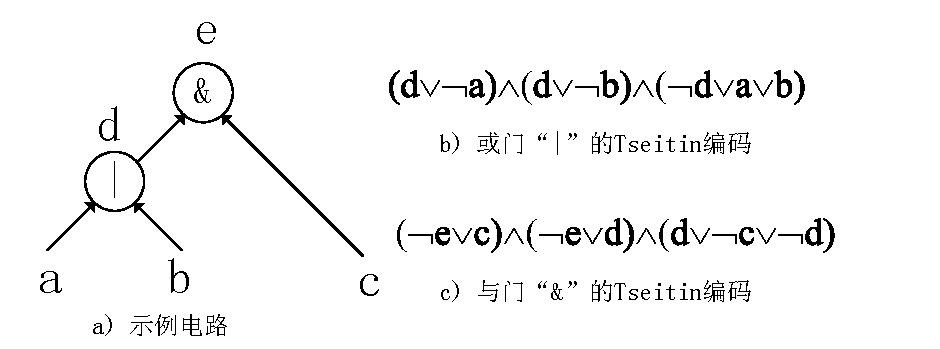
\includegraphics[width=0.8\textwidth]{fig_basic_circuit}
  \caption{示例电路及其编码}
  \label{basic_circuit}
\end{figure}


最简单的SAT求解算法是简单地遍历所有可能的变量赋值,形成树形的二叉搜索空间。对于图\ref{basic_circuit}b)的SAT公式,将导致图\ref{basic_search}所示的二叉搜索树。其中打钩的叶节点表示合法的求解结果。每次对特定变量进行二叉分解的步骤称为决策,每次决策产生一个新的决策层。图\ref{basic_search}的决策层1、2和3分别对应于分别对变量a、b和c进行二叉分解。

\begin{figure}[b] % use float package if you want it here
  \centering
  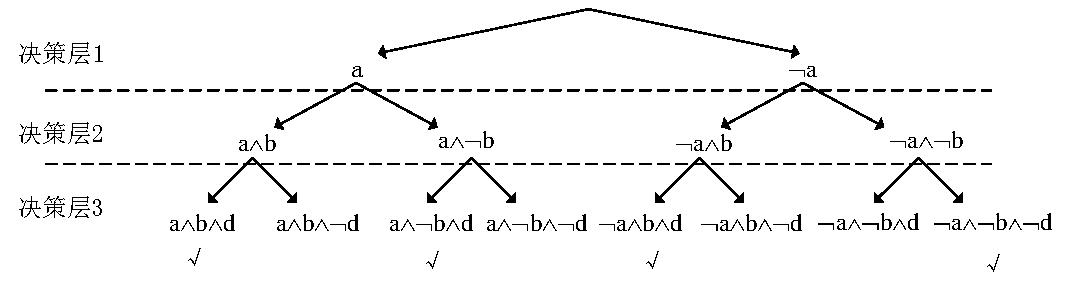
\includegraphics[width=0.8\textwidth]{fig_basic_search}
  \caption{基于完全二叉树遍历的SAT求解}
  \label{basic_search}
\end{figure}

\subsubsection{布尔约束传播(BCP)}
为了使一个特定的SAT公式成立,必须使其中每个子句都成立。
而为了使某个特定子句成立,其中必须存在至少一个文字成立。
因此当在某个子句中,只有一个特定的文字$w$尚未取值,而其他所有文字均取值为$0$时,
则该文字必须取值为$1$。
如果该文字为某个特定变量$v$,这将导致$v$取值为$1$,否则取值为$0$。
这一推导过程称为布尔约束传播。

以图\ref{basic_circuit}b)的或门的Tseitin编码为例,
为了使该公式成立,每个子句都必须成立。
以第一个子句$d \wedge a$为例,当$a$ 为$1$时,
$d \wedge a$化简为$d$,
为了使其成立,$d$必须取值为1。
此时搜索树如图\ref{BCP} 所示。
其中粗线代表在特定决策层内部的BCP 操作。

\begin{figure}[t] % use float package if you want it here
  \centering
  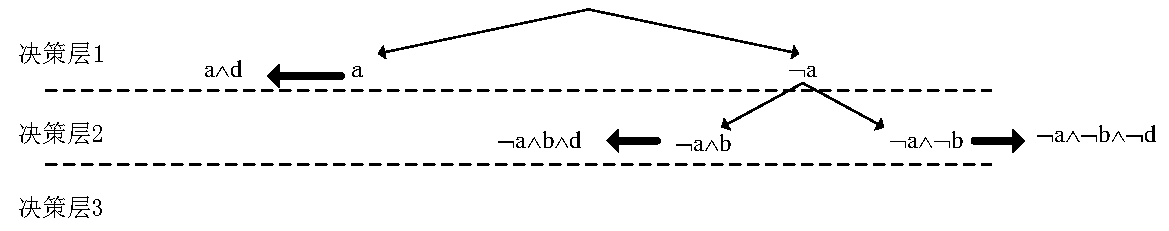
\includegraphics[width=0.8\textwidth]{布尔约束传播}
  \caption{布尔约束传播}
  \label{BCP}
\end{figure}

\subsubsection{冲突指导的子句学习}
冲突指导的子句学习和非正交回溯\upcite{DBLP:conf/iccad/ZhangM02} 是提升SAT求解器性能的另一个重要手段。其中非正交回溯与与本文重点关注的数据结构关系不大,因此将仅描述冲突指导的子句学习。

为了简明起见,仍然使用一个例子描述冲突指导的子句学习。如图\ref{confict}所示的一个二叉搜索树,当到达红色的标记为conflict 的节点时,有$\{a \equiv 0,b \equiv 0, c \equiv 0,d \equiv1,e \equiv 0,f \equiv1\}$。这将导致某个短句中的所有文字均成为0,称这种情况为一个冲突(conflict)。 此时冲突分析算法将对该子句中的每一个文字,沿着如图\ref{confict}粗线所示的BCP 关系逆向回溯,以便找到导致此次冲突的根本原因。假设找到的三个变量分别为$\{c \equiv 0,d \equiv 1,f \equiv 1\}$,这意味着a、b和e与本次冲突无关。无论以后a、b 和e 取任何值,只要遇到$\{c \equiv 0,d \equiv 1,f \equiv 1\}$ 的情况,都不必继续搜索。这意味图\ref{confict}中绿色所示的分支都可以被剪掉。

为了达到这种剪枝效果,将对冲突分析的结果中每个变量取反,以构造一个冲突学习子句。即$\{c \equiv 0, d \equiv 1, f \equiv 1\}$ 将会产生一个冲突学习子句$\{c\vee \neg d \vee \neg f\}$,并加入子句数组。以后每次当c、d和f三个变量中的两个满足$\{c \equiv 0, d \equiv 1, f \equiv 1\}$,则将立即通过冲突学习子句产生一次BCP,使得第三个变量无法满足$\{c \equiv 0,d \equiv 1,f \equiv 1\}$。 这就构成了一次剪枝操作。

\begin{figure}[t] % use float package if you want it here
  \centering
  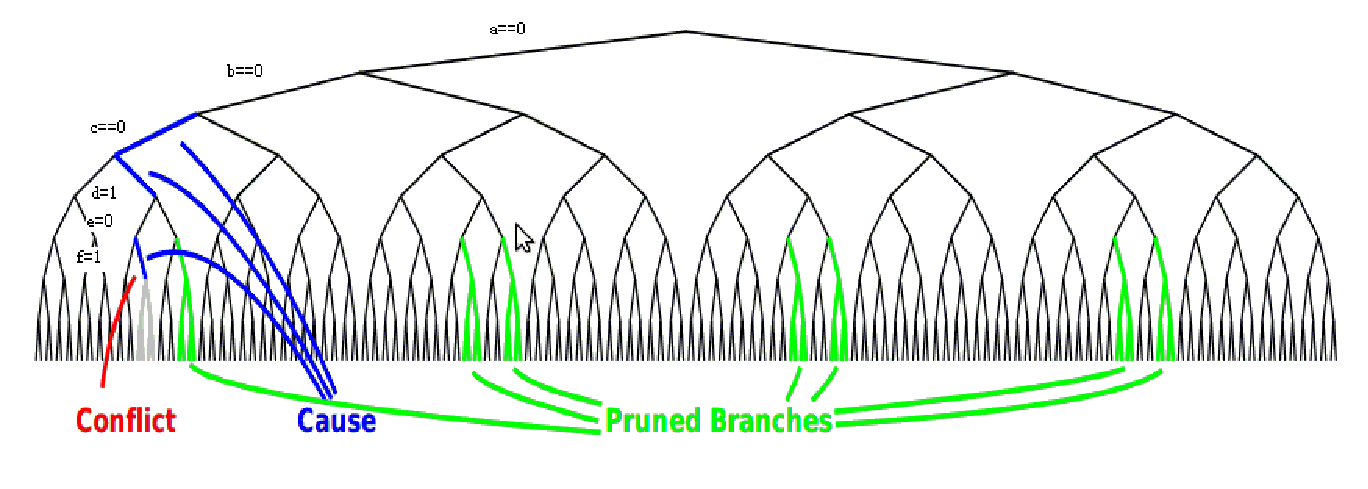
\includegraphics[width=0.8\textwidth]{fig_conflict}
  \caption{冲突指导的子句学习}
  \label{confict}
\end{figure}


\subsubsection{MiniSat 求解器的递增求解机制}\label{subsec_incsat}

本文中,
我们使用MiniSat 求解器\upcite{EXTSAT} 求解所有CNF公式。
和其他基于冲突学习机制\upcite{CONFLICTLEARN}的SAT求解器类似,
MiniSat 从在搜索中遇到的冲突中产生学习短句,
并记录他们以避免类似的冲突再次出现。
该机制能够极大的提升SAT求解器的性能。

在许多应用中,
经常存在一系列紧密关联的CNF公式。
如果在一个CNF公式求解过程中得到的学习短句能够被其他CNF公式共享,
则所有CNF公式的求解速度都能够得到极大的提升。

MiniSat 提供了一个增量求解机制以共享这些学习短句。
该机制包括两个接口函数:
\begin{enumerate}
\item
$addClause(F)$ 用于将一个CNF公式$F$ 添加到MiniSat的短句数据库,
以用于下一轮求解。
\item
$solve(A)$ 接收一个文字集合$A$作为假设,
并求解CNF 公式$F\wedge \bigwedge_{a\in A} a$。
其中$F$是在$addClause$中被加入短句数据库的CNF公式。
\end{enumerate}

基于该机制,
可以针对一个相同的CNF公式$F$,
使用不同的文字集合$A$,
来产生并递增地高效求解不同的$F\wedge \bigwedge_{a\in A} a$。


\subsection{可满足赋值遍历}\label{subsec_relallsat}
多数时候,可以满足特定SAT问题的解并不是唯一的,
求出所有可满足解的过程被称为可满足赋值遍历(简称ALLSAT求解)。

ALLSAT求解由基于SAT求解的可满足赋值遍历算法来实现。
直观上看,调用一次SAT求解器可以获得SAT问题的一个解,也就是一个完整的可满足赋值。
将这个完整的可满足赋值中每一个文字取反,构造出阻断(block)子句并加入到待求解的SAT问题公式中,
以引导SAT求解器避开已搜索过的解。
通过多次重复,最终可以获得SAT问题所有的解。

绝大多数可满足赋值遍历算法致力于将由SAT求解得到的一个完整的赋值扩展为一个包含较多赋值的赋值集合,
以便减少调用SAT求解器的次数并压缩存储赋值解的空间开销。
文献\upcite{SATUNBMC}提出了第一个此类算法。
他在SAT求解器求解过程中构造一个蕴含图,
用以记录每个赋值之间的依赖关系。
每个不在该图中的赋值变量都可以从最终结果中剔除。
在文献\upcite{MINASS} 和\upcite{REPARAM}中,
每个变量如果在其不被约束的情况下不能使$obj\equiv 0$ 被满足的话,
则该变量可以从最终结果中剔除。
在文献\upcite{MINCEX} 和\upcite{PRIMECLAUSE,EFFCON}中,
冲突分析方法被用于剔除与可满足性无关的变量。
在文献\upcite{MEMEFFALLSAT}中,
变量集合被划分为重要变量和非重要变量集合。
搜索过程中重要变量的优先级高于非重要变量。
因此重要变量子集构成了一个搜索树,
而该树的每一个叶节点是非重要变量的一个搜索子树。
%Tobias Nopper et al.\upcite{CMPMINCEX} propose an counterexample minimization algorithm for incomplete designs that contain black box.
Cofactoring \upcite{EFFSATUSMCCO} 则通过将非重要变量设置为SAT求解器返回的值以缩减搜索空间。

另一类算法通过Craig插值以扩大解集合。
文献\upcite{InterpBoolFunction}提出了第一个此类算法。
该算法构造两个相互矛盾的公式,并从他们的不可满足证明中抽取Craig 插值。
在文献\upcite{interpNoProof}中,
Craig插值的产生过程类似于传统的可满足赋值遍历算法。
不过其扩展算法包含两步,
分别对应于两个参与计算的公式。
该算法是第一个不需要产生不可满足证明的Craig插值算法。

\subsection{Craig插值的原理和实现}\label{sec_craigimp}
在通常的SAT求解器,
包括本文使用的MiniSat\upcite{EXTSAT}中,
要求待求解的公式被表示为CNF格式。
其中一个公式是多个子句的合取(conjunction),
而每一个子句是多个文字的析取(disjunction),
而每个文字是一个布尔变量$v$或者其反$\neg v$。
如公式$(v_0\vee\neg v_1\vee v_2)\wedge(v_1\vee v_2)\wedge(\neg v_0\vee v_2)$,
包含子句$v_0\vee\neg v_1\vee v_2$,$v_1\vee v_2$和$\neg v_0\vee v_2$。
而子句$v_0\vee\neg v_1\vee v_2$包含文字$v_0$, $\neg v_1$和$v_2$。

当存在一个变量$v$,
使得一个子句$c$中同时包含两个文字$v$和$\neg v$,
则称$c$为tautological的。
我们通常假设有待SAT求解器求解的公式中所有的子句都是非tautological的。

假设公式$F$的布尔变量全集为$V$。
若存在对$V$的赋值函数$A:V\to \{0,1\}$,
使得$F$中的每个子句均能取值为1,
则称$F$是可满足的,
此时SAT求解器能够找到赋值函数$A$。
否则称$F$为不可满足的,
此时SAT求解器能够产生如下一小节所述的不可满足证明。

\subsubsection{不可满足证明}
对于两个子句$c_1=v\vee A$和$c_2=\neg v\vee B$,
当$A\vee B$是tautological时,
$A\vee B$称为它们的\textbf{resolvant}。
而$v$称为它们的\textbf{pivot}。
易知以下事实:

\begin{equation}
\begin{array}{ccc}
&resolvant(c_1,c_2) = \exists v, c_1\wedge c_2 &\\
&c_1\wedge c_2 \to resolvant(c_1,c_2)&
\end{array}
\end{equation}

\begin{definition}
对于不可满足公式$F$,
假设其子句集合为$C$,
则其不可满足证明$\Pi$是一个有向无环图$(V_{\Pi},E_{\Pi})$,
其中$V_{\Pi}$是子句集合,
而$E_{\Pi}$是连接$V_{\Pi}$中子句的有向边集合。
$\Pi$满足如下要求:
\begin{enumerate}
\item 对于节点$c\in V_{\Pi}$:
  \begin{enumerate}
    \item 要么$c\in C$,此时称$c$为$\Pi$的根
    \item 或者$c$有且仅有两个扇入边$c_1\to c$和$c_2\to c$,
    使得$c$是$c_1$和$c_2$的resolvant。
  \end{enumerate}
\item 空子句是$\Pi$的唯一一个叶节点。
\end{enumerate}
\end{definition}

直观的说,
$\Pi$就是一棵树,
以子句集合$C$的子集为根,
以空子句为唯一叶节点。
而每个节点$c$的两个扇入边$c_1\to c$和$c_2\to c$代表了一个resolving关系$c:=resolvant(c_1,c_2)$。

包括本文使用的MiniSat求解器\upcite{EXTSAT}在内的许多SAT求解器,
当公式不可满足时都将产生一个不可满足证明$\Pi$。

\subsubsection{Craig插值算法}

根据文献\upcite{Craig},
给定两个布尔逻辑公式$A$ 和$B$,
若$A\wedge B$ 不可满足,
则存在仅使用了$A$ 和$B$共同变量的公式$I$ ,
使得$A\Rightarrow I$且
$I\wedge B$不可满足。
$I$ 被称为$A$针对$B$的Craig插值\upcite{Craig}。

目前最常见且最高效的产生Craig插值的算法是
McMillan算法\upcite{interp_McMillan} 。
其基本原理描述如下。

对于上述公式$A$和$B$,
已知$A\wedge B$不可满足,
而$\Pi$是SAT求解器给出的不可满足证明。
当一个变量$v$同时出现在$A$和$B$中时,
我们称其为全局变量。
若$v$只出现在$A$中,
则称其为$A$本地变量。

对于文字$v$或者$\neg v$,
当变量$v$是全局变量或者$A$本地变量时,
称该文字为全局文字或者$A$本地文字。

对于子句$c$,
令$g(c)$为$c$中所有全局文字的析取,
而$l(c)$为$c$中所有$A$本地文字的析取。

例如,
假设有两个子句$c_1=(a\vee b\vee\neg c)$ 和
$c_2=(b\vee c\vee\neg d)$。
并假设$A=\{c_1\}$和$B=\{c_2\}$。
则$g(c_1)=(b\vee\neg c)$,
$l(c_1)=(a)$,
$g(c_2)=(b\vee c)$,
$l(c_2)=FALSE$。


\begin{definition}\label{def_gencraig}
令$(A,B)$为一对公式,
而$\Pi$是$A\wedge B$的不可满足证明,
且其唯一叶节点是空子句$FALSE$。
对于每一个节点$c\in V_{\Pi}$,
令$p(c)$为如下定义的一个公式:
\begin{enumerate}
\item 如果$c$是根节点则
  \begin{enumerate}
    \item 如果$c\in A$则$p(c)=g(c)$
    \item 否则$p(c)=TRUE$
  \end{enumerate}
\item 否则令$c_1$和$c_2$分别是$c$的两个扇入节点,而$v$是他们的pivot变量
  \begin{enumerate}
    \item 如果$v$是$A$本地变量,则$p(c)=p(c_1)\vee p(c_2)$。
    \item 否则$p(c)=p(c_1)\wedge p(c_2)$。
  \end{enumerate}
\end{enumerate}
\end{definition}

上述定义\ref{def_gencraig}是构造性的,
已经给出了从不可满足证明$\Pi$得到最终的Craig插值的算法,
即以$\Pi$的根节点为起点,
为每一个$c$计算相应的$p(c)$,
直至到达最终的唯一叶节点$FALSE$。
我们有以下定理:

\begin{theorem}
定义\ref{def_gencraig}为唯一叶节点$FALSE$产生的$p(FALSE)$即为
$A$相对于$B$的Craig插值。
\end{theorem}

该定理的详细证明可见文献\upcite{DBLP:journals/tcs/McMillan05}。

计算$A$相对于$B$的Craig插值的时间复杂性为$O(N+L)$,
其中$N$是$\Pi$中包含的节点个数$|V_{\Pi}|$,
而$L$是$\Pi$中的文字个数$\Sigma _{c\in V_{\Pi}}|c|$。
而所产生的插值可以视为一个电路,
其空间复杂性为$|O(N+L)|$。
当然,
$\Pi$的尺寸在最坏情况下也是$A\wedge B$的尺寸的指数。

%\subsection{对偶综合}\label{subsec_relallsat}


\section{面向软硬件设计验证的可满足问题求解}
可满足问题(SAT)\upcite{SATtheory}是硬件电路设计和软件可信验证领域\upcite{HardwareSAT,softwareSAT} 共同关注的重要问题。许多重要的电路设计和软件验证问题均可转换为可满足性问题,并由SAT求解器求解。随着集成电路制造工艺的发展,在单个芯片内集成的晶体管个数将在2020年接近一千亿;而社会信息化程度的提高促使软件系统越来越复杂,以Linux操作系统为例,在2008 年仅其内核代码就已经突破1千万行。软硬件系统的规模日益增大,服务于硬件设计和软件验证的SAT求解器的运算量也急剧攀升。在过去的10年,作为形式化工具基本引擎的SAT 求解器性能已经显著提升,几分钟内即可处理数百万变量和数亿子句,但是依然无法满足日益增长的计算要求。

传统的硬件辅助与设计(EDA)综合与验证工具的核心框架通常包含以下主要功能模块:

1.抽象问题表示:该模块用于管理与特定推理过程和引擎无关,但是与问题本身密切相关的数据结构,如简化布尔电路(Reduced Boolean circuits)\upcite{DBLP:conf/tacas/AbdullaBE00}和
与非图(And-Inverter Graph)\upcite{Brummayer06localtwo-level}等。

2.问题编码:该模块用于将特定的抽象问题表示,转换为满足特定推理引擎,
如二叉决策图(简称BDD)\upcite{DBLP:journals/tc/Bryant86} 或SAT要求的数据结构,以便进行高效的推理工作。针对SAT推理引擎,该模块通常使用在空间和时间方面均具有多项式复杂性的Tseitin\upcite{Tseitin} 编码。

3.BDD和SAT推理引擎:这两个模块负责具体的推理工作。
绝大多数EDA工具和软件验证工具的核心推理引擎为二叉决策图(BDD)和可满足求解器(SAT)。其中BDD受到归一化表示方式导致的状态空间爆炸问题的困扰,通常仅用于需要归一化特性的小规模推理问题,如抽象谓词的表示等。而SAT则通常较少受到状态空间爆炸的影响,且天生具有内在的并行性和可扩展性;另一方面SAT问题是NP难问题,其求解时间和问题结构相关,对计算资源的需求也随具体问题而不同。

软件程序验证工具也具有类似于硬件设计验证工具的核心框架。
SAT求解器通常是作为核心推理引擎集成到具体问题求解器中。
因此,从逻辑流程上看,
硬件和软件形式化验证通常都是通过抽象问题表示之后再进行问题编码,
而后将问题的可满足性求解过程交给SAT 求解器完成,
流程如图\ref{verfication-procedure}所示。

\begin{figure}[t] % use float package if you want it here
  \centering
  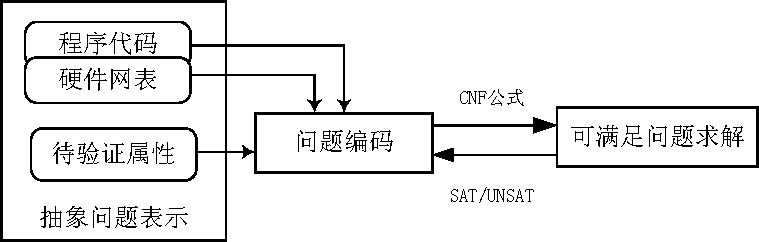
\includegraphics[width=0.8\textwidth]{验证流程}
  \caption{基于SAT求解的软硬件验证流程}
  \label{verfication-procedure}
\end{figure}

因此将软硬件设计验证中产生的复杂SAT 问题外包到云或网格环境下,利用其提供的弹性计算资源,成为一种有吸引的解决方案。
科研机构和商业公司也已经开展了在云和网格环境下进行SAT问题求解的研究
\upcite{DBLP:conf/IEEEcloud/BrunM12,Nordugrid,DBLP:journals/concurrency/ChrabakhW07,OneSpin,CloudSMT}。
如美国华盛顿大学研究小组推出支持云SAT求解的sTile系统\upcite{DBLP:conf/IEEEcloud/BrunM12};
芬兰阿尔托大学研究小组推出基于NorduGrid的SAT求解器\upcite{Nordugrid};
美国圣巴巴拉大学研究小组推出GridSAT系统\upcite{DBLP:journals/concurrency/ChrabakhW07};
形式化验证服务提供商OneSpin 公司和Plunify公司于2013年,
联合推出了面向云平台的基于SAT求解的硬件验证商业服务\upcite{OneSpin}。

\section{开放环境下数据隐私的安全威胁}
云计算和网格依托于互联网,与互联网这种开放环境的便利快捷相伴而生的是,安全威胁也无处不在。
一方面,公有云和网格计算节点均直接部署在广域网上,与用户处于不同的安全域。
用户的服务请求可能面临来自网络中的多重威胁;
另一方面,云服务提供商或是网格计算节点无法证明其内部行为可以信任。

由于网格计算是由松散耦合的高端计算设施组成\upcite{Nordugrid},网格环境下恶意计算节点是客观存在的\upcite{HV-grid};
而在云计算环境下,虽然云硬件平台提供商及其基础设施(虚拟层)是可被信赖,在其上运行的虚拟机却不总是可以信赖的。
文献\upcite{AMI}指出,著名的云计算提供商亚马逊的EC2受到了虚拟机影像滥用的困扰,被污染虚拟机映像会迅速扩散到整个社区;
而文献\upcite{InformationLeakageofCloud} 则指出了处于同一台物理机器上的虚拟机之间攻击的可能性。
与此相照应,早在2007年,
《华盛顿邮报》就披露了客户关系管理领域著名的云服务提供商Saleforce.com由于受到安全攻击而导致大量租户数据泄露与丢失\upcite{washingtonPostSaleForce};
2010 年下半年谷歌解雇了两名入侵租户的私有账户以获取隐私数据的员工\upcite{googelFiresTwoEmployees}。
Gartner 公司发布的研究报告\upcite{gartner70}显示,所采访的企业中70\%以上认为出于对数据安全性与隐私保护的怀疑,
在近期内不会采用云计算技术。
RSA 首席技术官也指出\upcite{rsaSafe},在企业将现有的应用向第三方云服务提供商提供的云环境迁移过程中,
要考虑的首要问题是对云计算的数据安全问题。
此处的安全不仅指数据的可用,更加注重的是数据的隐私保护。
针对OneSpin公司推出的硬件形式化验证云服务,新闻评论\upcite{oneSpinsafe}指出验证数据的隐私是用户最为关心的因素。

而针对计算结果的安全性,对早期的志愿计算SETI@home项目的统计发现\upcite{HV-grid},这类基于网格的开放计算环境存在三类威胁:
\textbf{私心的计算参与者}:由于计算结果具有稀缺性,私心的计算参与者会出现奇货可居的意识,他们会完全遵照协议的规定,尽力计算出正确结果,但会出于利益原因,将有价值的结果信息透露给第三方,从而损害用户的隐私安全。
\textbf{懒惰的计算参与者}:由于大计算量会耗费很多计算资源,出于节约计算成本的考虑,计算参与者可能不按照约定来进行足量的计算,以此来节省开销,使用部分结果来作为最终结果。
\textbf{恶意的计算参与者}:可能出于某种目的,计算参与者完全违反协议规定,随意返回错误结果来欺骗用户,误导用户决策。
而在2009年对云计算模型和网格计算模型的比较一文\upcite{DBLP:journals/corr/abs-0901-0131} 中,Ian Foster 指出云计算在安全措施设计成熟度还远不及网格,这就使得网格计算下影响结果正确性的威胁也很可能对云计算环境造成影响。

这些事实指出,外包到云计算或网格这类开放环境下的SAT问题,
由于计算模式将数据和处理的控制权从用户转移至云服务方,导致具体的处理过程用户不可控;
其输入和输出数据可能会被未授权的第三方访问,
这些潜在的威胁者可能会从这些数据中获取有价值的信息。
糟糕的是,即使发生了上述信息泄露的情况,如果不辅助以技术手段,用户难以察觉和追踪;
更为恶劣的情况是,部署在网格或云环境下的SAT求解器可能会被迫使返回错误的结果。

来源于软硬件验证的SAT问题,可能遭受硬件结构信息泄露的问题;Roy\upcite{csRoy} 和Fu\upcite{csFu}的工作指出了从CNF 公式中抽取电路结构信息的可能性。Zvika\upcite{OBfuscationd-CNFs}、Yuriy Brun\upcite{DBLP:conf/IEEEcloud/BrunM12} 等人的工作也指出在云计算环境下进行SAT问题求解需要解决隐私保护问题。另一方面,Du\upcite{HV-grid} 将某些复杂SAT问题的解称作高价值稀有事件,指出SAT问题的解也应该被视作为隐私;如来源于密码破解的SAT问题,奇货可居的计算参与者可能会因利益问题而将其泄露给第三方。

\section{开放计算环境下可满足问题求解的隐私保护问题}
开放环境下的这些威胁将SAT计算服务的潜在用户置于进退维谷的境地:
使用公共的云计算或网格计算基础设施在系统维护性和可用性上面具有较高的性价比,
但却会面临隐私泄露和错误结果等安全问题的困扰。
在开放计算环境下,计算数据的隐私保护问题看起来是一个不可能完成的问题:由于计算是在开放环境下完成的,未经加密处理的原始输入和输出数据势必会引发泄露的风险,而经过传统加密算法处理之后的计算数据由于对计算不再透明,因而丧失了可计算性。因此在保持可计算性的前提下,讨论SAT数据的隐私保护,成为了开放计算环境下的最大挑战。

2009 年,Gentry 等人针对开放计算环境下的数据隐私保护问题,提出完全同态加密的概念。
这一概念描绘了开放环境下计算外包的美好愿景:经过完全同态加密,在保持数据隐私性的同时,仍然可保持原有数据的可计算性。完全同态加密的理论基础是,由于任何计算都可以分解为一系列微观加乘计算,并且在有限步内对加乘计算透明的加密算法确实存在。
因而任意的计算都可以分解为一系列的有限次针对加密数据的加乘计算。
这无疑从理论上扫清了开放环境下计算外包的安全障碍。但是,由于完全同态加密需要将计算分解为细粒度的有限步加乘计算。
所带来的昂贵计算开销,使其距离实用化还有相当的距离。

同样为了解决外包计算的数据隐私保护,Atallah等提出了针对具体问题,进行计算数据伪装的概念。例如针对矩阵求解类计算,将有待外包的数据与随机对角矩阵进行矩阵乘,对外包的矩阵数据进行伪装加密。
由于矩阵计算的可逆性,伪装加密后结果可以通过可逆的矩阵运算得到。数据伪装方法充分利用了问题的特点,不改变原有计算过程和数据的外在形式,是一种直接实用的方案。但目前针对SAT 问题的数据伪装的研究还处于空白。

作为一种基础的计算引擎,软硬件设计问题中的SAT问题具有其内在的特点:任何硬件设计和软件程序都可以表示为与或非等门的集合。
本文从实用化的角度出发,希望在复用原有求解器的前提下,探讨软硬件设计、验证领域中SAT 问题的隐私保护方法。

\subsection{CNF公式中的结构信息}\label{CNF structure}
%\textbf{Circuit structure in CNF formula}\label{CNF structure}
%Since we want to protect circuit structure in CNF formula,
%let's first study how the circuit can be recovered from CNF formula.
%Literatures\upcite{csRoy,csFu} have proposed algorithms to recover circuit structure from CNF formula in details.
%Before discussing them, some concepts should be introduced first.
CNF公式是SAT求解的输入数据,来源于软硬件验证及设计中的CNF公式中会包含硬件电路结构信息;
文献\upcite{csRoy,csFu}给出了从CNF公式中获取电路结构信息的算法细节,首先了解算法中用到的概念。
%
%\begin{definition}[CNF signature]
%CNF signature of gate $g$ is its Tseitin encoding $Tseitin(g)$.
%Each clause in CNF signature is called characteristic clause.
%A characteristic clause containing all variables in CNF signature is a \textbf{key clause}.
%Variable corresponding to output of a gate is called \textbf{output variable}.
%\end{definition}
\begin{definition}[CNF标记]
门$g$的CNF标记就是它的Tseitin编码$Tseitin(g)$。
CNF标记中的每个子句称为门的\textbf{特征子句}。
包含门中所有变量的特征子句称为\textbf{关键子句}。
对应于门输出的变量称为\textbf{输出变量}。
\end{definition}

公式(\ref{eqn_andinv})中的 AND2门,
$\neg e\vee c$ 是它的一个特征子句,
$e\vee \neg c\vee\neg d$是它的关键子句。
$e$是输出变量。

文献\upcite{csRoy}指出,
在一种编码规则下,具有相同特征函数的门必然会被编码成为相同的CNF 标记,也就是相同的子句集合。
通过探索这种结构特征可以恢复电路结构,已知的结构检测算法基于以下定义的有向超图和二分图概念。

\begin{definition}[超图]\label{Hypergraph}
 以CNF公式中的子句为节点、变量为边,形成的图称为超图(Hypergraph)。
 超图$G(V,E)$ 中:
 $V$中每个节点对应$F$中一个子句;
 $E$中每条边对应$F$中一个变量。
 如果两个子句包含相同的变量,就在两个子句之间连接一条边,并用变量标注。
\end{definition}

在超图表示方式下,存在具有不同CNF标记的两个门,却具有相同超图表示的情况,
如AND3和OR3,均对应图\ref{graph}a)中的超图。
为了克服该问题,在电路结构检测算法\upcite{csRoy}中,使用有向超图进行区分。

\begin{definition}[有向超图]
在定义\ref{Hypergraph}给出的超图基础上,
根据子句中文字的正负、为边添加标记,
形成的图称为有向超图(Directed Hypergraph)。
\end{definition}

\begin{definition}[二分图]
将子句和变量均视为节点,同时将变量和子句的从属关系视为边,形成的图称为二分图(Bipartite Graph)。
在二分图$G(V,E)$中:
$V$中每个顶点对应于集合中的一个子句或一个变量,即$V=V_{cls}\bigcap V_{var}$,其中$V_{cls}$为子句集合、$V_{var}$ 为变量集合。
$E$中的每条边对应于一个子句/变量对,
如果变量出现在子句中,就在变量和子句之间连接一条边;变量为负值则对应一条负边,反之为正边。
\end{definition}

以AND门为例,AND3门的超图如图\ref{graph}a)所示;
其有向超图对应于图\ref{graph}b),其中使用$\uparrow$表示正,┼ 表示负;
其二分图对应于图\ref{graph}c) 所示的二分图。
\begin{figure}[t]
  \centering
  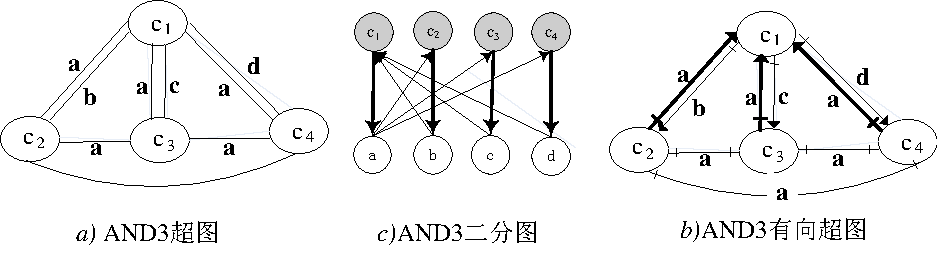
\includegraphics[width=0.8\textwidth]{超图二分图}
  \caption{超图和二分图}
  \label{graph}
\end{figure}

基于上述定义,CNF公式可以表示为包含多种CNF特征子图的超图或二分图。
这种图结构使得利用基于子图同构和模式匹配技术来恢复出电路结构和程序结构信息成为可能。

\subsection{SAT问题隐私保护的对象}
基于上述概念,
CNF公式可以转化超图$G$,
在图中匹配常用的CNF标记,通过同构子图的方式即可恢复出CNF公式携带的门信息。
进一步,可用最大无关集来表示恢复出来的电路信息。
基于关键子句和CNF标记的模式匹配还可以检测出所有门,并构建最大匹配门的子集。
除了门的结构信息,在来源于软硬件验证的CNF公式还包含了状态迁移关系。
Roy\upcite{csRoy}和Fu\upcite{csFu} 给出了具体的实现技术。
潜在的攻击者可以利用这些技术手段恢复出电路结构,并得到电路的状态迁移关系。
因此,CNF标记和关键子句是特别需要保护的重要信息。

另一方面,在验证领域,某些SAT问题的解反映了该系统的某些特性是否达到,因此解也应作为隐私加以保护。

\section{本文的主要工作}
来源于软硬件验证和设计的SAT 问题,
由于其CNF公式和其解中包含了电路结构以及电路迁移关系等敏感信息,在开放计算环境下求解,必须防止这些敏感信息的泄露。
本文的工作也围绕着保护上述敏感信息展开。

\subsection{已有工作的局限}
针对开放计算环境下的计算数据隐私保护问题,2009年Gentry\upcite{DBLP:conf/stoc/Gentry09} 等人开创性提出完全同态加密的概念。
经过完全同态加密,在保持数据隐私性的同时,仍然可保持原有数据的可计算性。由于任何的计算都可以分解为一系列微观加乘计算,因此寻找可保持对加乘的加密算法成为了一个努力的方向。
但是由于计算需要被分解为细粒度的有限步的加乘操作,因此同态加密后的计算效率一直制约着该方法的实用化。

针对CNF公式隐私保护方面相关的研究才刚刚开始,2013年Brakerski\upcite{OBfuscationd-CNFs} 等人面向云计算环境,首次探讨了使用多线性映射和坡度编码策略对d-CNF进行混淆的方法。
使用随机和带有噪声的编码,并提供测试过程来确保编码元素的等价。
这种方法基于有限加速假设,混淆后的CNF使用最原始的二叉树搜索的方法进行求解,无法利用目前经典的SAT求解器。

Yuriy Brun\upcite{DBLP:conf/IEEEcloud/BrunM12} 等人则使用了stile数据分布的模式,通过将数据条块计算,提高攻击者获得完整CNF 公式难度,以此降低数据被窃取的可能性。
该方法目前也仅仅支持简单的二叉遍历赋值求解方法,无法利用已有的SAT 求解加速算法。

上述的工作都试图重新构造求解器,无法利用目前已有的求解器研究成果。

\subsection{研究内容与创新点}
鉴于目前的研究现状,本文力图从SAT问题特性出发,寻求具有实用性的隐私保护方法。图\ref{fig:103}给出了本文的主要研究内容。

\begin{figure}[t] % use float package if you want it here
  \centering
  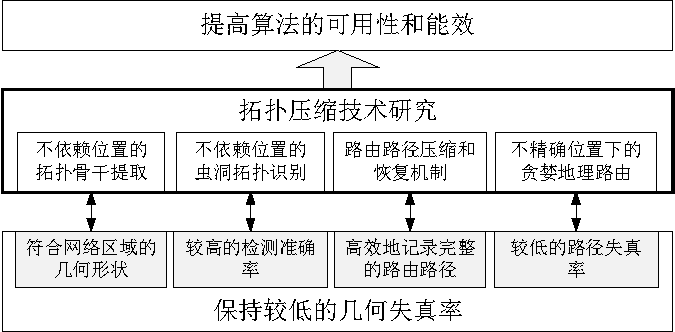
\includegraphics[width=0.8\textwidth]{fig103}
  \caption{本文研究内容}
  \label{fig:103}
\end{figure}

本文受国家高技术研究和发展计划“智能云服务与管理平台核心软件及系统”(项目编号2013AA01A212)和国家自然科学基金项目“面向通讯应用的自动对偶综合研究”(项目编号61070132)的支持,主要贡献和创新点如下:

1. 开放环境下基于加噪CNF混淆的SAT求解框架。
CNF公式混淆是保证开放环境下的SAT求解隐私性的重要手段。现有的方法基于双射或多射群加密,通过分段坡度编码对CNF 公式进行混淆,从而隐藏CNF公式中携带的结构信息。
但是这种方法改变了原有CNF公式的外部表示,需要设计新的求解算法。
并且在目前仅可使用全空间遍历的方法进行求解,无法利用已有成熟的SAT 求解算法,因此极大降低了其实用性。
本文通过对CNF公式自身逻辑特点的分析,提出了基于加噪思路的混淆算法。通过在原始CNF公式中无缝的混入噪音公式,在隐藏原有的结构信息的同时,保持原有的CNF 数据形式和解空间,从而复用目前已有的求解算法。
这就在算法的实用性和隐私保护上取得了良好的折中。
本文从理论上证明了算法的正确性并通过大量的仿真实验验证了算法的性能。

2. 解空间上估计的CNF混淆算法。
由于SAT求解时,输出数据也包含了敏感信息。
在研究了隐藏结构信息的CNF混淆算法之后,本文进一步研究了隐藏CNF 解的混淆方法。针对输出信息保护,本文提出了解空间上估计的CNF混淆算法。
通过扩展噪音公式解空间,使得混淆后SAT问题的解空间为原始解空间的上估计。
通过引入噪音解实现对原始解的隐藏。
本文从理论上充分证明了算法的正确性,并通过大量的仿真实验验证了方法的有效性和性能。

3. 混淆后公式的求解效率是在混淆算法有效性的一个特别重要的指标,也是基于加噪的混淆算法区别于其他混淆算法的一个重要因素。
由于加噪的过程改变了公式的内在结构,并且SAT问题自身特点,使得其问题复杂度会随着结构的变化出现跃变。
针对这一情况,本文针对硬件验证中常用的CNF结构进行分析,提出了跃变敏感的混淆策略,使得混淆后的CNF公式求解难度不会大于原始公式求解难度。
特别针对对偶综合这一SAT问题的实例算法进行了分析。从理论上验证了算法的可用性。

4. CNF混淆算法的有效性评价。
混淆算法保证混淆后的CNF公式可用已有的求解器求解,并且可以用较小的开销恢复出原始的解。
但是除此之外,在开放环境下为保证SAT 计算外包的顺利实施,混淆算法仍然需要满足其他的特性。
结合程序混淆的有效性评价标准,本文抽象出CNF公式混淆的有效性评价标准。
通过对混淆策略的细分,针对两种混淆策略进行定量分析和定性评价,为设计出更好的混淆策略提供了依据。

上述各部分研究内容之间的关系参见图1.3。
\section{论文组织结构}
论文共分六章,组织结构如下:
%TO DO 论文共分七章,组织结构如下:

第一章为绪论,介绍SAT求解的基本概念、特点、应用以及安全可验证计算的研究现状。分析CNF公式混淆算法的研究意义和挑战,并简述本文的研究内容和组织结构;

第二章为相关研究,对科学计算外包隐私保护、安全可验证计算以及程序混淆等相关概念进行了系统和全面的介绍,分析了现有工作的特点和适用性;

第三章研究SAT问题求解中输入数据的隐私保护问题,从实用性的角度出发,提出了基于加噪的CNF混淆算法。
在保证求解算法和解空间不变的前提下,通过混入噪音变量和子句来实现CNF公式内部结构信息的隐藏;

第四章在前述开创性工作的基础上,针对高危险外包计算环境,针对可能出现的ALLSAT攻击,通过引入具有簇形解的噪声CNF 公式,进一步提高混淆算法的鲁棒性;

第五章研究SAT问题求解中输出数据的隐私保护问题,提出了解空间上估计的CNF混淆方法,通过混入用户可剔除的噪声解来隐藏真实的解信息;
另一方面,研究SAT问题求解中输入数据中结构信息的增强型隐藏方法,提出在感知原有公式结构的基础之上,加入可构成合法结构的噪声变量和子句,来实现CNF公式内部结构的保真隐藏,以提高应对基于模式识别和同构检测等隐私攻击的防范能力;

%%第六章研究相变敏感的混淆算法,希望对混淆后的CNF公式求解效率进行有效控制。
第六章研究SAT问题混淆算法的有效性评价问题,希望通过对有效性标准的提取,为设计更为有效的混淆算法提供指导。
%
%第七章总结全文并展望未来的工作。

第七章总结全文并展望未来的工作。
最后是致谢、博士期间撰写的论文、参加的科研工作以及参考文献。

% !Mode:: "Tex:UTF-8"
\chapter{基于余因子和Craig插值的迭代特征化算法}
\label{chap:2}



\section{问题描述}

在形式化验证和综合领域,
对于两个存在某种内在联系的逻辑向量$\vec{a}$和$\vec{b}$,
有两种不同的方式表达他们之间的联系:关系和函数。

其中,
关系$R(\vec{a},\vec{b})$更具一般性,
能够表达$\vec{a}$和$\vec{b}$之间的任意对应。
尤其是一对多的对应,
这是关系比函数具有更强描述能力的地方。
这种一般性在形式化验证中广泛用于描述非确定性行为以扩展描述能力,
以及构造抽象模型\upcite{DBLP:conf/cav/ClarkeGJLV00}以削减计算复杂性等。

而另一方面,
函数是关系的一种受限形式。
如果$R(\vec{a},\vec{b})$满足以下要求,
则能将其转换为相应的函数$\vec{b}:=f(\vec{a})$:
对$\vec{a}$的任意取值$x\in[\![\vec{a}]\!]$,
均存在且仅存在唯一的$y\in[\![\vec{b}]\!]$,
使得$R(\vec{a},\vec{b})$。
在实际的软硬件设计与验证领域,
存在大量的情况需要从一个关系中获得相应的函数。
如在自动激励生成算法中从约束描述产生相应的激励函数\upcite{DBLP:conf/dac/YuanAAP03},
证明导引抽象中的抽象模型构造\upcite{DBLP:conf/fmcad/AmlaM04},
以及本文中推导控制流谓词和特征化解码器等。

以图\ref{fig_relation}为例。
对于图\ref{fig_relation}a)中的一对一映射,
我们可以使用布尔函数$y_1=x_1\wedge x_2$和$y_2=\neg x_1\wedge \neg x_2$表示。
而另一方面,
对于图\ref{fig_relation}b)中的布尔关系,
并不存在相应的布尔函数,
因为$(x_1,x_2)=(0,1)$的情形被映射到了多个$(y_1,y_2)$的组合。
而这种情况可以使用布尔关系$R=(\neg x_1\wedge\neg x_2\wedge \neg y_1\wedge y_2)
\vee(\neg x_1\wedge x_2\wedge \neg y_1\wedge \neg y_2)
\vee(\neg x_1\wedge x_2\wedge y_1\wedge y_2)
\vee(x_1\wedge \neg x_2\wedge \neg y_1 \wedge \neg y_2)
\vee(x_1\wedge x_2\wedge y_1\wedge \neg y_2)$。

\begin{figure}[t]
\begin{center}
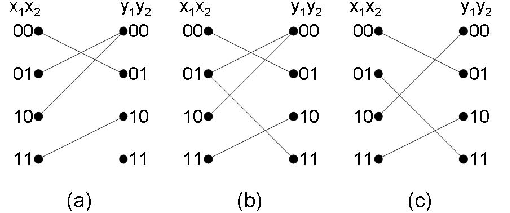
\includegraphics[width=\textwidth]{relation}
\end{center}
\caption{关系和函数的布尔映射}
  \label{fig_relation}
\end{figure}



在本章中,
我们首先在小节\ref{sec_craigimp}描述Craig插值的基本原理,
然后在小节\ref{sec_iterativecraig}中将其扩展到包含额外变量$\vec{c}$ 的更一般情形$R(\vec{a},\vec{b},\vec{c})$。

\section{Craig插值的原理和实现}\label{sec_craigimp}
注意本小节描述的Craig插值基本原理不是我们的原创,
而是为了方便上下文的叙述从\upcite{DBLP:conf/cav/McMillan03} 移植至此。
\subsection{相关背景知识和记法}
在通常的SAT求解器,
包括本文使用的MiniSat\upcite{EXTSAT}中,
要求待求解的公式被表示为CNF格式。
其中一个公式是多个短句的合取(conjunction),
而每一个短句是多个文字的析取(disjunction),
而每个文字是一个布尔变量$v$或者其反$\neg v$。
如公式$(v_0\vee\neg v_1\vee v_2)\wedge(v_1\vee v_2)\wedge(\neg v_0\vee v_2)$,
包含短句$v_0\vee\neg v_1\vee v_2$,$v_1\vee v_2$和$\neg v_0\vee v_2$。
而短句$v_0\vee\neg v_1\vee v_2$包含文字$v_0$, $\neg v_1$和$v_2$。

当存在一个变量$v$,
使得一个短句$c$中同时包含两个文字$v$和$\neg v$,
则称$c$为tautological的。
我们通常假设有待SAT求解器求解的公式中所有的短句都是非tautological的。

当存在一个假设公式$F$的布尔变量全集为$V$。
若存在对$V$的赋值函数$A:V\to \{0,1\}$,
使得$F$中的每个短句均能取值为1,
则称$F$是可满足的,
且SAT求解器能够找到赋值函数$A$。
否则称$F$为不可满足的。

\subsection{不可满足证明}
对于两个短句$c_1=v\vee B$和$c_2=\neg v\vee C$,
当$A\vee B$是非tautological的时,
$A\vee B$称为他们的resolvant。
而$v$称为他们的pivot。
易知以下事实:

\begin{equation}
\begin{array}{ccc}
&resolvant(c_1,c_2) = \exists v, c_1\wedge c_2 &\\
&c_1\wedge c_2 \to resolvant(c_1,c_2)&
\end{array}
\end{equation}

\begin{definition}
对于不可满足公式$F$,
假设其短句集合为$C$,
则其不可满足证明$\Pi$是一个有向无环图$(V_{\Pi},E_{\Pi})$,
其中$V_{\Pi}$是短句集合,
满足如下要求:
\begin{enumerate}
\item 对于节点$c\in V_{\Pi}$:
  \begin{enumerate}
    \item 要么$c\in C$,此时称$c$为$\Pi$的根
    \item 或者$c$有且仅有两个predecessors $c_1$和$c_2$,
    使得$c$是$c_1$和$c_2$的resolvant。
  \end{enumerate}
\item 空短句是$\Pi$的唯一一个叶节点。
\end{enumerate}
\end{definition}

直观的说,
$\Pi$就是一棵树,
以短句集合$C$的子集为根,
以空短句为唯一叶节点。
而每个节点的两个扇入边代表了一个resolving关系。

包括本文使用的MiniSat求解器\upcite{EXTSAT}在内的许多SAT求解器,
当公式不可满足时都将产生一个不可满足证明$\Pi$。

\subsection{Craig插值算法}

根据文献\upcite{Craig},
给定两个布尔逻辑公式$A$ 和$B$,
若$A\wedge B$ 不可满足,
则存在仅使用了$A$ 和$B$共同变量的公式$I$ ,
使得$A\Rightarrow I$且
$I\wedge B$不可满足。
$I$ 被称为$A$针对$B$的Craig插值\upcite{Craig}。

目前最常见且最高效的产生Craig插值的算法是
McMillan算法\upcite{interp_McMillan} 。
其基本原理描述如下。

对于上述公式$A$和$B$,
已知$A\cup B$不可满足,
而$\Pi$是SAT求解器给出的不可满足证明。
当一个变量$v$同时出现在$A$和$B$中时,
我们称其为全局变量。
若$v$只出现在$A$中,
则称其为$A$本地变量。

对于文字$v$或者$\neg v$,
当变量$v$是全局变量或者$A$本地变量时,
称该文字为全局文字或者$A$本地文字。

对于短句$c$,
令$g(c)$为$c$中所有全局文字的析取,
而$l(c)$为$c$中所有$A$本地文字的析取。

例如,
假设有两个短句$c_1=(a\vee b\vee\neg c)$ 和
$c_2=(b\vee c\vee\neg d)$。
并假设$A=\{c_1\}$和$B=\{c_2\}$。
则$g(c_1)=(b\vee\neg c)$,
$l(c_1)=(a)$,
$g(c_2)=(b\vee c)$,
$l(c_2)=FALSE$。


\begin{definition}\label{def_gencraig}
令$(A,B)$为一对公式,
而$\Pi$是$A\cup B$的不可满足证明,
且其叶节点是$FALSE$。
对于每一个节点$c\in V_{\Pi}$,
令$p(c)$为如下定义的一个公式:
\begin{enumerate}
\item 如果$c$是根节点则
  \begin{enumerate}
    \item 如果$c\in A$则$p(c)=g(c)$
    \item 否则$p(c)=TRUE$
  \end{enumerate}
\item 否则令$c_1$和$c_2$分别是$c$的两个扇入节点,而$v$是他们的pivot变量
  \begin{enumerate}
    \item 如果$v$是$A$本地变量,则$p(c)=p(c_1)\vee p(c_2)$。
    \item 否则$p(c)=p(c_1)\wedge p(c_2)$。
  \end{enumerate}
\end{enumerate}
\end{definition}

上述定义\ref{def_gencraig}是构造性的,
已经给出了从$\Pi$得到最终的插值的算法,
即以$\Pi$的根节点为起点,
为每一个$c$计算相应的$p(c)$,
直至到达最终的唯一叶节点$FALSE$。
我们有以下定理:

\begin{theorem}
定义\ref{def_gencraig}为唯一叶节点$FALSE$产生的$p(FALSE)$即为
$A$相对于$B$的Craig插值。
\end{theorem}

该定理的详细证明可见文献\upcite{DBLP:journals/tcs/McMillan05}。

计算$A$相对于$B$的Craig插值的时间复杂性为$O(N+L)$,
其中$N$是$\Pi$中包含的节点个数$|V_{\Pi}|$,
而$L$是$\Pi$中的文字个数$\sigma_{c\in V_{\Pi}}|c|$。
而所产生的插值可以视为一个电路,
其空间复杂性为$|O(N+L)|$。
当然,
$\Pi$的尺寸在最坏情况下也是$A\cup B$的尺寸的指数。



\section{非迭代的特征化算法}

假设有布尔关系$R(t,\vec{a})$使得
$R(1,\vec{a})\wedge R(0,\vec{a})$不可满足。
而我们需要从$R$中特征化函数$f$,
使得$t=f(\vec{a})$。
则根据上述的讨论,
可以简单的令$A=R(1,\vec{a})$而$B=R(0,\vec{a})$。
此时$A$相对于$B$的Craig插值,
即为函数$f$的一个实现。

该算法在本文的后继章节中被广泛应用于构造解码器的布尔函数。


\section{迭代的特征化算法}\label{sec_iterativecraig}
上一小节讨论了如何从关系$R(a,\vec{b})$特征化函数$a=f(\vec{b})$。
然而在更一般的情形下,我们需要从$R(\vec{a},\vec{b},t)$特征化函数$t=f(\vec{a})$。
相比之下,此时多了一个需要进行存在性量化的$\vec{b}$。
为此我们需要将上述算法进行以下扩展。

假设$R(\vec{a},\vec{b},t)$是一个使得$R(\vec{a},\vec{b},0)\wedge R(\vec{a},\vec{b},1)$ 不可满足的布尔公式。

其中$\vec{a}$ 和$\vec{b}$ 被分别称为重要和非重要变量子集。
而$t$ 是目标变量。
我们进一步假设$R(\vec{a},\vec{b},t)$ 是可满足的。

我们需要特征化一个布尔函数$FSAT_R(\vec{a})$,
覆盖且仅覆盖了所有能够使得$R(\vec{a},\vec{b},1)$ 可满足的$\vec{a}$。
形式化的定义是:

\begin{equation}\label{fchar}
% \begin{split}
FSAT_R(\vec{a}):=
\left\{
\begin{array}{rcl}
1 & & \exists\vec{b}.R(\vec{a},\vec{b},1) \\
0 & & otherwise
\end{array}
\right.
% \end{split}
\end{equation}
%% HAHA come to here

因此,
一个计算$FSAT_R(\vec{a})$ 的简单算法是:
逐一遍历并收集所有使得$R(\vec{a},\vec{b},1)$ 可满足的$\vec{a}$的赋值。
然而该算法需要处理$2^{|\vec{a}|}$中情况。
对于很长的$\vec{a}$,时间开销将会很大。

使用cofactoring \upcite{EFFSATUSMCCO} 和Craig 插值\upcite{interp_McMillan},
可以将每一个$\vec{a}$ 扩展为一个更大的集合,
从而极大的提高算法运行速度。
直观的,
假设$R(\vec{a},\vec{b},1)$ 的一个满足赋值是$A:\vec{a}\cup\vec{b}\cup\{t\}\to\{0,1\}$,
通过cofactoring\upcite{EFFSATUSMCCO}可以构造以下公式:

\begin{algorithm}[t]
\caption{$CharacterizingFormulaSAT(R,\vec{a},\vec{b},t)$: 特征化使得$R(\vec{a},\vec{b},1)$ 可满足的$\vec{a}$ 集合}
\label{alg_craigchar}
%\KwIn{The Boolean formula $R(\vec{a},\vec{b},t)$,
%its important variable vector $\vec{a}$,
%its non-important variable vector $\vec{b}$,
%and its target variable $t$.}
%\KwOut{$FSAT_R(\vec{a})$ that makes $R(\vec{a},\vec{b},1)$ satisfiable.}
\begin{algorithmic}[1]
\label{initcondition}
\STATE $FSAT_R(\vec{a}):= 0$ ;
\WHILE { $R(\vec{a},\vec{b},1)\wedge\neg FSAT_R(\vec{a})$ 是可满足的}
\label{testsat}
  \STATE 假设 $A:\vec{a}\cup\vec{b}\cup\{t\}\rightarrow \{0,1\}$ 可满足赋值函数;
  \STATE $\phi_A(\vec{a}):= R(\vec{a},A(\vec{b}),1)$ ;
\label{cofact1}
  \STATE $\phi_B(\vec{a}):= R(\vec{a},A(\vec{b}),0)$ ;
\label{cofact2}
  \STATE 假设 $ITP(\vec{a})$ 是$\phi_A$ 针对$\phi_B$的Craig插值 ;
\label{ab}
  \STATE $FSAT_R(\vec{a}):= ITP(\vec{a}) \vee FSAT_R(\vec{a})$ ;
\label{add}
\ENDWHILE
\RETURN $FSAT_R(\vec{a})$
\end{algorithmic}
\end{algorithm}

\begin{equation}
% \begin{split}
R(\vec{a},A(\vec{b}),1):=R(\vec{a},\vec{b},1)_{b\equiv A(b)}
% \end{split}
\end{equation}

因为$R(\vec{a},A(\vec{b}),0)\wedge R(\vec{a},A(\vec{b}),1)$ 是不可满足的,
$R(\vec{a},A(\vec{b}),1)$针对$R(\vec{a},A(\vec{b}),0)$的Craig插值$ITP(\vec{a})$ 可以用作$\vec{a}$ 使得$R(\vec{a},A(\vec{b}),1)$ 可满足的上估计。
同时,
$ITP(\vec{a})\wedge R(\vec{a},A(\vec{b}),0)$ 是不可满足的,
因此$ITP(\vec{a})$ 没有覆盖任何使得$R(\vec{a},A(\vec{b}),0)$ 可满足的情况。
因此,
$ITP(\vec{a})$ 覆盖且仅覆盖了所有使得$R(\vec{a},A(\vec{b}),1)$ 可满足的$\vec{a}$。


基于上述讨论,
我们提出了算法\ref{alg_craigchar} 以特征化等式(\ref{fchar})中的$FSAT_R(\vec{a})$。
行\ref{testsat}检测是否仍然存在尚未被$FSAT_R(\vec{a})$覆盖的$\vec{a}$ ,
使得$R(\vec{a},\vec{b},1)$ 可满足。
行\ref{cofact1} 和\ref{cofact2} 将可满足赋值中$\vec{b}$的取值分别赋予
$R(\vec{a},\vec{b},1)$ 和$R(\vec{a},\vec{b},0)$ 。
这将使得$\vec{b}$ 不在出现在这两个公式中。

因此,
$\phi_A\wedge \phi_B$ 在行\ref{ab} 是不可满足的。
且$\phi_A$ 和$\phi_B$ 的共同变量是$\vec{a}$。
因此可以使用McMillian算法\upcite{interp_McMillan} 计算Craig 插值$ITP(\vec{a})$。

$ITP(\vec{a})$ 将在行\ref{add}被加入$FSAT_R(\vec{a})$  并在行\ref{testsat} 被排除。

算法\ref{alg_craigchar} 的每一个循环将向$FSAT_R(\vec{a})$ 中加入至少一个$\vec{a}$ 的赋值。
这意味着$FSAT_R(\vec{a})$ 覆盖了$\vec{a}$的一个有界并且单调增长的赋值集合。
因此算法\ref{alg_craigchar} 是停机的。

\section{本章小结}
本章综述了Craig插值算法的原理及其实现,
以及基于该实现的迭代是特征化算法。
这些算法将在本文的剩余部分被其他算法频繁调用。



% !Mode:: "Tex:UTF-8"
\chapter{基于余因子和Craig插值的迭代特征化算法}
\label{chap:interative_craig}



\section{引言}

在形式化验证和综合领域,
对于两个存在某种内在联系的逻辑向量$\vec{a}$和$\vec{b}$,
有两种不同的方式表达他们之间的联系:关系和函数。

其中,
关系$R(\vec{a},\vec{b})$更具一般性,
能够表达$\vec{a}$和$\vec{b}$之间的任意对应。
尤其是一对多的对应,
这是关系比函数具有更强描述能力的地方。
这种一般性在形式化验证中广泛用于描述非确定性行为以扩展描述能力\upcite{nda},
以及构造抽象模型\upcite{DBLP:conf/cav/ClarkeGJLV00}以削减计算复杂性等。

而另一方面,
函数是关系的一种受限形式。
如果$R(\vec{a},\vec{b})$满足以下要求,
则能将其转换为相应的函数$\vec{b}:=f(\vec{a})$:
对$\vec{a}$的任意取值$x\in[\![\vec{a}]\!]$,
均存在且仅存在唯一的$y\in[\![\vec{b}]\!]$,
使得$R(\vec{a},\vec{b})$。
在实际的软硬件设计与验证领域,
存在大量的情况需要从一个关系中获得相应的函数。
如在自动激励生成算法中从约束描述产生相应的激励函数\upcite{DBLP:conf/dac/YuanAAP03},
证明导引抽象中的抽象模型构造\upcite{DBLP:conf/fmcad/AmlaM04},
以及本文中推导控制流谓词和特征化解码器等。

以图\ref{fig_relation}为例。
对于图\ref{fig_relation}a)中的一对一映射,
我们可以使用布尔函数$y_1=x_1\wedge x_2$和$y_2=\neg x_1\wedge \neg x_2$表示。
而另一方面,
对于图\ref{fig_relation}b)中的布尔关系,
并不存在相应的布尔函数,
因为$(x_1,x_2)=(0,1)$的情形被映射到了多个$(y_1,y_2)$的组合。
而这种情况可以使用布尔关系$R=(\neg x_1\wedge\neg x_2\wedge \neg y_1\wedge y_2)
\vee(\neg x_1\wedge x_2\wedge \neg y_1\wedge \neg y_2)
\vee(\neg x_1\wedge x_2\wedge y_1\wedge y_2)
\vee(x_1\wedge \neg x_2\wedge \neg y_1 \wedge \neg y_2)
\vee(x_1\wedge x_2\wedge y_1\wedge \neg y_2)$。

\begin{figure}[t]
\begin{center}
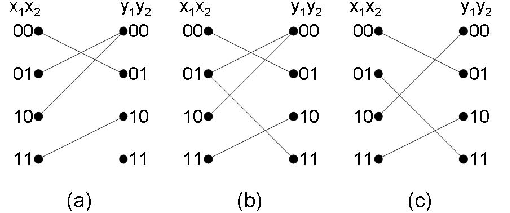
\includegraphics[width=0.8\textwidth]{relation}
\end{center}
\caption{关系和函数的布尔映射}
  \label{fig_relation}
\end{figure}

为此,
我们在本章中提出了基于余因子和Craig插值的迭代特征化算法,
以从布尔关系$R(\vec{a},\vec{b},t)$中特征化函数$t=f(\vec{a})$。

在本章中,
我们首先在小节\ref{sec_craigimp}描述Craig插值的基本原理,
然后在小节\ref{sec_craigchar}中将其应用至一种受限的特殊情况下以求解特征化函数。
最后在小节\ref{sec_iterativecraig}中将其扩展到包含额外变量$\vec{c}$ 的更一般情形$R(\vec{a},\vec{b},\vec{c})$。

\section{Craig插值的原理和实现}\label{sec_craigimp}
注意本小节描述的Craig插值原理不是我们的原创,
而是为了方便上下文的叙述从\upcite{DBLP:conf/cav/McMillan03} 移植至此。
\subsection{相关背景知识和记法}
在通常的SAT求解器,
包括本文使用的MiniSat\upcite{EXTSAT}中,
要求待求解的公式被表示为CNF格式。
其中一个公式是多个短句的合取(conjunction),
而每一个短句是多个文字的析取(disjunction),
而每个文字是一个布尔变量$v$或者其反$\neg v$。
如公式$(v_0\vee\neg v_1\vee v_2)\wedge(v_1\vee v_2)\wedge(\neg v_0\vee v_2)$,
包含短句$v_0\vee\neg v_1\vee v_2$,$v_1\vee v_2$和$\neg v_0\vee v_2$。
而短句$v_0\vee\neg v_1\vee v_2$包含文字$v_0$, $\neg v_1$和$v_2$。

当存在一个变量$v$,
使得一个短句$c$中同时包含两个文字$v$和$\neg v$,
则称$c$为tautological的。
我们通常假设有待SAT求解器求解的公式中所有的短句都是非tautological的。

假设公式$F$的布尔变量全集为$V$。
若存在对$V$的赋值函数$A:V\to \{0,1\}$,
使得$F$中的每个短句均能取值为1,
则称$F$是可满足的,
此时SAT求解器能够找到赋值函数$A$。
否则称$F$为不可满足的,
此时SAT求解器能够产生如下一小节所述的不可满足证明。

\subsection{不可满足证明}
对于两个短句$c_1=v\vee B$和$c_2=\neg v\vee C$,
当$A\vee B$是非tautological的时,
$A\vee B$称为他们的resolvant。
而$v$称为他们的pivot。
易知以下事实:

\begin{equation}
\begin{array}{ccc}
&resolvant(c_1,c_2) = \exists v, c_1\wedge c_2 &\\
&c_1\wedge c_2 \to resolvant(c_1,c_2)&
\end{array}
\end{equation}

\begin{definition}
对于不可满足公式$F$,
假设其短句集合为$C$,
则其不可满足证明$\Pi$是一个有向无环图$(V_{\Pi},E_{\Pi})$,
其中$V_{\Pi}$是短句集合,
而$E_{\Pi}$是链接$V_{\Pi}$中节点的边集合。
$\Pi$满足如下要求:
\begin{enumerate}
\item 对于节点$c\in V_{\Pi}$:
  \begin{enumerate}
    \item 要么$c\in C$,此时称$c$为$\Pi$的根
    \item 或者$c$有且仅有两个predecessors $c_1$和$c_2$,
    使得$c$是$c_1$和$c_2$的resolvant。
  \end{enumerate}
\item 空短句是$\Pi$的唯一一个叶节点。
\end{enumerate}
\end{definition}

直观的说,
$\Pi$就是一棵树,
以短句集合$C$的子集为根,
以空短句为唯一叶节点。
而每个节点的两个扇入边代表了一个resolving关系。

包括本文使用的MiniSat求解器\upcite{EXTSAT}在内的许多SAT求解器,
当公式不可满足时都将产生一个不可满足证明$\Pi$。

\subsection{Craig插值算法}

根据文献\upcite{Craig},
给定两个布尔逻辑公式$A$ 和$B$,
若$A\wedge B$ 不可满足,
则存在仅使用了$A$ 和$B$共同变量的公式$I$ ,
使得$A\Rightarrow I$且
$I\wedge B$不可满足。
$I$ 被称为$A$针对$B$的Craig插值\upcite{Craig}。

目前最常见且最高效的产生Craig插值的算法是
McMillan算法\upcite{interp_McMillan} 。
其基本原理描述如下。

对于上述公式$A$和$B$,
已知$A\cup B$不可满足,
而$\Pi$是SAT求解器给出的不可满足证明。
当一个变量$v$同时出现在$A$和$B$中时,
我们称其为全局变量。
若$v$只出现在$A$中,
则称其为$A$本地变量。

对于文字$v$或者$\neg v$,
当变量$v$是全局变量或者$A$本地变量时,
称该文字为全局文字或者$A$本地文字。

对于短句$c$,
令$g(c)$为$c$中所有全局文字的析取,
而$l(c)$为$c$中所有$A$本地文字的析取。

例如,
假设有两个短句$c_1=(a\vee b\vee\neg c)$ 和
$c_2=(b\vee c\vee\neg d)$。
并假设$A=\{c_1\}$和$B=\{c_2\}$。
则$g(c_1)=(b\vee\neg c)$,
$l(c_1)=(a)$,
$g(c_2)=(b\vee c)$,
$l(c_2)=FALSE$。


\begin{definition}\label{def_gencraig}
令$(A,B)$为一对公式,
而$\Pi$是$A\cup B$的不可满足证明,
且其唯一叶节点是空短句$FALSE$。
对于每一个节点$c\in V_{\Pi}$,
令$p(c)$为如下定义的一个公式:
\begin{enumerate}
\item 如果$c$是根节点则
  \begin{enumerate}
    \item 如果$c\in A$则$p(c)=g(c)$
    \item 否则$p(c)=TRUE$
  \end{enumerate}
\item 否则令$c_1$和$c_2$分别是$c$的两个扇入节点,而$v$是他们的pivot变量
  \begin{enumerate}
    \item 如果$v$是$A$本地变量,则$p(c)=p(c_1)\vee p(c_2)$。
    \item 否则$p(c)=p(c_1)\wedge p(c_2)$。
  \end{enumerate}
\end{enumerate}
\end{definition}

上述定义\ref{def_gencraig}是构造性的,
已经给出了从$\Pi$得到最终的插值的算法,
即以$\Pi$的根节点为起点,
为每一个$c$计算相应的$p(c)$,
直至到达最终的唯一叶节点$FALSE$。
我们有以下定理:

\begin{theorem}
定义\ref{def_gencraig}为唯一叶节点$FALSE$产生的$p(FALSE)$即为
$A$相对于$B$的Craig插值。
\end{theorem}

该定理的详细证明可见文献\upcite{DBLP:journals/tcs/McMillan05}。

计算$A$相对于$B$的Craig插值的时间复杂性为$O(N+L)$,
其中$N$是$\Pi$中包含的节点个数$|V_{\Pi}|$,
而$L$是$\Pi$中的文字个数$\sigma_{c\in V_{\Pi}}|c|$。
而所产生的插值可以视为一个电路,
其空间复杂性为$|O(N+L)|$。
当然,
$\Pi$的尺寸在最坏情况下也是$A\cup B$的尺寸的指数。



\section{非迭代的特征化算法}\label{sec_craigchar}

假设有布尔关系$R(t,\vec{a})$使得
$R(1,\vec{a})\wedge R(0,\vec{a})$不可满足。
而我们需要从$R$中特征化函数$f$,
使得$t=f(\vec{a})$。
则根据上述的讨论,
可以简单的令$A=R(1,\vec{a})$而$B=R(0,\vec{a})$。
此时$A$相对于$B$的Craig插值$\Pi$具有以下性质:

\begin{enumerate}
\item $R(1,\vec{a})\to \Pi$,这说明$\Pi$覆盖了所有能够使得$R(1,\vec{a})$的$\vec{a}$。
\item $R(0,\vec{a})\wedge \Pi$不可满足,这说明$\Pi$没有覆盖任何使得$R(0,\vec{a})$的$\vec{a}$。
\item $\Pi$仅引用了$R(0,\vec{a})$和$R(1,\vec{a})$的共同变量集合$\vec{a}$。这说明$\Pi$是一个定义在$\vec{a}$上的函数。
\end{enumerate}

因此,
$\Pi$即为函数$f$。

该算法在本文的后继章节中被广泛应用于构造解码器的布尔函数。


\section{迭代的特征化算法}\label{sec_iterativecraig}
上一小节讨论了如何从关系$R(a,\vec{b})$特征化函数$a=f(\vec{b})$。
然而在更一般的情形下,我们需要从$R(\vec{a},\vec{b},t)$特征化函数$t=f(\vec{a})$。
相比之下,此时多了一个需要进行存在性量化的$\vec{b}$。
为此我们需要将上述算法进行以下扩展。

假设$R(\vec{a},\vec{b},t)$是一个使得$R(\vec{a},\vec{b},0)\wedge R(\vec{a},\vec{b},1)$ 不可满足的布尔公式。

其中$\vec{a}$ 和$\vec{b}$ 被分别称为重要和非重要变量子集。
而$t$ 是目标变量。
我们进一步假设$R(\vec{a},\vec{b},t)$ 是可满足的。

我们需要特征化一个布尔函数$FSAT_R(\vec{a})$,
覆盖且仅覆盖了所有能够使得$R(\vec{a},\vec{b},1)$ 可满足的$\vec{a}$。
形式化的定义是:

\begin{equation}\label{fchar}
% \begin{split}
FSAT_R(\vec{a}):=
\left\{
\begin{array}{rcl}
1 & & \exists\vec{b}.R(\vec{a},\vec{b},1) \\
0 & & otherwise
\end{array}
\right.
% \end{split}
\end{equation}
%% HAHA come to here

因此,
一个计算$FSAT_R(\vec{a})$ 的简单算法是:
逐一遍历并收集所有使得$R(\vec{a},\vec{b},1)$ 可满足的$\vec{a}$的赋值。
然而该算法需要处理$2^{|\vec{a}|}$中情况。
对于很长的$\vec{a}$,时间开销将会很大。

使用cofactoring \upcite{EFFSATUSMCCO} 和Craig 插值\upcite{interp_McMillan},
可以将每一个$\vec{a}$ 扩展为一个更大的集合,
从而极大的提高算法运行速度。
直观的,
假设$R(\vec{a},\vec{b},1)$ 的一个满足赋值是$A:\vec{a}\cup\vec{b}\cup\{t\}\to\{0,1\}$,
通过cofactoring\upcite{EFFSATUSMCCO}可以构造以下公式:

\begin{algorithm}[t]
\caption{$CharacterizingFormulaSAT(R,\vec{a},\vec{b},t)$: 特征化使得$R(\vec{a},\vec{b},1)$ 可满足的$\vec{a}$ 集合}
\label{alg_craigchar}
%\KwIn{The Boolean formula $R(\vec{a},\vec{b},t)$,
%its important variable vector $\vec{a}$,
%its non-important variable vector $\vec{b}$,
%and its target variable $t$.}
%\KwOut{$FSAT_R(\vec{a})$ that makes $R(\vec{a},\vec{b},1)$ satisfiable.}
\begin{algorithmic}[1]
\label{initcondition}
\STATE $FSAT_R(\vec{a}):= 0$ ;
\WHILE { $R(\vec{a},\vec{b},1)\wedge\neg FSAT_R(\vec{a})$ 是可满足的}
\label{testsat}
  \STATE 假设 $A:\vec{a}\cup\vec{b}\cup\{t\}\rightarrow \{0,1\}$ 可满足赋值函数;
  \STATE $\phi_A(\vec{a}):= R(\vec{a},A(\vec{b}),1)$ ;
\label{cofact1}
  \STATE $\phi_B(\vec{a}):= R(\vec{a},A(\vec{b}),0)$ ;
\label{cofact2}
  \STATE 假设 $ITP(\vec{a})$ 是$\phi_A$ 针对$\phi_B$的Craig插值 ;
\label{ab}
  \STATE $FSAT_R(\vec{a}):= ITP(\vec{a}) \vee FSAT_R(\vec{a})$ ;
\label{add}
\ENDWHILE
\RETURN $FSAT_R(\vec{a})$
\end{algorithmic}
\end{algorithm}

\begin{equation}
% \begin{split}
R(\vec{a},A(\vec{b}),1):=R(\vec{a},\vec{b},1)_{b\equiv A(b)}
% \end{split}
\end{equation}

因为$R(\vec{a},A(\vec{b}),0)\wedge R(\vec{a},A(\vec{b}),1)$ 是不可满足的,
$R(\vec{a},A(\vec{b}),1)$针对$R(\vec{a},A(\vec{b}),0)$的Craig插值$ITP(\vec{a})$ 可以用作$\vec{a}$ 使得$R(\vec{a},A(\vec{b}),1)$ 可满足的上估计。
同时,
$ITP(\vec{a})\wedge R(\vec{a},A(\vec{b}),0)$ 是不可满足的,
因此$ITP(\vec{a})$ 没有覆盖任何使得$R(\vec{a},A(\vec{b}),0)$ 可满足的情况。
因此,
$ITP(\vec{a})$ 覆盖且仅覆盖了所有使得$R(\vec{a},A(\vec{b}),1)$ 可满足的$\vec{a}$。


基于上述讨论,
我们提出了算法\ref{alg_craigchar} 以特征化等式(\ref{fchar})中的$FSAT_R(\vec{a})$。
行\ref{testsat}检测是否仍然存在尚未被$FSAT_R(\vec{a})$覆盖的$\vec{a}$ ,
使得$R(\vec{a},\vec{b},1)$ 可满足。
行\ref{cofact1} 和\ref{cofact2} 将可满足赋值中$\vec{b}$的取值分别赋予
$R(\vec{a},\vec{b},1)$ 和$R(\vec{a},\vec{b},0)$ 。
这将使得$\vec{b}$ 不在出现在这两个公式中。

因此,
$\phi_A\wedge \phi_B$ 在行\ref{ab} 是不可满足的。
且$\phi_A$ 和$\phi_B$ 的共同变量是$\vec{a}$。
因此可以使用McMillian算法\upcite{interp_McMillan} 计算Craig 插值$ITP(\vec{a})$。

$ITP(\vec{a})$ 将在行\ref{add}被加入$FSAT_R(\vec{a})$  并在行\ref{testsat} 被排除。

算法\ref{alg_craigchar} 的每一个循环将向$FSAT_R(\vec{a})$ 中加入至少一个$\vec{a}$ 的赋值。
这意味着$FSAT_R(\vec{a})$ 覆盖了$\vec{a}$的一个有界并且单调增长的赋值集合。
因此算法\ref{alg_craigchar} 是停机的。

\section{可选的BDD整理和化简}

上述由迭代特征化算法产生的函数,
本质上是一系列Craig插值结果的析取。
然而,
正如小节\ref{sec_craigchar}所指出的,
Craig插值结果是一个包含大量自由组合的与门和或门的电路,
结构非常不规则。

因此,
我们提出了基于BDD的整理算法。
利用BDD本身的规范性(canonical),
将Craig插值结果转换为BDD,
并直接导出为多个合取项的析取形式。

该算法能够极大的化简Craig插值结果的表达式。
因此通常用于特征化下一章的控制流谓词。


\section{本章小结}
本章综述了Craig插值算法的原理及其实现,
以及基于该实现的迭代是特征化算法。
这些算法将在本文的剩余部分被其他算法频繁调用。



% !Mode:: "Tex:UTF-8"
\chapter{面向流控机制和流水线的对偶综合}
\label{chap:4}

\section{引言}\label{sec_intro}
在通讯和多媒体芯片设计项目中,
一个最困难的工作之一是为不同的协议设计编码器和解码器。
其中编码器负责将输入向量$\vec{i}$ 映射到输出向量$\vec{o}$,
而解码器负责从$\vec{o}$中恢复$\vec{i}$。
对偶综合\cite{ShenICCAD09,ShenTCAD11,ShenTCAD12,LiuICCAD11,LiuTCAD12,TuDAC13}
假设$\vec{i}$ 总能够被 $\vec{o}$唯一决定,
并自动产生相应的解码器。

然而,
许多编码器中采用的留空机制\cite{flowcontrol}
不能满足该要求。
如图\ref{fig_fc}a)所示,
当接收器无法跟上发送器时,
该机制通过发送空闲字符$I$ 以防止快速发送器充爆慢速接收器。
如图\ref{fig_fc}b)所示,
空闲字符$I$
只能唯一决定$\vec{i}$的一部分而非全部,
我们称之为流控向量$\vec{f}$。
而正常的编码结果$D_i$ 能
唯一决定所有输入
包括流控向量$\vec{f}$ 和数据向量$\vec{d}$。

秦et al. \cite{QinTODAES15} 首次提出了能够处理流控机制的对偶综合算法。
该算法首先找到所有的能够被$\vec{o}$唯一决定的$i\in\vec{f}$。
然后推导一个能使得$\vec{d}$ 被$\vec{o}$唯一决定的谓词$valid(\vec{f})$。

\begin{figure}[t]
\centering
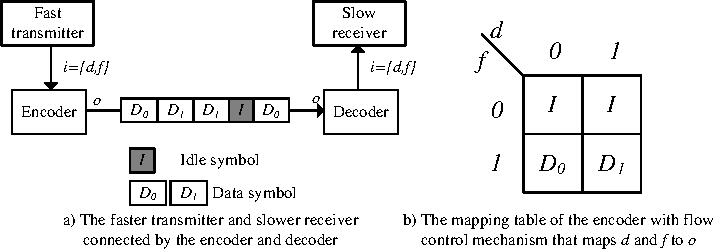
\includegraphics[width=\textwidth]{nonuniq_pred}
\caption{带有流控机制的编码器}
\label{fig_fc}
\end{figure}

\begin{figure}[b]
\centering
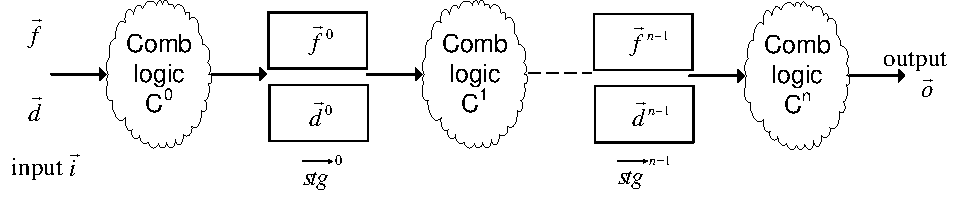
\includegraphics[width=0.9\textwidth]{pipemod1_pred}
\caption{带有流水线和流控机制的编码器}
\label{pipemod}
\end{figure}



同时,
如图\ref{pipemod}所示,
许多编码器
包含流水线级$\vec{stg}^j$ 已将关键的数据路径划分为多个子段$C^j$,
这样有助于提高性能。
类似于$\vec{i}$,
每个流水线级$\vec{stg}^j$ 也可以划分为留空向量$\vec{f}^j$ 和数据向量$\vec{d}^j$。

然而由秦et al. 的算法\cite{QinTODAES15} 产生的解码器并不包含流水线。
这使得其运行速度远低于相应的编码器。
为了解决该问题,
本文提出了一个全新的算法以为此类编码器产生带有流控机制和流水线的解码器。
该算法首先使用秦et al. \cite{QinTODAES15}的算法来寻找$\vec{f}$ 并推导$valid(\vec{f})$。
然后分别通过强制和不强制$valid(\vec{f})$,
已从所有寄存器集合中找到每一个寄存器级$\vec{stg}^j$的$\vec{d}^j$ 和$\vec{f}^j$。
最后通过Jiang et al. \cite{InterpBoolFunction}的算法特征化$\vec{stg}^j$ 和$\vec{i}$的布尔函数。

实验结果表明,
该算法能够为多个工业界的真实编码器正确的产生带有流控和流水线的解码器。

本文剩余部分如下组织。
小节\ref{sec_prem} 介绍相关的背景知识;
小节\ref{sec_framework} 介绍本文算法的整体结构;
小节\ref{sec_pipeinfer} 找到每一个流水线级$\vec{stg}^j$中的$\vec{f}^j$ 和$\vec{d}^j$ 。
小节\ref{sec_char} 为$\vec{stg}^j$ 和$\vec{i}$特征化布尔函数。
小节\ref{sec_exp} 和\ref{sec_relwork} 分别给出实验结果和相关工作。
最后小节\ref{sec_conclude} 给出结论。


\section{背景知识}\label{sec_prem}

% \subsection{Flow control mechanism}\label{subsec_fc}



\subsection{命题逻辑可满足}\label{subsec_SAT}
布尔集合记为$\mathbb{B}=\{0,1\}$。
多个变量组成的向量记为$\vec{v}=(v,\dots)$。
$\vec{v}$ 中的变量个数记为$|\vec{v}|$。
若一个变量$v$ 是$\vec{v}$的成员,
则记为$v\in\vec{v}$;
否则记为$v\notin\vec{v}$。
对于一个变量$v$ 和一个向量$\vec{v}$,
若$v\notin\vec{v}$,
则一个同时包含$v$ 和所有$\vec{v}$ 的成员的新变量记为$v\cup\vec{v}$。
若$v\in \vec{v}$,
则一个包含$\vec{v}$ 的所有成员,但是不包含$v$的
新变量记为$\vec{v}-v$。
对于两个向量$\vec{a}$ 和$\vec{b}$,
则同时包含$\vec{a}$ 和$\vec{b}$ 的所有成员的新向量记为$\vec{a}\cup\vec{b}$。

对于变量集合$V$上的公式$F$,
其命题逻辑可满足问题(SAT)
的目的在于巡展赋值函数$A:V\to \mathbb{B}$,
使得$F$ 能够取值为$1$。
若$A$ 存在则$F$ 是可满足的;
否则是不可满足的。

对于两个布尔命题逻辑公式$\phi_A$ 和$\phi_B$,
若$\phi_A\wedge \phi_B$ 不可满足,
则存在仅引用$\phi_A$ 和$\phi_B$共同变量的公式$\phi_I$ ,
使得$\phi_A\Rightarrow \phi_I$
且$\phi_I\wedge \phi_B$ 不可满足。
$\phi_I$ 称为$\phi_A$ 相对于$\phi_B$的Craig 插值\cite{Craig} 。
可以使用McMillan算法 \cite{interp_McMillan} 产生该插值。




\subsection{有限状态机}\label{subsec_fsm}



编码器使用有限状态机$M=(\vec{s},\vec{i},\vec{o},T)$作为模型,
其中包含状态向量$\vec{s}$。
输入向量$\vec{i}$,
输出向量$\vec{o}$,
状态迁移函数$T: \vec{s}\times \vec{i}\to \vec{s}\times \vec{o}$
从当前状态向量和输入向量计算出下一状态向量和输出向量。

$M$ 的行为可以通过展开状态迁移函数进行推导。
状态变量$s\in\vec{s}$, 输入变量$i\in\vec{i}$ 和输出变量$o\in\vec{o}$ 在上述展开序列的第$n$步中
分别记为$s_n$, $i_n$ 和$o_n$。
更进一步的,
在第$n$步中的状态向量,输入向量和输出向量分别记为$\vec{s}_n$, $\vec{i}_n$ 和$\vec{o}_n$。
一个路径是一个序列$<\vec{s}_n,\dots,\vec{s}_m>$ 使得对于所有$n\le j< m$,
有$\exists \vec{i}_j\vec{o}_j (\vec{s}_{j+1},\vec{o}_j)\equiv T(\vec{s}_j,\vec{i}_j)$ 。
而一个环是一个路径$<\vec{s}_n,\dots,\vec{s}_m>$ 使得$\vec{s}_n\equiv \vec{s}_m$。



\subsection{寻找$\vec{f}$的停机算法}\label{subsec_chkextdec}


秦et al. \cite{QinTODAES15} 提出了一个寻找$\vec{f}$ 的停机算法。
该算法通过迭代的调用一个sound和一个complete的算法以最终得到收敛的答案。.
% The first one is an under-approximative one that presented in \ref{subsub_sound},
% while the second one is an over-approximative one presented in \ref{subsub_complete}.
% We will present these two approaches below and show
% that they will eventually converge.

\subsubsection{sound算法}\label{subsub_sound}
如图\ref{fig_pc}a)所示,
在展开的迁移关系上,
一个输入变量$i\in\vec{i}$ 能够被唯一决定,
是指存在$p$, $l$ 和$r$,
使得对于输出序列$<\vec{o}_p,\dots,\vec{o}_{p+l+r}>$的每一个取值,
$i_{p+l}$ 不能同时为0和1。
折等价于公式(\ref{uniqt1})中的$F_{PC}(p,l,r)$的不可满足性。
行1 对应于图\ref{fig_pc}a)中的路径,
而行2 是其拷贝
行3 强制这两个路径的输出相等。
而行4 强制$i_{p+l}$ 不等。
该算法是sound的因为当(\ref{uniqt1}) 不可满足
$i$ 肯定是$\vec{f}$的成员。

\begin{equation}\label{uniqt1}
% \begin{split}
F_{PC}(p,l,r):=
\left\{
\begin{array}{cc}
&\bigwedge_{m=0}^{p+l+r}
\{
(\vec{s}_{m+1},\vec{o}_m)\equiv T(\vec{s}_m,\vec{i}_m)
\}
\\
\wedge&\bigwedge_{m=0}^{p+l+r}
\{
(\vec{s'}_{m+1},\vec{o'}_m)\equiv T(\vec{s'}_m,\vec{i'}_m)
\}
\\
\wedge&\bigwedge_{m=p}^{p+l+r}\vec{o}_m\equiv \vec{o'}_m \\
\wedge& i_{p+l}\equiv 1 \wedge  i'_{p+l}\equiv 0
% \wedge&\bigwedge_{m=0}^{p+l+r}assertion(\vec{i}_m) \\
% \wedge&\bigwedge_{m=0}^{p+l+r}assertion(\vec{i'}_m)
\end{array}
\right\}
% \end{split}
\end{equation}

\begin{figure}[t]
\begin{center}
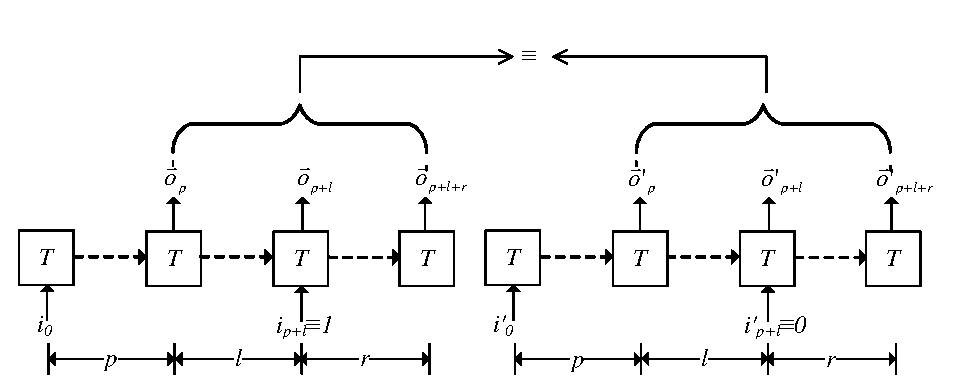
\includegraphics[width=\textwidth]{pc}
\end{center}
\caption{sound和complete方法}
  \label{fig_pc}
\end{figure}


%



\subsubsection{complete算法}\label{subsub_complete}
对于上述的$F_{PC}(p,l,r)$ ,
有两种可能性:
\textbf{(1)}. 存在$p$, $l$ 和$r$,使得$i_{p+l}$ 能够被$<\vec{o}_{p},\dots,\vec{o}_{p+l+r}>$ 唯一决定;
或者\textbf{(2)}. $i_{p+l}$ 对于任意$p$, $l$ 和$r$都不能被唯一决定。


对于第一种情形,
通过迭代的增加$p$, $l$ 和$r$,
$F_{PC}(p,l,r)$ 总能够变成不可满足。
而对于第二种情形,
该算法将永不停机。
因此,
为了得到一个停机算法,
我们需要如图\ref{fig_pc}b) 所示的方法去检查第二种情形。
该方法类似于\ref{fig_pc}a) ,
但是在三个状态序列$<\vec{s}_{0},\dots,\vec{s}_{p}>$, $<\vec{s}_{p+1},\dots,\vec{s}_{p+l}>$ 和
$<\vec{s}_{p+l+1},\dots,\vec{s}_{p+l+r}>$上增加了三个约束用于检测环。
该方法形式化的定义于公式(\ref{uniqln})中。
其中最后三行即为我们新加的三个约束。
该方法是complete,
因为当其是可满足的时候,
我们可以通过展开
这三个环来证明第二种情形并断定 $i\notin \vec{f}$。

\begin{equation}\label{uniqln}
% \begin{split}
F_{LN}(p,l,r):=\\
\left\{
\begin{array}{cc}
&F_{PC}(p,l,r)\\
\wedge&\bigvee_{x=0}^{p-1}\bigvee_{y=x+1}^{p} \{\vec{s}_x\equiv \vec{s}_y\wedge \vec{s'}_x\equiv \vec{s'}_y\} \\
\wedge&\bigvee_{x=p+1}^{p+l-1}\bigvee_{y=x+1}^{p+l} \{\vec{s}_x\equiv \vec{s}_y\wedge \vec{s'}_x\equiv \vec{s'}_y\} \\
\wedge&\bigvee_{x=p+l+1}^{p+l+r-1}\bigvee_{y=x+1}^{p+l+r} \{\vec{s}_x\equiv \vec{s}_y\wedge \vec{s'}_x\equiv \vec{s'}_y\}
\end{array}
\right\}
% \end{split}
\end{equation}


\subsubsection{通过算法\ref{alg_fofc}找到$\vec{f}$ }\label{subsubsec_findfc}

在行\ref{adduniq},
所有能够被唯一决定的输入$i$ 将被移到$\vec{f}$。
若$F_{LN}(p,l,r)$ 在行\ref{nonuniqres}是可满足的,
所有可满足的输入$i$ 将被移到$\vec{d}$.
该算法的正确性和停机性证明请见\cite{QinTODAES15} 。

\begin{algorithm}[t]
\begin{algorithmic}[1]
\STATE{输入:输入向量$\vec{i}$.}
\STATE{输出:$\vec{f}\subset \vec{i}$, 在此次搜索中找到的最大$p$, $l$ 和$r$ }
\STATE $\vec{f}: = \{\}$;$\vec{d}:= \{\}$;$p$:= 0 ;~$l$:= 0 ;~$r$:= 0 \;
\label{while}\WHILE{$\vec{i}\ne \{\}$}
  \STATE 假设$i\in\vec{i}$\;
  \STATE $p++$; ~ $l++$; ~ $r++$\;
  \IF {$F_{PC}(p,l,r)$ 对于$i$不可满足} 
    \label{adduniq}
    \STATE $\vec{f}:= i\cup\vec{f}$ ; ~
    \STATE $\vec{i}:=\vec{i}-i$\;
  \label{nonuniqres}
  \ELSIF {$F_{LN}(p,l,r)$ 对于$i$可满足}
    \STATE $\vec{d}:=i\cup\vec{d}$ ; ~
    \STATE $\vec{i}:=\vec{i}-i$
  \ENDIF
\ENDWHILE
\RETURN ($\vec{f}$, $p$, $l$, $r$)
\caption{Identifying the flow control vector $\vec{f}$}
\label{alg_fofc}
\end{algorithmic}
\end{algorithm}





\subsection{推导使得$\vec{d}$ 被唯一决定的$valid(\vec{f})$ }\label{subsec_infer}

该算法也是由秦et al. \cite{QinTODAES15}提出的。
它首先给出算法\ref{alg_craigchar},
该算法用于特征化一个函数,覆盖所有能够使得一个布尔关系满足的赋值集合。
然后如图\ref{fig_mono}所示,
算法\ref{alg_craigchar} 被用于特征化函数$\neg FSAT_{PC}(p,l,r)$,
$valid(\vec{f})$的单调递增下估计,
和$\neg FSAT_{LN}(p,l,r)$,
$valid(\vec{f})$的单调递减上估计。
最终我们指出这两者将收敛到$valid(\vec{f})$。
% Please refer to \cite{QinTODAES15} for the proof of its correctness and termination.



\subsubsection{特征化使得一个布尔关系可满足的布尔函数}\label{subsubsec_craig}

对于一个布尔关系$R(\vec{a},\vec{b},t)$,
有$R(\vec{a},\vec{b},0)\wedge R(\vec{a},\vec{b},1)$ 不可满足。
算法\ref{alg_craigchar} 特征化一个布尔寒素$FSAT_R(\vec{a})$,
该函数覆盖且仅覆盖了能使得
$R(\vec{a},\vec{b},1)$ 可满足的所有$\vec{a}$。
行\ref{testsat} 找到$\vec{a}$ 的一个赋值,
尚未被 $FSAT_R(\vec{a})$ 覆盖而且能够使得$R(\vec{a},\vec{b},1)$ 可满足。
行\ref{cofact1}, \ref{cofact2} 和\ref{ab} 使用
McMillan算法\cite{interp_McMillan} 将该赋值放大为$ITP(\vec{a})$。
行\ref{add} 将$ITP(\vec{a})$ 加入$FSAT_R(\vec{a})$。


\begin{algorithm}[t]
\begin{algorithmic}[1]
\STATE{输入:布尔关系$R(\vec{a},\vec{b},t)$}
\STATE{输出:能够使得$R(\vec{a},\vec{b},1)$ 可满足的$FSAT_R(\vec{a})$ }
\label{initcondition}
\STATE $FSAT_R(\vec{a}):= 0$ ;
\label{testsat}
\WHILE { $R(\vec{a},\vec{b},1)\wedge\neg FSAT_R(\vec{a})$ 可满足} 
  \STATE 假设$A:\vec{a}\cup\vec{b}\cup\{t\}\rightarrow \{0,1\}$ 是一个可满足赋值;
\label{cofact1}
  \STATE $\phi_A(\vec{a}):= R(\vec{a},A(\vec{b}),1)$ ;
\label{cofact2}
  \STATE $\phi_B(\vec{a}):= R(\vec{a},A(\vec{b}),0)$ ;
\label{ab}
  \STATE 假设$ITP(\vec{a})$ 是$\phi_A$ 相对于$\phi_B$ 的Craig插值 ;
\label{add}
  \STATE $FSAT_R(\vec{a}):= ITP(\vec{a}) \vee FSAT_R(\vec{a})$ ;
\ENDWHILE
\RETURN $FSAT_R(\vec{a})$
\caption{$CharacterizingFormulaSAT(R,\vec{a},\vec{b},t)$}
\label{alg_craigchar}
\end{algorithmic}
\end{algorithm}

\subsubsection{计算$valid(\vec{f})$的单调递增下估计}\label{subsub_nonloop}
通过将公式(\ref{uniqt1}) 中的$i$替换为算法\ref{alg_fofc}中推导的$\vec{d}$ ,
我们有:

\begin{equation}\label{uniqt1d}
% \begin{split}
F^d_{PC}(p,l,r):=
\left\{
\begin{array}{cc}
&\bigwedge_{m=0}^{p+l+r}
\{
(\vec{s}_{m+1},\vec{o}_m)\equiv T(\vec{s}_m,\vec{i}_m)
\}
\\
\wedge&\bigwedge_{m=0}^{p+l+r}
\{
(\vec{s'}_{m+1},\vec{o'}_m)\equiv T(\vec{s'}_m,\vec{i'}_m)
\}
\\
\wedge&\bigwedge_{m=p}^{p+l+r}\vec{o}_m\equiv \vec{o'}_m \\
\wedge& \vec{d}_{p+l}\ne \vec{d}'_{p+l} \\
% \wedge&\bigwedge_{m=0}^{p+l+r}assertion(\vec{i}_m) \\
% \wedge&\bigwedge_{m=0}^{p+l+r}assertion(\vec{i'}_m)
\end{array}
\right\}
% \end{split}
\end{equation}

% Here,
% $\vec{d}_{p+l}\ne \vec{d}'_{p+l}$ means some bit in $\vec{d}_{p+l}$
% isn't equal to the corresponding bit in $\vec{d}'_{p+l}$.
若$F^d_{PC}(p,l,r)$ 可满足,
则$\vec{d}_{p+l}$ 不能被$<\vec{o}_p,\dots,\vec{o}_{p+l+r}>$唯一决定。
通过收集公式 (\ref{uniqt1d})的第三行,
我们定义$T_{PC}(p,l,r)$ :

\begin{equation}\label{tpc}
% \begin{split}
T_{PC}(p,l,r):=\\
\left\{
\begin{array}{cc}
      &\bigwedge_{m=p}^{p+l+r}\vec{o}_m\equiv \vec{o'}_m \\
\end{array}
\right\}
% \end{split}
\end{equation}

\begin{figure}[b]
\begin{center}
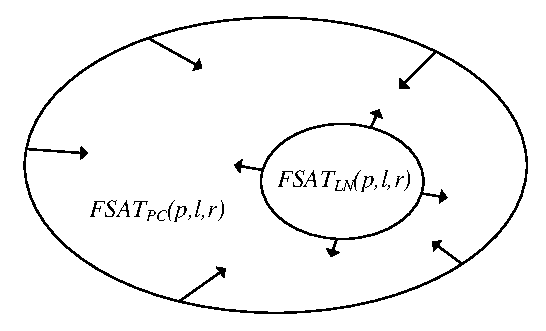
\includegraphics[width=0.5\textwidth]{mono}
\end{center}
\caption{The monotonicity of $FSAT_{PC}(p,l,r)$ and $FSAT_{LN}(p,l,r)$}
  \label{fig_mono}
\end{figure}

通过将$T_{PC}(p,l,r)$ 替换回$F^d_{PC}(p,l,r)$,
我们有:

\begin{equation}\label{fpcq}
% \begin{split}
F'^d_{PC}(p,l,r,t):=
\left\{
\begin{array}{cc}
&\bigwedge_{m=0}^{p+l+r}
\{
(\vec{s}_{m+1},\vec{o}_m)\equiv T(\vec{s}_m,\vec{i}_m)
\}
\\
\wedge&\bigwedge_{m=0}^{p+l+r}
\{
(\vec{s'}_{m+1},\vec{o'}_m)\equiv T(\vec{s'}_m,\vec{i'}_m)
\}
\\
\wedge& t\equiv T_{PC}(p,l,r)\\
\wedge& \vec{d}_{p+l}\ne \vec{d'}_{p+l} \\
% \wedge&\bigwedge_{m=0}^{p+l+r}assertion(\vec{i}_m) \\
% \wedge&\bigwedge_{m=0}^{p+l+r}assertion(\vec{i'}_m)
\end{array}
\right\}
% \end{split}
\end{equation}


很明显$F^d_{PC}(p,l,r)$ 和$F'^d_{PC}(p,l,r,1)$ 是等价的,
我们进一步定义:

\begin{equation}\label{pcdef1}
\vec{a}:=\vec{f}_{p+l}
\end{equation}

\begin{equation}\label{pcdef2}
\vec{b}:=\vec{d}_{p+l}\cup \vec{d'}_{p+l}\cup \vec{s}_0\cup \vec{s'}_0\cup\bigcup_{0\le x\le p+l+r,x\neq (p+l)}(\vec{i}_{x}\cup\vec{i'}_{x})
\end{equation}

因此,
向量$\vec{a}\cup\vec{b}$ 包含所有步的输入向量$<\vec{i}_0,\dots,\vec{i}_{p+l+r}>$ 和$<\vec{i'}_0,\dots,\vec{i'}_{p+l+r}>$。
它同时也包含两个初始状态$\vec{s}_0$ 和$\vec{s'}_0$。
因此$\vec{a}$ 和$\vec{b}$ 能唯一决定$F'^d_{PC}(p,l,r,t)$中$t$ 的取值。
这意味着$R(\vec{a},\vec{b},1)\wedge R(\vec{a},\vec{b},0)$ 是不可满足的。
因此,
对于$p$, $l$ 和$r$的特定组合,
在$\vec{f}_{p+l}$ 上定义且能够使$F'^d_{PC}(p,l,r,1)$ 满足的函数可以通过使用$F'^d_{PC}(p,l,r,t)$, $\vec{a}$ 和$\vec{b}$ 调用算法定义如下:

\begin{equation}\label{fsat_pc}
FSAT_{PC}(p,l,r):=CharacterizingFormulaSAT(F'^d_{PC}(p,l,r,t),\vec{a},\vec{b},t)
\end{equation}

如图\ref{fig_mono}所示,
$\neg FSAT_{PC}(p,l,r)$ 是$valid(\vec{f})$ 的针对
$p$, $l$ 和$r$
单调递增的下估计。
% \end{proposition}




\subsubsection{计算$valid(\vec{f})$的单调递减上估计}\label{subsub_loop}
类似的,
我们定义:

\begin{equation}\label{tln}
% \begin{split}
T_{LN}(p,l,r):=\\
\left\{
\begin{array}{cc}
      &\bigwedge_{m=p}^{p+l+r}\vec{o}_m\equiv \vec{o'}_m \\
\wedge&\bigvee_{x=0}^{p-1}\bigvee_{y=x+1}^{p} \{\vec{s}_x\equiv \vec{s}_y\wedge \vec{s'}_x\equiv \vec{s'}_y\} \\
\wedge&\bigvee_{x=p+1}^{p+l-1}\bigvee_{y=x+1}^{p+l} \{\vec{s}_x\equiv \vec{s}_y\wedge \vec{s'}_x\equiv \vec{s'}_y\} \\
\wedge&\bigvee_{x=p+l+1}^{p+l+r-1}\bigvee_{y=x+1}^{p+l+r} \{\vec{s}_x\equiv \vec{s}_y\wedge \vec{s'}_x\equiv \vec{s'}_y\}
\end{array}
\right\}
% \end{split}
\end{equation}



\begin{equation}\label{lndef1}
F'^d_{LN}(p,l,r,t):=
\left\{
\begin{array}{cc}
&\bigwedge_{m=0}^{p+l+r}
\{
(\vec{s}_{m+1},\vec{o}_m)\equiv T(\vec{s}_m,\vec{i}_m)
\}
\\
\wedge&\bigwedge_{m=0}^{p+l+r}
\{
(\vec{s'}_{m+1},\vec{o'}_m)\equiv T(\vec{s'}_m,\vec{i'}_m)
\}
\\
% \wedge& \vec{f}_{p+l}\equiv \vec{f'}_{p+l}\\
\wedge& t\equiv T_{LN}(p,l,r)\\
\wedge& \vec{d}_{p+l}\ne \vec{d'}_{p+l} \\
% \wedge&\bigwedge_{m=0}^{p+l+r}assertion(\vec{i}_m) \\
% \wedge&\bigwedge_{m=0}^{p+l+r}assertion(\vec{i'}_m)
\end{array}
\right\}
\end{equation}


\begin{equation}\label{fsat_ln}
FSAT_{LN}(p,l,r):=CharacterizingFormulaSAT(F'^d_{LN}(p,l,r,t),\vec{a},\vec{b},t)
\end{equation}

如图\ref{fig_mono}所示,
$\neg FSAT_{LN}(p,l,r)$ 是$valid(\vec{f})$ 相对于$p$, $l$ 和$r$.的一个单调递减的上估计。



\subsubsection{使用算法\ref{algo_infer}推导$valid(\vec{f})$ }\label{subsub_overal}
\begin{algorithm}[t]
\begin{algorithmic}[1]
\STATE $p$:= $0$;~$l$:= $0$;~$r$:= $0$ \;
\WHILE{ $\neg FSAT_{LN}(p,l,r)\wedge FSAT_{PC}(p,l,r)$ 可满足} 
  \STATE $p$ ++ ;~$l$ ++ ;~$r$ ++ ;
\ENDWHILE
\RETURN {$\neg FSAT_{LN}(p,l,r)$}
\caption{推导$valid(\vec{f}_{p+l})$}
\label{algo_infer}
\end{algorithmic}
\end{algorithm}

该算法迭代的增加$p$, $l$ 和$r$,
直到$FSAT_{PC}(p,l,r)$ 和$FSAT_{LN}(p,l,r)$ 收敛。
其正确性和停机性见\cite{QinTODAES15} 。


\section{算法框架}\label{sec_framework}


\subsection{编码器的一般性模型}
如图\ref{fig_pipeenc}所示,
我们假设编码器包含$n$ 流水线级$\vec{stg}^j$,
其中$0\le j \le n-1$。
每一个流水线级$\vec{stg}^j$ 能够被进一步划分为流控向量$\vec{f}^j$ 和数据向量$\vec{d}^j$。
而输入向量$\vec{i}$,
和\cite{QinTODAES15}一样,
也能被划分为留空向量$\vec{f}$ 和数据向量$\vec{d}$。
如果将组合逻辑块$C^j$ 视为一个函数,
则该编码器可以使用下列等式定义:

\begin{equation}\label{equ_genpipe}
\begin{array}{cccc}
\vec{stg}^0   & := & C^0(\vec{i})         &\\
\vec{stg}^j   & := & C^j(\vec{stg}^{j-1}) & 1\le j\le n-1\\
\vec{o}       & := & C^n(\vec{stg}^{n-1}) &
\end{array}
\end{equation}


\begin{figure}[b]
\begin{center}
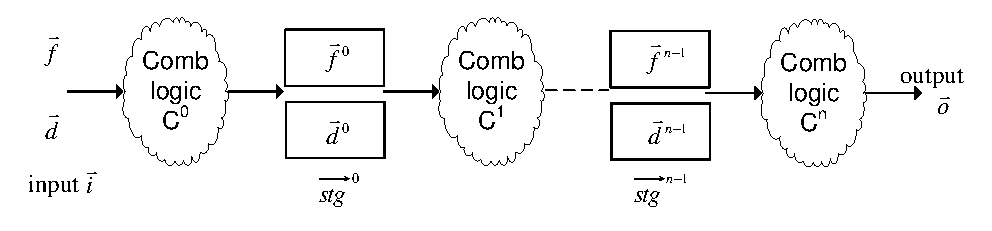
\includegraphics[width=\textwidth]{pipemod1}
\end{center}
\caption{包含流水线级和流控机制的一般性编码器模型}
  \label{fig_pipeenc}
\end{figure}



在本文中,
上标始终意味着流水线级,
而下标,,
如小节\ref{subsec_fsm}指出,
始终意味着在展开的迁移关系序列中的步。
例如,
$\vec{stg}^j$ 是第$j$个流水线级。
而$\vec{stg}^j_i$ 该第$j$流水线级
在第$i$步的取值。

\subsection{算法框架}

基于图\ref{fig_pipeenc}所示的编码器结构,
我们算法的框架为:

\begin{enumerate}
 \item 调用算法\ref{alg_fofc} 已将$\vec{i}$ 划分为$\vec{f}$ 和$\vec{d}$。
 \item 调用算法\ref{algo_infer} 以推导能够使得$\vec{d}$
 被唯一决定的$valid(\vec{f})$和其对应的$p$, $l$ 和$r$。
 \item 在小节\ref{sec_pipeinfer},
 找到每一个流水线级$\vec{stg}^j$中的$\vec{f}^j$ 和$\vec{d}^j$ 。
 \item 在小节\ref{sec_char},
 为每一个流水线级$\vec{stg}^j$
 和输入向量 $\vec{i}$特征化布尔函数。
\end{enumerate}



\section{推导流水线结构}\label{sec_pipeinfer}


\subsection{压缩$r$ 和$l$}\label{reduceing}

\begin{algorithm}[t]
\begin{algorithmic}[1]
\FOR{$r':=r \to 0$} 
\label{testr_1}
  \IF{$r'\equiv 0$ or $F_{PC}(p,l,r'-1)\wedge valid(\vec{f}_{p+l})$ 对于某些$i\in \vec{i}$可满足} 
    \STATE break
  \ENDIF
\ENDFOR
\RETURN $r'$
\caption{压缩$r$}
\label{algo_remove2}
\end{algorithmic}
\end{algorithm}

由于算法\ref{algo_infer} 同时增加$p$, $l$ 和$r$ ,
因此$l$ 和$r$存在一定程度的冗余。
因此我们需要首先在算法\ref{algo_remove2}中压缩$r$。


在行\ref{testr_1},
我们将推导的谓词$valid(\vec{f})$ 和$F_{PC}(p,l,r'-1)$与在一起。
当该公式可满足时,
则$r'$ 是最后一个使得$F_{PC}(p,l,r')\wedge valid(\vec{f}_{p+l})$ 不可满足的值,
我们将其直接直接返回。
另一方面,
当$r'\equiv 0$,
$F_{PC}(p,l,0)$ 肯定已经在上一个迭代中被测试,
且结果为不可满足。
此时我们直接返回$0$。


这样,
我们从算法\ref{algo_remove2}得到了一个压缩的$r$,
使得$\vec{i}_{p+l}$ 可以被$<\vec{o}_{p},\dots,\vec{o}_{p+l+r}>$唯一决定。

\begin{figure}[t]
\begin{center}
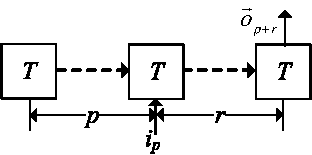
\includegraphics[width=0.5\textwidth]{pc1}
\end{center}
\caption{使用削减的输出序列恢复输入}
  \label{fig_pc1}
\end{figure}

我们进一步要求:
\begin{enumerate}
 \item 如图\ref{fig_pc1}所示,
 $l$ 可以被削减为0。
 这意味着$\vec{i}_{p}$ 可以被$<\vec{o}_{p},\dots,\vec{o}_{p+r}>$唯一决定。
 即所有的未来输出。
 \item 上述的输出序列$<\vec{o}_{p},\dots,\vec{o}_{p+r}>$
 能被进一步压缩为$\vec{o}_{p+r}$。
 这意味着只需$\vec{o}_{p+r}$ 即可唯一决定$\vec{i}_p$。
\end{enumerate}

检验这两个要求等价于
检查$F'_{PC}(p,r)\wedge valid(\vec{f}_{p+l})$的不可满足性
其中$F'_{PC}(p,r)$ 定义如下:

\begin{equation}\label{uniqt11}
% \begin{split}
F'_{PC}(p,r):=
\left\{
\begin{array}{cc}
&\bigwedge_{m=0}^{p+r}
\{
(\vec{s}_{m+1},\vec{o}_m)\equiv T(\vec{s}_m,\vec{i}_m)
\}
\\
\wedge&\bigwedge_{m=0}^{p+r}
\{
(\vec{s'}_{m+1},\vec{o'}_m)\equiv T(\vec{s'}_m,\vec{i'}_m)
\}
\\
\wedge&\vec{o}_{p+r}\equiv \vec{o'}_{p+r} \\
\wedge& i_{p}\equiv 1 \wedge  i'_{p}\equiv 0
% \wedge&\bigwedge_{m=0}^{p+l+r}assertion(\vec{i}_m) \\
% \wedge&\bigwedge_{m=0}^{p+l+r}assertion(\vec{i'}_m)
\end{array}
\right\}
% \end{split}
\end{equation}


该要求看起来远远强于(\ref{uniqt1})。
我们将在实验结果中指出他们总能够满足。



\subsection{推导流水线结构}\label{subsec_inferstage}

现在,
基于上述推导的$p$ 和$r$,
我们将公式(\ref{uniqt11}) 中的$F'_{PC}$推广到下面定义的更广泛的形式。
它能够检查任意变量$v$ 在步$j$
能否被向量$\vec{w}$ 在步$k$唯一决定。
现在$v$ 和$\vec{w}$ 可以使输入,输出或者状态向量。

\begin{equation}\label{uniqt2}
% \begin{split}
F''_{PC}(p,r,v,j,\vec{w},k):=
\left\{
\begin{array}{cc}
&\bigwedge_{m=0}^{p+r}
\{
(\vec{s}_{m+1},\vec{o}_m)\equiv T(\vec{s}_m,\vec{i}_m)
\}
\\
\wedge&\bigwedge_{m=0}^{p+r}
\{
(\vec{s'}_{m+1},\vec{o'}_m)\equiv T(\vec{s'}_m,\vec{i'}_m)
\}
\\
\wedge&\vec{w}_{k}\equiv \vec{w'}_{k} \\
\wedge& v_{j}\equiv 1 \wedge  v'_{j}\equiv 0
% \wedge&\bigwedge_{m=0}^{p+l+r}assertion(\vec{i}_m) \\
% \wedge&\bigwedge_{m=0}^{p+l+r}assertion(\vec{i'}_m)
\end{array}
\right\}
% \end{split}
\end{equation}

很明显,
当$F''_{PC}(p,r,v,j,\vec{w},k)$ 不可满足时,
$\vec{w}_k$ 能唯一决定$v_j$.

对于$0\le j\le n-1$,
在第$j$流水线级$\vec{stg}^j$,
其留空向量$\vec{f}^j$ 包含所有的
能够在第$j-((n-1)-(p+r))$-th 步被$\vec{o}$
在第$p+r$步唯一决定的状态变量$s\in \vec{s}$。
注意在这里不需要约束$valid(\vec{f}_p)$。
这可以形式化的定义为:

\begin{equation}\label{stgn_fj}
\vec{f}^{j} :=
 \left\{
 s\in \vec{s} ~|
\begin{array}{cc}
 F''_{PC}(p,r,s,j-D,\vec{o},p+r)\\
 ~is~unsatisfiable
\end{array}
\right\}
\end{equation}

其中:

\begin{equation}\label{stgn_def}
\begin{array}{ccc}
% S             & := & \vec{s}/\bigcup_{j<k\le n-2}\vec{stg}^{k}\\
D             & := & (n-1)-(p+r)\\
\end{array}
\end{equation}

而在第$j$流水线级$\vec{stg}^j$中的数据向量$\vec{d}^j$
包含能够在第$j-((n-1)-(p+r))$步被
$\vec{o}$ 在第$p+r$步唯一决定的所有$s\in \vec{s}$。
注意这里我们需要强制$valid(\vec{f}_p)$。
这可以被形式化的定义为:

\begin{equation}\label{stgn_dj}
\vec{d}^{j} :=
 \left\{
 s\in \vec{s} ~|
 \begin{array}{cc}
 F''_{PC}(p,r,s,j-D,\vec{o},p+r)\wedge valid(\vec{f}_p)\\
 ~is~unsatisfiable
 \end{array}
\right\}
\end{equation}


\section{特征化流水线级和输入的布尔函数}\label{sec_char}
\subsection{特征化最后一个流水线级的布尔函数}

从公式(\ref{stgn_fj})可知,
每个寄存器$s\in \vec{f}^{n-1}$ 能过被$\vec{o}$ 在第$p+r$步唯一决定。
也就是,
$F''_{PC}(p,r,s,p+r,\vec{o},p+r)$ 不可满足且可以划分为:

\begin{equation}
 \phi_A :=
 \left\{
\begin{array}{cc}
&\bigwedge_{m=0}^{p+r}
\{
(\vec{s}_{m+1},\vec{o}_m)\equiv T(\vec{s}_m,\vec{i}_m)
\}
\\
\wedge& s_{p+r}\equiv 1
\end{array}
\right\}
\end{equation}

\begin{equation}
% \begin{split}
\phi_B :=
\left\{
\begin{array}{cc}
&\bigwedge_{m=0}^{p+r}
\{
(\vec{s'}_{m+1},\vec{o'}_m)\equiv T(\vec{s'}_m,\vec{i'}_m)
\}
\\
\wedge&\vec{o}_{p+r}\equiv \vec{o'}_{p+r} \\
\wedge& s'_{p+r}\equiv 0
% \wedge&\bigwedge_{m=0}^{p+l+r}assertion(\vec{i}_m) \\
% \wedge&\bigwedge_{m=0}^{p+l+r}assertion(\vec{i'}_m)
\end{array}
\right\}
% \end{split}
\end{equation}

因为$F''_{PC}(p,r,s,p+r,\vec{o},p+r)$ 等价于$\phi_A \wedge \phi_B$,
所以$\phi_A \wedge \phi_B$ 不可满足
而$\phi_A$ 和$\phi_B$ 的共同变量集合是$\vec{o}_{p+r}$。

根据\cite{InterpBoolFunction},
$\phi_A$ 相对于$\phi_B$ 的Craig插值$\phi_I$可以被计算出来,
只引用$\vec{o}_{p+r}$,
并且覆盖所有能使$s_{p+r}\equiv 1$的$\vec{o}_{p+r}$ 。
同时,
$\phi_I\wedge \phi_B$ 不可满足
这意味着$\phi_I$ 并不覆盖任何使得$s_{p+r}\equiv 0$的$\vec{o}_{p+r}$ 。

因此,
$\phi_I$ 可以作为
从$\vec{o}$恢复$s\in \vec{f}^{n-1}$的布尔函数。

通过将$F''_{PC}(p,r,s,p+r,\vec{o},p+r)$ 替换为$F''_{PC}(p,r,s,p+r,\vec{o},p+r)\wedge valid(f_p)$,
我们可以类似的特征化恢复$s\in\vec{d}^{n-1}$的布尔函数。

\subsection{特征化恢复其他流水线级的布尔函数}
根据图\ref{fig_pipeenc},
% Similar to last subsection,
$\vec{f}^j$ 在第$j-D$步可以被$\vec{stg}^{j+1}$ 在第$j-D+1$步唯一决定。
因此我们将不可满足公式$F''_{PC}(p,r,s,j-D,\vec{stg}^{j+1},j-D+1)$
划分为下列两个公式:

\begin{equation}
 \phi_A :=
 \left\{
\begin{array}{cc}
&\bigwedge_{m=0}^{p+r}
\{
(\vec{s}_{m+1},\vec{o}_m)\equiv T(\vec{s}_m,\vec{i}_m)
\}
\\
\wedge& s_{j-D}\equiv 1
\end{array}
\right\}
\end{equation}

\begin{equation}
% \begin{split}
\phi_B :=
\left\{
\begin{array}{cc}
&\bigwedge_{m=0}^{p+r}
\{
(\vec{s'}_{m+1},\vec{o'}_m)\equiv T(\vec{s'}_m,\vec{i'}_m)
\}
\\
\wedge&\vec{stg}^{j+1}_{j-D+1}\equiv \vec{stg'}^{j+1}_{j-D+1} \\
\wedge& s'_{j-D}\equiv 0
% \wedge&\bigwedge_{m=0}^{p+l+r}assertion(\vec{i}_m) \\
% \wedge&\bigwedge_{m=0}^{p+l+r}assertion(\vec{i'}_m)
\end{array}
\right\}
% \end{split}
\end{equation}

再一次,
$\phi_A$ 相对于$\phi_B$ 的Craig插值$\phi_I$可以被构造出来,
并用做从$\vec{stg}^{j+1}$恢复$s\in\vec{f}^{j}$的布尔函数。

类似的,
将$F''_{PC}(p,r,s,j-D,\vec{stg}^{j+1},j-D+1)$  替换为
$F''_{PC}(p,r,s,j-D,\vec{stg}^{j+1},j-D+1)\wedge valid(f_p)$ ,
我们能特征化从$\vec{stg}^{j+1}$恢复$s\in\vec{d}^{j}$的布尔函数。

\subsection{特征化从第0级流水线恢复输入向量的布尔函数}

根据图\ref{fig_pipeenc},
$\vec{f}$ 在第$p$步能够被$\vec{stg}^0$ 在第$p$步唯一决定。
$F''_{PC}(p,r,i,p,\vec{stg}^0,p)$ 不可满足并可以划分为以下两个公式:

\begin{equation}
% \begin{split}
\phi_A:=
\left\{
\begin{array}{cc}
&\bigwedge_{m=0}^{p+r}
\{
(\vec{s}_{m+1},\vec{o}_m)\equiv T(\vec{s}_m,\vec{i}_m)
\}
\\
\wedge& i_{p}\equiv 1
% \wedge&\bigwedge_{m=0}^{p+l+r}assertion(\vec{i}_m) \\
% \wedge&\bigwedge_{m=0}^{p+l+r}assertion(\vec{i'}_m)
\end{array}
\right\}
% \end{split}
\end{equation}

\begin{equation}
% \begin{split}
\phi_B:=
\left\{
\begin{array}{cc}
&\bigwedge_{m=0}^{p+r}
\{
(\vec{s'}_{m+1},\vec{o'}_m)\equiv T(\vec{s'}_m,\vec{i'}_m)
\}
\\
\wedge&\vec{stg}^0_p\equiv \vec{stg'}^0_p \\
\wedge& i'_{p}\equiv 0
% \wedge&\bigwedge_{m=0}^{p+l+r}assertion(\vec{i}_m) \\
% \wedge&\bigwedge_{m=0}^{p+l+r}assertion(\vec{i'}_m)
\end{array}
\right\}
% \end{split}
\end{equation}

再一次,
$\phi_A$ 相对于$\phi_B$的Craig插值$\phi_I$
可以被用作从$\vec{stg}^0$恢复$i\in\vec{f}$的布尔函数。

类似的,
通过替换$F''_{PC}(p,r,i,p,\vec{stg}^0,p)$ 为$F''_{PC}(p,r,i,p,\vec{stg}^0,p)\wedge valid(\vec{f}_p)$,
我们可以特征化从$\vec{stg}^0$恢复$i\in\vec{d}$的布尔函数。



\section{实验结果}\label{sec_exp}
我们使用OCaml 语言实现了上述算法,
并使用MiniSat 1.14 \cite{EXTSAT}求解产生的CNF公式。
所有的实验使用一台包含16 个Intel Xeon E5648 2.67GHz处理器,
192GB 内存, 和CentOS 5.4 Linux操作系统的服务器上。

\subsection{比较时间和面积}
表\ref{tab_bench} 给出本文中使用的benchmark。
第2和3分别给出输入,输出和寄存器个数。
第4列给出了将编码器映射至LSI10K 库所得到的面积。
本文中,
所有的面积和延迟使用同样的设置得到。


\begin{table*}[t]
\caption{Benchmark和实验结果}
\begin{tabular}{|c|c|c|c|c|c|c|c|c|c|c|}
\hline
 Names     & \multicolumn{4}{|c|}{编码器}                                        &   \multicolumn{3}{|c|}{\cite{ShenTCAD11}产生}      &   \multicolumn{3}{|c|}{本文产生} \\
           & \multicolumn{4}{|c|}{}                                              &   \multicolumn{3}{|c|}{的解码器}                   &   \multicolumn{3}{|c|}{的解码器} \\\cline{2-11}
           &    \#   &   \#    &面积  & 解码器                                   &运行 &延迟 &面积                                    &运行 &延迟 &面积\\
           & in/out  &  reg    &      &   藐视                                   &时间 &(ns) &                                        &时间 &(ns) &    \\\hline\hline
 pcie      & 10/11   & 23      & 326  &PCIE 2.0 \cite{pcie21}                    &0.37 &7.20 &624                                     &8.08 & 5.89&652 \\\hline
 xgxs      & 10/10   & 16      & 453  &     以太网   clause 48 \cite{IEEE8023_S4}&0.21 &7.02 &540                                     &4.25 & 5.93&829 \\\hline
 t2eth     & 14/14   & 49      & 2252 &    以太网   clause 36 \cite{IEEE8023_S4} &12.7 &6.54 &434                                     &430.4& 6.12&877 \\\hline
scrambler  &64/64    & 58      & 1034 & inserting 01 flipping                    &     \multicolumn{6}{|c|}{no pipeline }\\\cline{1-5}
 xfi       & 72/66   & 72      & 7772 &     以太网   clause 49 \cite{IEEE8023_S4}&     \multicolumn{6}{|c|}{stages found}\\\hline
\end{tabular}\label{tab_bench}
\end{table*}





第6到8列分别给出了论文\cite{ShenTCAD11}的算法产生非流水解码器的运行时间,
以及该解码器的延迟和面积。
而第9到11列分别给出了本文算法的类似信息。

比较第7和10列可知
延迟得到了明显的改善。

一个比较令人惊讶的事实是,
两个最大的benchmarks scrambler 和xfi 并不包含流水线。
我们研究并确认了这一点。
他们的面积如此之大是因为使用了很宽的64到72 位数据路径。

\subsection{PCIE推导的流水线结构}

对于benchmark pcie,
存在两个流水线级,
其中包含的流控向量和数据向量如图\ref{tab_pcie}所示。

\begin{table}[t]
\centering
\caption{pcie推导的流水线结构}
\begin{tabular}{|c|c|c|c|}
\hline
                       & input                  & pipeline stage 0          &  pipeline stage 1    \\\hline\hline
流控                   &CNTL\_TXEnable\_P0      & InputDataEnable\_P0\_reg  & OutputData\_P0\_reg[9:0]\\
向量                   &                        &                           & OutputElecIdle\_P0\_reg \\\hline
流控                   &CNTL\_TXEnable\_P0      & InputDataEnable\_P0\_reg  & true \\
谓词                   &                        &                           &  \\\hline
数据                   &TXDATA[7:0]             & InputData\_P0\_reg[7:0]   & \\
向量                   &TXDATAK                 & InputDataK\_P0\_reg       & \\\hline
\end{tabular}\label{tab_pcie}
\end{table}


有一个有趣的事实是流水线级1的数据向量是空集。
而所有的流水线寄存器都被识别成为流控向量。
我们研究了源代码,
发现这些流水线寄存器全部都被直接送给输出向量。
因此他们很明显都能够被$\vec{o}$唯一决定。
伊霓裳这并不影响所产生的解码器的正确性。



\subsection{xgxs推导的流水线结构}


对于benchmark xgxs,
只有一级流水线,
其中的流控和数据向量如图\ref{tab_xgxs}所示。

\begin{table}[b]
\centering
\caption{xgxs推导的流水线结构}
\begin{tabular}{|c|c|c|}
\hline
                       & input                  &  pipeline stage 0    \\\hline\hline
流控向量               &bad\_code               & bad\_code\_reg\_reg\\\hline
流控谓词               &!bad\_code              & !bad\_code\_reg\_reg \\\hline
数据向量               &encode\_data\_in[7:0]   &ip\_data\_latch\_reg[2:0] \\
                       &konstant                &plus34\_latch\_reg     \\
                       &                        &data\_out\_latch\_reg[5:0]\\
                       &                        &konstant\_latch\_reg   \\
                       &                        &kx\_latch\_reg         \\
                       &                        &minus34b\_latch\_reg   \\\hline
\end{tabular}\label{tab_xgxs}
\end{table}


\subsection{t2ether推导的流水线结构}


\begin{table}[t]
\centering
\caption{t2ether推导的流水线结构}
\begin{tabular}{|c|c|c|c|c|c|}
\hline
                       & input                        & pipeline                  &  pipeline          &  pipeline       &  pipeline               \\
                       &                              & stage 0                   &  stage 1           &  stage 2        &  stage 3                \\\hline\hline
流控                   & tx\_enc\_ctrl\_sel[3:0]      &qout\_reg\_0\_8            & qout\_reg\_0\_9    &qout\_reg[9:0]\_2&qout\_reg[7:1]\_3        \\
向量                   &                              &qout\_reg\_2\_4            & qout\_reg\_1\_5    &                 &qout\_reg\_8\_1          \\
                       &                              &qout\_reg\_1\_4            & qout\_reg\_2\_5    &                 &qout\_reg\_9\_1          \\
                       &                              &                           & qout\_reg\_0\_10   &                 &qout\_reg\_3\_4          \\
                       &                              &                           &                    &                 &qout\_reg\_0\_4          \\
                       &                              &                           &                    &                 &qout\_reg\_3\_5          \\
                       &                              &                           &                    &                 &qout\_reg\_0\_7          \\
                       &                              &                           &                    &                 &sync1\_reg1              \\
                       &                              &                           &                    &                 &sync1\_reg               \\
                       &                              &                           &                    &                 &Q\_reg1                  \\
                       &                              &                           &                    &                 &Q\_reg                         \\\hline
数据                   &txd[7:0]                      &qout\_reg[7:0]             &qout\_reg[7:0]\_1   &                 &                         \\
向量                   &                              &                           &                    &                 &                         \\\hline
\end{tabular}\label{tab_t2ether}
\end{table}


对于benchmark t2ether,
有3级流水线,如图\ref{tab_t2ether}所示。
流控谓词比较复杂,
因此我们将他们单独列在下面而不是图\ref{tab_t2ether}中。
输入流控谓词$f$ 为:
\begin{multline}
\begin{array}{l}
( tx\_enc\_ctrl\_sel[2]~\&~tx\_enc\_ctrl\_sel[3] ) | \\
( tx\_enc\_ctrl\_sel[2]~\&~!tx\_enc\_ctrl\_sel[3]~\&~!tx\_enc\_ctrl\_sel[0]~\&~tx\_enc\_ctrl\_sel[1] ) | \\
( !tx\_enc\_ctrl\_sel[2]~\&~tx\_enc\_ctrl\_sel[3] ) | \\
( !tx\_enc\_ctrl\_sel[2]~\&~!tx\_enc\_ctrl\_sel[3]~\&~tx\_enc\_ctrl\_sel[0] )
\end{array}
\end{multline}

第零级流控谓词$valid(\vec{f}^0)$ :
\begin{multline}
\begin{array}{l}
( qout\_reg\_2\_4~\&~qout\_reg\_1\_4~\&~!qout\_reg\_0\_8) | \\
( !qout\_reg\_2\_4~\&~qout\_reg\_0\_8)
\end{array}
\end{multline}

第一级流控谓词$valid(\vec{f}^1)$ 为:

\begin{multline}
\begin{array}{l}
( qout\_reg\_2\_5~\&~qout\_reg\_1\_5~\&~qout\_reg\_0\_10~\&~!qout\_reg\_0\_9) | \\
( qout\_reg\_2\_5~\&~qout\_reg\_1\_5~\&~!qout\_reg\_0\_10) | \\
( qout\_reg\_2\_5~\&~!qout\_reg\_1\_5~\&~!qout\_reg\_0\_10) | \\
( !qout\_reg\_2\_5~\&~qout\_reg\_0\_10~\&~qout\_reg\_0\_9) | \\
( !qout\_reg\_2\_5~\&~!qout\_reg\_0\_10)
\end{array}
\end{multline}


最后两级的流控谓词$valid(\vec{f}^2)$ 和$valid(\vec{f}^3)$ 均为$true$。































\section{相关工作}\label{sec_relwork}

\subsection{对偶综合}\label{subsec_compsyn_relat}
第一个对偶综合算法由沈\cite{ShenICCAD09}提出。
他通过迭代的展开迁移函数来检查解码器的存在性,
并通过遍历所有的输出向量取值来特征化解码器的布尔函数。
其主要弱点在于该算法不停机,
而且特征化解码器函数时速度太慢。

沈et al.\cite{ShenTCAD11} 和Liu et al.\cite{LiuICCAD11} 通过在状态序列上搜索环来解决停机问题。
而\cite{ShenTCAD12,LiuICCAD11} 通过Craig插值\cite{interp_McMillan}高效的特征化解码器函数。

沈et al.\cite{ShenTCAD12} 自动推导使得解码器存在的配置断言。

秦et al. \cite{QinTODAES15}
提出了第一个能处理流控机制的对偶综合算法。

Tu 和Jiang \cite{TuDAC13} 提出了一个突破性的算法以在恢复编码器输入时考虑其非限界的历史。


\subsection{程序取反}\label{subsec_proinv}
根据Gulwani \cite{dim_syn},
程序取反意味着为
特定程序$P$
生成一个具有反功能的程序$P^{-1}$。
因此,
程序取反非常类似于我们的对偶综合。

最早的程序取反算法基于proof的算法\cite{prog_inv},
只能处理非常小的程序和非常简单的语法。

Gl\"{u}ck et al. \cite{mtd_autoProginv} 取反一阶函数语言的程序,
通过基于LR的算法来去除非确定性。.
然而使用函数语言使得其应用场景和我们有很大的差别。

{Srivastava et al. \cite{prog_inv_rev,program_inversion_11} 假设反程序和原始程序的结构是类似的,
因此可能的反程序结构可以通过挖掘原始程序中的谓词,表达式和控制流得到。
这和本文发掘流水线级和流控机制类似。
该算法迭代的去掉不满足要求的解空间直至剩下正确的解。


\section{结论}\label{sec_conclude}
本文提出了第一个能同时处理流控机制和流水线的对偶综合算法。
实验结果表明本文算法总能够正确的产生带有流控机制和流水线的解码器。


% !Mode:: "Tex:UTF-8"
\chapter{面向流水线的对偶综合}
\label{chap:5}

\section{引言}
在通讯和多媒体芯片设计项目中,
最困难的一个工作是针对特定的协议,
如以太网\cite{IEEE8023_S4} 和PCI Express \cite{pcie21},
设计相应的编码器和解码器.
其中编码器负责将输入$\vec{i}$ 映射至输出$\vec{o}$,
而解码器则负责从$\vec{o}$中恢复$\vec{i}$。
对偶综合\cite{ShenICCAD09,ShenTCAD11,ShenTCAD12,LiuICCAD11,LiuTCAD12,TuDAC13}
假设$\vec{i}$ 总能够被$\vec{o}$的一个有限序列唯一决定,
以自动产生相应的解码器。
其中,
解码器的布尔函数可以使用Jiang et al. \cite{InterpBoolFunction}提出的算法,
该算法基于Craig插值\cite{Craig}。

通过研究现有的工业界编码器,我们发现他们都含有流水线结构以提高运行频率。
\begin{figure}[t]
\begin{center}
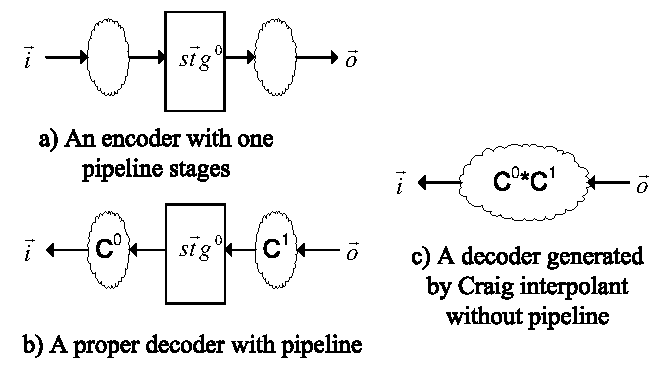
\includegraphics[width=\textwidth]{pipeline_pipeline}
\end{center}
\caption{带有流水线的编码器和解码器}
  \label{fig_pipe}
\end{figure}

一个带有流水线的简单编码器如图\ref{fig_pipe}a)所示。
他的关键数据路径被第一级流水线切割成为两段,
从而使得运行频率得到两倍的提升。

他的第一级流水线$\vec{stg}^0$ 包含数个寄存器。
其中输入变量$\vec{i}$ 被用于计算该级流水线$\vec{stg}^0$,
而流水线$\vec{stg}^0$ 则被用于计算$\vec{o}$。
根据该结构,
$\vec{stg}^0$ 能够被$\vec{o}$唯一决定,
而$\vec{i}$ 能够被$\vec{stg}^0$唯一决定。

因此,
一个由人类程序员设计的合理解码器,
应当如图\ref{fig_pipe}b)所示,
从$\vec{o}$ 中使用组合逻辑$C^1$恢复$\vec{stg}^0$ ,
并进一步使用组合逻辑$C^0$从$\vec{stg}^0$ 中恢复$\vec{i}$ 。
在此类解码器中,
关键路径被流水线级$\vec{stg}^0$切断,
以改善时序。



然而,
目前所有的对偶综合算法\cite{ShenTCAD11,ShenTCAD12,LiuICCAD11,LiuTCAD12,TuDAC13}
均使用Jiang提出的基于\cite{Craig}的算法 \cite{InterpBoolFunction}。
如图\ref{fig_pipe}c)所示,
这些算法从$\vec{o}$中使用一个大型组合逻辑$C^0*C^1$直接恢复$\vec{i}$,
这使得他们变得不必要的很慢,因为没有流水线寄存器切断这段复杂逻辑。

为了产生如图\ref{fig_pipe}b) 所示的解码器,
本文提出了一个新颖的算法。首先找到编码器中每一个流水线级$\vec{stg}^j$中的寄存器,
然后特征化每一个流水线级$\vec{stg}^j$的布尔函数,
已从下一个流水线级$\vec{stg}^{j+1}$ 或输出$\vec{o}$之中恢复$\vec{stg}^j$。
最终特征化$\vec{i}$的布尔函数以葱
第一个流水线级$\vec{stg}^0$中恢复$\vec{i}$。

%\begin{figure}[t]
%\begin{center}
%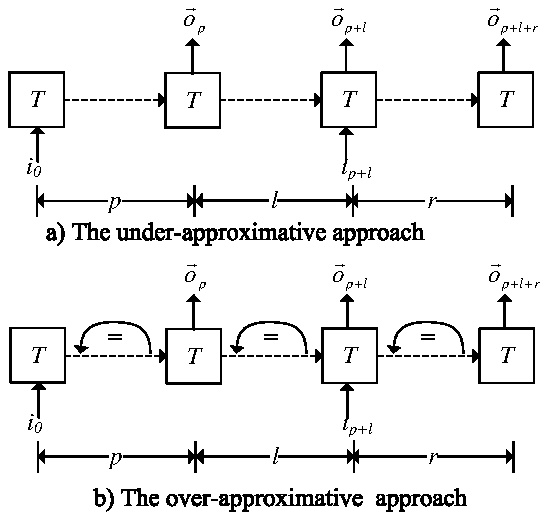
\includegraphics[width=\textwidth]{pcln_pipeline}
%\end{center}
%\caption{下估计和上估计算法}
%  \label{fig_pc}
%\end{figure}

在复杂的工业界实际编码器,
如PCI Express \cite{pcie21} 和以太网\cite{IEEE8023_S4},
上的实验表明,
该算法总能够产生带有流水线级的快速解码器。.


\emph{本文剩余的内容安排如下}.
%Section \ref{sec_casestudy} explains our ideas with a simple example.
%第\ref{sec_prem} 节介绍了背景知识;
第\ref{sec_pipeinfer_chap4} 节推导流水线结构,
而第\ref{sec_char_chap4} 节特征化每一个流水线级和输入的布尔函数;
第\ref{sec_exp_chap4} 和\ref{sec_conclude_chap4} 节给出实验结果和结论。


%
%
%\section{背景知识}\label{sec_prem}
%
%% \subsection{Flow control mechanism}\label{subsec_fc}
%
%
%
%\subsection{命题逻辑可满足}\label{subsec_SAT}
%布尔集合为$\mathbb{B}=\{0,1\}$。
%变量向量表示为$\vec{v}=(v,\dots)$。
%向量$\vec{v}$ 中的变量个数表示为$|\vec{v}|$。
%若一个变量$v$ 是$\vec{v}$的成员,
%则记为$v\in\vec{v}$;
%否则$v\notin\vec{v}$.
%$v\cup\vec{v}$ 是包含$v$ 和$\vec{v}$的所有成员的新向量。
%$\vec{v}/\vec{w}$ 是一个包含$\vec{v}$ 的所有成员但是不包含$\vec{w}$的任意成员的新向量。
%$\vec{a}\cup\vec{b}$ 是包含$\vec{a}$ 和$\vec{b}$的所有成员的新向量。
%$\vec{v}$ 的赋值集合记为$[\![\vec{v}]\!]$,
%比如,
%$[\![(v_1,v_2)]\!]=\{(0,0),(0,1),(1,0),(1,1)\}$。
%
%
%对于变量集合$V$上的公式$F$,
%起命题逻辑可满足(SAT)  问题是指
%如何找到$V$的一个赋值函数$A:V\to \mathbb{B}$,
%使得$F$ 能够被赋值为$1$。
%若$A$ 存在,则$F$ 是可满足的;
%否则,
%是不可满足的。
%
%对于公式$\phi_A$ 和$\phi_B$,
%若$\phi_A\wedge \phi_B$ 不可满足,
%则存在公式$\phi_I$ 仅包含$\phi_A$ 和$\phi_B$ 的共同变量,
%并使得$\phi_A\Rightarrow \phi_I$
%且$\phi_I\wedge \phi_B$ 不可满足。
%$\phi_I$ 称为$\phi_A$ 相对于$\phi_B$的Craig插值\cite{Craig}。
%$\phi_I$ 可以使用McMillan提出的算法\cite{interp_McMillan}进行计算,
%并应用于从一个布尔关系特征化出一个布尔函数\cite{InterpBoolFunction}。
%
%
%
%\subsection{游有限状态机}\label{subsec_fsm}
%
%
%编码器使用有限状态机模型(FSM) $M=(\vec{s},\vec{i},\vec{o},T)$,
%其中$\vec{s}$为状态变量向量,
%$\vec{i}$为输入变量向量,
%$\vec{o}$为输出变量向量,
%$T: [\![\vec{s}]\!]\times [\![\vec{i}]\!]\to [\![\vec{s}]\!]\times [\![\vec{o}]\!]$
%是一个状态迁移函数,
%用于从当前状态和输入变量向量,
%计算出下一状态和输出变量向量。
%
%$M$的行为可以通过展开迁移关系进行推导。
%在第$n$步的$s\in\vec{s}$,$i\in\vec{i}$ 和$o\in\vec{o}$
%分别表示为$s_n$, $i_n$ 和$o_n$。
%另外,
%在第$n$步的单个状态,输入和输出变量分别表示为$\vec{s}_n$,$\vec{i}_n$ 和$\vec{o}_n$。
%一个路径是指$<\vec{s}_n,\dots,\vec{s}_m>$,
%其中对于$n\le j< m$,
%有$\exists \vec{i}_j\vec{o}_j (\vec{s}_{j+1},\vec{o}_j)\equiv T(\vec{s}_j,\vec{i}_j)$ 。
%一个环是一个路径$<\vec{s}_n,\dots,\vec{s}_m>$ 满足$\vec{s}_n\equiv \vec{s}_m$。
%
%\subsection{用于确定一个输入变量能否被输出向量的有限序列唯一决定的停机算法}\label{subsec_chkextdec}
%
%该算法\cite{ShenTCAD11} 迭代的展开迁移函数。
%对于每次迭代,
%其分别调用一个下估计和一个上估计算法已给出确定的答案。
%这两个算法分别在\ref{subsub_sound} 和\ref{subsub_complete}中给出。
%我们酱紫啊\ref{subsub_algo} 中指出
%这两者将最终收敛。
%
%\subsubsection{下估计算法}\label{subsub_sound}
%
%如图\ref{fig_pc}a)所示,
%在展开的迁移函数序列上,
%输入变量$i\in\vec{i}$ 能够被唯一决定的充分条件是,
%存在$p$,$l$ 和$r$,
%使得对于输出向量序列$<\vec{o}_p,\dots,\vec{o}_{p+l+r}>$的任意值,
%$i_{p+l}$不能同时为0和1。
%折等价于公式(\ref{uniqt1})中定义的$F_{PC}(p,l,r)$ 的不可满足性。
%
%\begin{multline}\label{uniqt1}
%% \begin{split}
%F_{PC}(p,l,r):=\\
%\left\{
%\begin{array}{cc}
%&\bigwedge_{m=0}^{p+l+r}
%\{
%(\vec{s}_{m+1},\vec{o}_m)\equiv T(\vec{s}_m,\vec{i}_m)
%\}
%\\
%\wedge&\bigwedge_{m=0}^{p+l+r}
%\{
%(\vec{s'}_{m+1},\vec{o'}_m)\equiv T(\vec{s'}_m,\vec{i'}_m)
%\}
%\\
%\wedge&\bigwedge_{m=p}^{p+l+r}\vec{o}_m\equiv \vec{o'}_m \\
%\wedge& i_{p+l}\equiv 1 \wedge  i'_{p+l}\equiv 0
%% \wedge&\bigwedge_{m=0}^{p+l+r}assertion(\vec{i}_m) \\
%% \wedge&\bigwedge_{m=0}^{p+l+r}assertion(\vec{i'}_m)
%\end{array}
%\right\}
%% \end{split}
%\end{multline}
%
%
%
%其中,
%$p$ 是前置状态序列的长度,
%$l$ 和$r$是两个用于唯一决定输入$i_{p+l}$的输出变量序列
%$<\vec{o}_{p+1},\dots,\vec{o}_{p+l}>$ 和$<\vec{o}_{p+l+1},\dots,\vec{o}_{p+l+r}>$
%的长度。
%行2对应于图\ref{fig_pc}a)中的路径,
%行3 是他的一个拷贝。
%他们的长度是一样的。
%行4 强制两者的输出序列具有相同的赋值,
%而行5 强制他们的输入$i_{p+l}$ 不同。
%
%根据公式(\ref{uniqt1}),
%对于 $p'\ge p$, $l'\ge l$ 和$r'\ge r$,
%$F_{PC}(p',l',r')$ 的短句集合是$F_{PC}(p,l,r)$的超集。
%因此,
%$F_{PC}(p,l,r)$的不可满足性
%可以扩展到任意更大的$p'\ge p$, $l'\ge l$ 和$r'\ge r$。
%
%
%\begin{proposition}\label{prop_pc1}
%若$F_{PC}(p,l,r)$ 不可满足,
%则对任意更大的$p$, $l$ 和$r$,
%$i_{p+l}$ 可以被$<\vec{o}_{p},\dots,\vec{o}_{p+l+r}>$ 唯一决定。
%\end{proposition}
%
%
%\subsubsection{上估计算法}\label{subsub_complete}
%
%若上一节定义的$F_{PC}(p,l,r)$ 可满足,
%则存在两种可能性:
%\begin{enumerate}
% \item
%$i_{p+l}$ 可以在更大的$p$, $l$ 和$r$时,
%被$<\vec{o}_{p},\dots,\vec{o}_{p+l+r}>$ 唯一决定;
% \item
%$i_{p+l}$ 不能被任何$p$, $l$ 和$r$情况下的$<\vec{o}_{p},\dots,\vec{o}_{p+l+r}>$ 唯一决定。
%\end{enumerate}
%
%如果是第一种情况,
%则通过迭代的增大$p$, $l$ 和$r$,
%$F_{PC}(p,l,r)$ 总能够变成不可满足。
%而如果是第二种情况,
%则该算法不停机。
%
%
%
%\begin{algorithm}[t]
%\begin{algorithmic}[1]
%\STATE{输入 :输入变量$i\in\vec{i}$.}
%\STATE{输出: $i\in\vec{i}$ 是否能够被$\vec{o}$唯一决定,$p$, $l$ 和$r$的取值}
%\STATE $p$:= 0; ~$l$:= 0;~$r$:= 0\;
%\WHILE {$1$}
%\STATE   $p$++;~$l$++;~$r$++\;\label{linepc1}
%   \IF{$F_{PC}(p,l,r)$ 不可满足}
%    \RETURN (yes, $p$, $l$, $r$);
%   \label{lnsat}\ELSIF{$F_{LN}(p,l,r)$ 可满足}
%    \RETURN (no, $p$, $l$, $r$);
%   \ENDIF
%\ENDWHILE
%\caption{$CheckUniqueness(i)$: 检查
%$i\in\vec{i}$ 能否被$\vec{o}$唯一决定的停机算法}
%\label{alg_pcln}
%\end{algorithmic}
%\end{algorithm}
%
%
%
%因此,
%为了得到停机算法
%我们需要区分上述两种情形。
%该方法如图\ref{fig_pc}b)所示,
%该图类似于图\ref{fig_pc}a),
%不过增加了三个新的约束用于检测在$<\vec{s}_{0},\dots,\vec{s}_{p}>$,$<\vec{s}_{p+1},\dots,\vec{s}_{p+l}>$ 和
%$<\vec{s}_{p+l+1},\dots,\vec{s}_{p+l+r}>$上的环。
%其形式化的定义如公式(\ref{uniqln})
%其中最后三行对应于新增加的三个环检测约束。
%
%\begin{multline}\label{uniqln}
%% \begin{split}
%F_{LN}(p,l,r):=\\
%\left\{
%\begin{array}{cc}
%&F_{PC}(p,l,r)\\
%\wedge&\bigvee_{x=0}^{p-1}\bigvee_{y=x+1}^{p} \{\vec{s}_x\equiv \vec{s}_y\wedge \vec{s'}_x\equiv \vec{s'}_y\} \\
%\wedge&\bigvee_{x=p+1}^{p+l-1}\bigvee_{y=x+1}^{p+l} \{\vec{s}_x\equiv \vec{s}_y\wedge \vec{s'}_x\equiv \vec{s'}_y\} \\
%\wedge&\bigvee_{x=p+l+1}^{p+l+r-1}\bigvee_{y=x+1}^{p+l+r} \{\vec{s}_x\equiv \vec{s}_y\wedge \vec{s'}_x\equiv \vec{s'}_y\}
%\end{array}
%\right\}
%% \end{split}
%\end{multline}
%
%
%
%当$F_{LN}(p,l,r)$ 可满足时,
%则$i_{p+l}$ 不能被$<\vec{o}_{p},\dots,\vec{o}_{p+l+r}>$唯一决定。
%更重要的是,
%通过展开这三个环
%我们可以把$F_{LN}(p,l,r)$ 的可满足性推广到更大的$p$, $l$ 和$r$上。
%这意味着:
%
%
%\begin{proposition}\label{prop_ln1}
%如果$F_{LN}(p,l,r)$ 可满足,
%则$i_{p+l}$ 对于任意更大的$p$, $l$ 和$r$,
%不能被$<\vec{o}_{p},\dots,\vec{o}_{p+l+r}>$ 唯一决定。
%\end{proposition}
%
%其正确性证明的细节见\cite{ShenTCAD11}。
%
%\subsubsection{完全算法}\label{subsub_algo}
%
%基于Propositions \ref{prop_pc1} 和\ref{prop_ln1},
%我们有如下算法\ref{alg_pcln}。
%该算法搜索$p$, $l$ 和$r$ 使得
%输入变量$i_{p+l}$ 能够被$<\vec{o}_{p},\dots,\vec{o}_{p+l+r}>$唯一决定。
%\begin{enumerate}
% \item
%一方面,
%如果存在这样的$p$, $l$ 和$r$,
%则令$p':=max(p,l,r)$, $l':=max(p,l,r)$ 和$r':=max(p,l,r)$。
%从Propositions \ref{prop_pc1},
%我们知道$F_{PC}(p',l',r')$ 不可满足。
%因此$F_{PC}(p,l,r)$ 总能在行\ref{linepc1}称为不可满足;
% \item
%另一方面,
%如果不存在$p$, $l$ 和$r$,
%则$p$, $l$ 和$r$ 总会变得比最长的无环路径更长,
%这意味着在$<\vec{s}_{0},\dots,\vec{s}_{p}>$,$<\vec{s}_{p+1},\dots,\vec{s}_{p+l}>$ 和
%$<\vec{s}_{p+l+1},\dots,\vec{s}_{p+l+r}>$上存在环。
%这将使得$F_{LN}(p,l,r)$ 在行\ref{lnsat}变得可满足。
%\end{enumerate}
%
%两种情况都将导致上述算法停机。
%其正确性和停机性证明的细节见\cite{ShenTCAD11} 。
%


\section{推导编码器的流水线结构}\label{sec_pipeinfer_chap4}

\subsection{流水线的一般性模型}
如图\ref{fig_pipeenc_chap4}所示,
我们假设
编码器有$n$ 级流水线。
如果我们把组合逻辑$C^j$ 视为一个函数,
则编码器可以用下列的公式表示:

\begin{equation}\label{equ_genpipe}
\begin{array}{cccc}
\vec{stg}^0   & := & C^0(\vec{i})         &\\
\vec{stg}^j   & := & C^j(\vec{stg}^{j-1}) & 1\le j\le n-1\\
\vec{o}       & := & C^n(\vec{stg}^{n-1}) &
\end{array}
\end{equation}


\begin{figure}[b]
\begin{center}
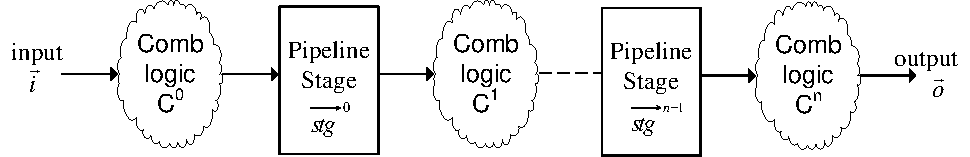
\includegraphics[width=\textwidth]{pipemod_pipeline}
\end{center}
\caption{编码器的一般性结构}
  \label{fig_pipeenc_chap4}
\end{figure}


因此,
每个$C^j$ 可以视为一个小型的编码器用于从$\vec{stg}^{j-1}$或$\vec{i}$中计算$\vec{stg}^j$ 或$\vec{o}$。


在本文的剩余部分,
上标始终表示特定的流水线级,
而下标则如小节\ref{subsec_fsm}所述,
表示在展开的迁移关系序列中的步数。
例如,
$\vec{stg}^j$ 是第$j$个流水线级。
而$\vec{stg}^j_i$ 则是该第$j$流水线级
在展开的迁移函数序列中的第$i$步的值。

\subsection{推导$p$, $l$ 和$r$}\label{subsec_inferplr}
在推导之前,
我们首先使用算法\ref{alg_pcln_chap1} 以得到$p$, $l$ 和$r$ 。

因为存在多于一个$i\in \vec{i}$,
我们需要为每一个$i\in \vec{i}$使用算法\ref{alg_pcln_chap1}
以得到他们对用的$p$, $l$ 和$r$ 。

然后我们将最终的$p$,$l$ 和$r$ 设置为所有$i\in \vec{i}$中最大的$p$, $l$ 和$r$ 。
根据公式\ref{uniqt1},
这些$p$, $l$ 和$r$ 能够使得$<o_{p},\dots,o_{p+l+r}>$ 唯一决定所有$i_{p+l}\in \vec{i}_{p+l}$。


\subsection{压缩$r$ 和$l$}\label{reduceing}

\begin{algorithm}[t]
\begin{algorithmic}[1]
\FOR{$r':=r \to 0$}
\label{testr_1}
  \IF{$r'\equiv 0$ or $F_{PC}(p,l,r'-1)$ 对于某些$i\in \vec{i}$是可满足的}
  \STATE  break;
  \ENDIF
\ENDFOR
\RETURN $r'$;
\caption{$RemoveRedundancy(p,l,r)$}
\label{algo_remove2_chap4}
\end{algorithmic}
\end{algorithm}



算法\ref{alg_pcln_chap1} 同步增长$p$, $l$ 和$r$ ,
因此在$l$ 和$r$中可能存在冗余。
因此我们需要首先在算法\ref{algo_remove2_chap4}中压缩$r$。


在行\ref{testr_1},
当$F_{PC}(p,l,r'-1)$ 可满足时,
则$r'$ 是最有一个使得$F_{PC}(p,l,r')$ 不可满足的,
我们将其直接返回。
另一方面,
当$r'\equiv 0$,
$F_{PC}(p,l,0)$ 已经在上一次迭代中被测试过,
且结果必然是不可满足。
在这种情况下我们返回$0$。


如此,
我们从算法\ref{algo_remove2_chap4}获得了一个压缩后的$r$ ,
它能使$\vec{i}_{p+l}$ 被$<\vec{o}_{p},\dots,\vec{o}_{p+l+r}>$唯一决定。

我们进一步要求:
\begin{enumerate}
 \item 如图\ref{fig_pc1_chap4}所示,
 $l$ 可以被压缩为0,
 这意味着$\vec{i}_{p}$ 能够被$<\vec{o}_{p},\dots,\vec{o}_{p+r}>$唯一决定,
 也就是说,
 所有的将来输出。
 \item 上述的序列$<\vec{o}_{p},\dots,\vec{o}_{p+r}>$
 可以被进一步压缩为$\vec{o}_{p+r}$.
 这意味着$\vec{o}_{p+r}$ 是在恢复$\vec{i}_p$时唯一被需要的输出。
\end{enumerate}

检查上述两个要求等价于下式的不可满足:

\begin{equation}\label{uniqt11_chap4}
% \begin{split}
F'_{PC}(p,r):=
\left\{
\begin{array}{cc}
&\bigwedge_{m=0}^{p+r}
\{
(\vec{s}_{m+1},\vec{o}_m)\equiv T(\vec{s}_m,\vec{i}_m)
\}
\\
\wedge&\bigwedge_{m=0}^{p+r}
\{
(\vec{s'}_{m+1},\vec{o'}_m)\equiv T(\vec{s'}_m,\vec{i'}_m)
\}
\\
\wedge&\vec{o}_{p+r}\equiv \vec{o'}_{p+r} \\
\wedge& i_{p}\equiv 1 \wedge  i'_{p}\equiv 0
% \wedge&\bigwedge_{m=0}^{p+l+r}assertion(\vec{i}_m) \\
% \wedge&\bigwedge_{m=0}^{p+l+r}assertion(\vec{i'}_m)
\end{array}
\right\}
% \end{split}
\end{equation}


该等式看起来似乎远强于等式(\ref{uniqt1})。
我们将在实验结果中指出,
该等式总能称为不满足。

\begin{figure}[b]
\begin{center}
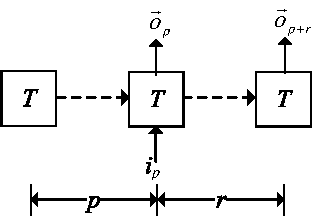
\includegraphics[width=0.4\textwidth]{pc1_pipeline}
\end{center}
\caption{从压缩的输出序列中恢复输入}
  \label{fig_pc1_chap4}
\end{figure}

\subsection{推导流水线}\label{subsec_inferstage}

基于上述的$p$ 和$r$,
我们将上述公式(\ref{uniqt11_chap4})中的$F'_{PC}$ 推广到下述公式
以便能够检查 $v$在第$j$步
是否能够被$\vec{w}$ 在第$k$步唯一决定。
现在$v$ 和$\vec{w}$ 可以使输入,输出和状态变量向量。

\begin{equation}\label{uniqt2}
% \begin{split}
F''_{PC}(p,r,v,j,\vec{w},k):=
\left\{
\begin{array}{cc}
&\bigwedge_{m=0}^{p+r}
\{
(\vec{s}_{m+1},\vec{o}_m)\equiv T(\vec{s}_m,\vec{i}_m)
\}
\\
\wedge&\bigwedge_{m=0}^{p+r}
\{
(\vec{s'}_{m+1},\vec{o'}_m)\equiv T(\vec{s'}_m,\vec{i'}_m)
\}
\\
\wedge&\vec{w}_{k}\equiv \vec{w'}_{k} \\
\wedge& v_{j}\equiv 1 \wedge  v'_{j}\equiv 0
% \wedge&\bigwedge_{m=0}^{p+l+r}assertion(\vec{i}_m) \\
% \wedge&\bigwedge_{m=0}^{p+l+r}assertion(\vec{i'}_m)
\end{array}
\right\}
% \end{split}
\end{equation}

很显然,
当$F''_{PC}(p,r,v,j,\vec{w},k)$ 不可满足时,
$\vec{w}_k$ 能够唯一决定$v_j$.

最后一集流水线$\vec{stg}^{n-1}$ 就是
所有能够被
在第$p+r$步的$\vec{o}$唯一决定的$s\in \vec{s}$。
其定义为:

\begin{equation}\label{stgn_1}
 \vec{stg}^{n-1} :=
\left\{
 s\in \vec{s} ~|
\begin{array}{cc}
 F''_{PC}(p,r,
 s,p+r,
 \vec{o},p+r)\\
 ~is~unsatisfiable
\end{array}
\right\}
\end{equation}


类似的,
对于$0\le j\le n-2$,
$\vec{stg}^j$ 在第$j-((n-2)-(p+r-1))$步
可以被$\vec{stg}^{j+1}$ 在第$j-((n-2)-(p+r-1))+1$步唯一决定。
我们可以定义$\vec{stg}^j$ 为:

\begin{equation}\label{stgn_def_chap4}
\begin{array}{ccc}
S             & := & \vec{s}/\bigcup_{j<k\le n-2}\vec{stg}^{k}\\
D             & := & (n-2)-(p+r-1)\\
\end{array}
\end{equation}

\begin{equation}\label{stgn_j}
\vec{stg}^{j} :=
 \left\{
 s\in S ~|
\begin{array}{cc}
 F''_{PC}(p,r,s,j-D,\vec{stg}^{j+1},j-D+1)\\
不可满足
\end{array}
\right\}
\end{equation}

基于等式(\ref{stgn_1}) 和(\ref{stgn_j}),
所有的流水线几都能够被推导出来。

\subsection{推导唯一决定输入的流水线级}\label{subsec_inferinput}

根据图\ref{fig_pipeenc_chap4},
 定义于(\ref{stgn_j}) 的$\vec{stg}^0$是唯一决定$\vec{i}$的流水线级。

然而在实际的解码器中,
并不一定是这种情形。
因此我们需要从$0$ 到$n-1$,
搜索最小的$j$ 使得
$\vec{i}$ 能够被$\vec{stg}^j$唯一决定。
即,
最小的能够使得$F''_{PC}(p,r,i,p,\vec{stg}^{j},j-D)$ 对所有$i\in \vec{i}$不可满足的$j$。
其中$D$ 定义于等式(\ref{stgn_def_chap4})。

\section{特征化输入向量和流水线级的布尔函数}\label{sec_char_chap4}
\subsection{特征化最后一个流水线级的布尔函数}

根据等式(\ref{stgn_1}),
每个寄存器$s\in \vec{stg}^{n-1}$ 都能够被$\vec{o}$ 在第$p+r$步唯一决定。
即,
$F''_{PC}(p,r,s,p+r,\vec{o},p+r)$ 不可满足,且可以被划分为:

\begin{equation}
 \phi_A :=
 \left\{
\begin{array}{cc}
&\bigwedge_{m=0}^{p+r}
\{
(\vec{s}_{m+1},\vec{o}_m)\equiv T(\vec{s}_m,\vec{i}_m)
\}
\\
\wedge& s_{p+r}\equiv 1
\end{array}
\right\}
\end{equation}

\begin{equation}
% \begin{split}
\phi_B :=
\left\{
\begin{array}{cc}
&\bigwedge_{m=0}^{p+r}
\{
(\vec{s'}_{m+1},\vec{o'}_m)\equiv T(\vec{s'}_m,\vec{i'}_m)
\}
\\
\wedge&\vec{o}_{p+r}\equiv \vec{o'}_{p+r} \\
\wedge& s'_{p+r}\equiv 0
% \wedge&\bigwedge_{m=0}^{p+l+r}assertion(\vec{i}_m) \\
% \wedge&\bigwedge_{m=0}^{p+l+r}assertion(\vec{i'}_m)
\end{array}
\right\}
% \end{split}
\end{equation}

由于$F''_{PC}(p,r,s,p+r,\vec{o},p+r)$ 等价于$\phi_A \wedge \phi_B$,
因此$\phi_A \wedge \phi_B$ 也是不可满足的。
而$\phi_A$ 和$\phi_B$ 的共同变量集合是$\vec{o}_{p+r}$。

根据文献\upcite{InterpBoolFunction},
$\phi_A$ 相对于$\phi_B$的Craig插值$\phi_I$  可以构造出来,
其中仅包含$\vec{o}_{p+r}$,
并覆盖所有使$s_{p+r}\equiv 1$得$\vec{o}_{p+r}$ 的赋值。
同时,
$\phi_I\wedge \phi_B$  不可满足,
这意味着$\phi_I$ 不能使$s_{p+r}\equiv 0$。

因此,
$\phi_I$ 能作为解码器的布尔函数以从$\vec{o}$中恢复$s\in \vec{stg}^{n-1}$ 。

\subsection{特征化其他流水线级的布尔函数}
类似于上一小节,
我们可以将公式(\ref{stgn_j})中的不可满足公式$F''_{PC}(p,r,s,j-D,\vec{stg}^{j+1},j-D+1)$
划分如下:

\begin{equation}
 \phi_A :=
 \left\{
\begin{array}{cc}
&\bigwedge_{m=0}^{p+r}
\{
(\vec{s}_{m+1},\vec{o}_m)\equiv T(\vec{s}_m,\vec{i}_m)
\}
\\
\wedge& s_{j-D}\equiv 1
\end{array}
\right\}
\end{equation}

\begin{equation}
% \begin{split}
\phi_B :=
\left\{
\begin{array}{cc}
&\bigwedge_{m=0}^{p+r}
\{
(\vec{s'}_{m+1},\vec{o'}_m)\equiv T(\vec{s'}_m,\vec{i'}_m)
\}
\\
\wedge&\vec{stg}^{j+1}_{j-D+1}\equiv \vec{stg'}^{j+1}_{j-D+1} \\
\wedge& s'_{j-D}\equiv 0
% \wedge&\bigwedge_{m=0}^{p+l+r}assertion(\vec{i}_m) \\
% \wedge&\bigwedge_{m=0}^{p+l+r}assertion(\vec{i'}_m)
\end{array}
\right\}
% \end{split}
\end{equation}

$\phi_A$ 相对于$\phi_B$的Craig 插值$\phi_I$  能够被构造出来,
并作为从$\vec{stg}^{j+1}$恢复$s\in \vec{stg}^{j}$的布尔函数。

\subsection{特征化输入变量的布尔函数}

根据小节\ref{sec_pipeinfer_chap4},
我们找到了使得$F''_{PC}(p,r,i,p,\vec{stg}^{j},j-D)$ 对所有$i\in \vec{i}$都不满足的$j$,
其中$D$ 在的公式(\ref{stgn_def_chap4})中定义。
$F''_{PC}(p,r,i,p,\vec{stg}^{j},j-D)$ 是不可满足的并可划分为:

\begin{equation}
% \begin{split}
\phi_A:=
\left\{
\begin{array}{cc}
&\bigwedge_{m=0}^{p+r}
\{
(\vec{s}_{m+1},\vec{o}_m)\equiv T(\vec{s}_m,\vec{i}_m)
\}
\\
\wedge& i_{p}\equiv 1
% \wedge&\bigwedge_{m=0}^{p+l+r}assertion(\vec{i}_m) \\
% \wedge&\bigwedge_{m=0}^{p+l+r}assertion(\vec{i'}_m)
\end{array}
\right\}
% \end{split}
\end{equation}

\begin{equation}
% \begin{split}
\phi_B:=
\left\{
\begin{array}{cc}
&\bigwedge_{m=0}^{p+r}
\{
(\vec{s'}_{m+1},\vec{o'}_m)\equiv T(\vec{s'}_m,\vec{i'}_m)
\}
\\
\wedge&\vec{stg}^j_{j-D}\equiv \vec{stg'}^j_{j-D} \\
\wedge& i'_{p}\equiv 0
% \wedge&\bigwedge_{m=0}^{p+l+r}assertion(\vec{i}_m) \\
% \wedge&\bigwedge_{m=0}^{p+l+r}assertion(\vec{i'}_m)
\end{array}
\right\}
% \end{split}
\end{equation}

和上一小节类似,
$\phi_A$ 相对于$\phi_B$的Craig 插值$\phi_I$
可以作为从$\vec{stg}^j$中恢复$i\in\vec{i}$的布尔函数。



\section{实验结果}\label{sec_exp_chap4}
我们在OCaml 语言中实现了上述算法,
并使用MiniSat 1.14 \cite{EXTSAT}求解相应的公式。
使用一台包含16 个Intel Xeon E5648 2.67GHz处理器,
192GB 存储器, 和CentOS 5.4 Linux操作系统的服务器。

表\ref{tab_bench_chap4} 给出了本文使用的benchmarks 。
第2和3列分别给出了每个benchmark的输入, 输出和寄存器数量。
第4列将这些编码器映射至LSI10K 库的面积。
本文中,
所有的面积和延时都是在相同的设定下得到的。



\begin{table*}[t]
\caption{Benchmarks and experimental results}
\begin{tabular}{|c|c|c|c|c|c|c|c|c|c|c|c|}
\hline
 Names     & \multicolumn{4}{|c|}{编码器}                                  &   \multicolumn{3}{|c|}{由\cite{ShenTCAD11}产生}             &   \multicolumn{4}{|c|}{本文产生} \\
           & \multicolumn{4}{|c|}{}                                              &   \multicolumn{3}{|c|}{的解码器}  &   \multicolumn{4}{|c|}{的解码器} \\\cline{2-12}
           &    \#   &   \#    &面积& 编码器&运行&延迟&面积                                       &运行&延迟&面积&寄存器\\
           & in/out  &  reg    &      &   描述&时间&(ns) &                                        &时间 &(ns) &    &个数\\\hline\hline
 pcie      & 10/11   & 23      & 326  &PCIE 2.0 \cite{pcie21}                    &0.37 &7.20 &624                                     &3.57 & 5.89&652 &9/12\\\hline
 xgxs      & 10/10   & 16      & 453  &     以太网clause 48 \cite{IEEE8023_S4}&0.21 &7.02 &540                                     &1.57 & 5.93&829 &13\\\hline
 t2eth     & 14/14   & 49      & 2252 &    以太网clause 36 \cite{IEEE8023_S4} &12.7 &6.54 &434                                     &47.2 & 6.12&877 &8/8/10/20\\\hline
scrambler  &64/64    & 58      & 1034 & inserting 01 flipping                    &     \multicolumn{7}{|c|}{no pipeline }\\\cline{1-5}
 xfi       & 72/66   & 72      & 7772 &     以太网clause 49 \cite{IEEE8023_S4}&     \multicolumn{7}{|c|}{stages found}\\\hline
\end{tabular}\label{tab_bench_chap4}
\end{table*}





第6到8列分别给出了\cite{ShenTCAD11}算法在产生误流水线的解码器时的运行时间,延迟和面积。
而第9到11列分别给出了本文算法的运行时间,延迟和面积。
而最后一列给出了每一级流水线包含的寄存器个数。

比较第7和10列可以看到
解码器的延迟得到了较大的改善,
而最后一列指出确实存在很深的流水线,
其中t2ether包含4级流水线。

有一点非常有意思的是,
两个最大的benchmarks scrambler 和xfi 没有检测到流水线。
我们研究了其代码,并确认了这一点。
他们的面积如此之大是因为使用了64 到72 位宽的数据路径。

%\section{相关工作}\label{sec_relwork_chap4}
%沈等\cite{ShenICCAD09} 提出了第一个对偶综合算法。
%他通过迭代的展开迁移函数来检测解码器的存在性。
%并通过遍历可满足赋值了产生解码器函数。
%但是该算法是不停机的,并且在产生解码器时非常慢。
%
%沈 et al.\cite{ShenTCAD11} 和刘at al.\cite{LiuICCAD11} 分别独立处理了停机问题,
%方法是在状态序列中检测环形路径。
%而解码器构造中运行时间太长的问题则在\cite{ShenTCAD12,LiuICCAD11} 中通过Craig插值\cite{InterpBoolFunction}解决。
%
%沈et al. \cite{ShenTCAD12} 推导了能够使得解码器存在的配置断言。
%
%屠et al.\cite{TuDAC13} 提出了一个突破性的算法能够在构造解码器时考虑整个无限的输入历史。

% This algorithm can handle some encoders that cannot be handled by the state-of-the-art algorithms.
% Their work is orthogonal to ours.

% \subsection{Program inversion}\label{subsec_proinv}
% % According to \cite{dim_syn},
% Program inversion derives a program $P^{-1}$
% that negates the computation of a given program $P$.
% So
% it is very similar to complementary synthesis.
%
% The initial work on program inversion \cite{prog_inv} used proof-based approaches,
% which could handle only very small programs and very simple syntax structures.
%
% \cite{mtd_autoProginv} inverted first-order functional programs
% by eliminating nondeterminism with LR-based parsing methods.
% But
% the use of functional languages in that work is incompatible with our complementary synthesis.
%
% \cite{program_inversion_11} assumed that an inverse program was related to the original program,
% so the space of possible inversions can be inferred by automatically
% mining the original program for expressions, predicates, and control flow.
% This algorithm inductively rules out invalid paths that can't fulfill the requirement of inversion
% % to narrow down the space of candidate programs
% until only the valid ones remain.
% So,
% it can't guarantee the correctness of its solution if its assumptions don't hold.

% \subsection{The completeness of bounded model checking}\label{subsec_bmc_relate}
% Bounded model checking(BMC) \cite{bmc_tacas99} is a model checking technology that considers only paths of limited length.
% So it is an incomplete algorithm.
% Many researchers have tried to find complete approaches for BMC.
%
% One line of research\cite{bmc_tacas99,RecDiam} tried to find out a bound $b$,
% which can guarantee the correctness of a specification,
% if the specification is correct on all paths that are shorter than $b$.
% Line 8 of Algorithm \ref{algo_infer} finds out the value of $p$,$d$ and $l$ that can prove the non-existence of the decoder,
% which is similar to \cite{bmc_tacas99,RecDiam}.
%
% The other line of research\cite{kind_tacas99} tried to find a bound for induction,
% such that the correctness of a specification within any bound $b$ implies the correctness on bound $b+1$.
% Our algorithm proves the non-existence of the decoder by unfolding loops.
% This is similar to finding induction patterns \cite{kind_tacas99}.

% \textbf{This paper achieves completeness without following these two approaches.
% Instead,
% it defines two complement uniqueness conditions,
% $LP$ and $LL$,
% and find out proper algorithms to check them.}

%\subsection{Temporal Logic Synthesis}
%%Automatically synthesis of program from logic specification is first identified as Church's problem in 1962\cite{LOGARTHAUTO}.
%%Some early researches \cite{SLVSQFSS,AUTOINF} solve this problem by reducing it to checking emptiness of tree automata.
%
%The temporal logic synthesis was first addressed by Clarke et al.\cite{DSGSYNTMPLG} and Manna et al. \cite{SYNTMPLGSPC}.
%But Pnueli et al. \cite{SYNRCTVMD} pointed out that the complexity of LTL synthesis is double exponent.
%%This high complexity drives researchers turning their focus to find smaller but still useful subset of temporal logic,
%%such that synthesis problem can be solved with lower complexity.
%
%One line of research \cite{CNTLSYNTMDAUTO,DTMGENGMELTL,SYNRCTVDES} focuses on the so-called generalized reactive formulas of the form:
%$(\square \lozenge p_1 \wedge \cdots \square \lozenge p_m) \to (\square \lozenge q_1 \wedge \cdots \square \lozenge q_n)$.
%Complexity of solving synthesis problem for such formula is $O(N^3)$.
%
%The other line of research focuses on finding efficient algorithm \cite{SYNCNTLBNDRPN}
%for expensive safra determination algorithm \cite{CMPLXAUTO} on an useful formula subset,
%or just avoiding it\cite{NEWALGSTRGSYN}.
%
%%Yet another approach is antichain\cite{ANTICHAIN},
%%which reduces the expensive state set computation to computation on maximal and minimal elements of lattice.
%
%Based on these research works,
%some tools\cite{ANZU} that can handle small temporal formulas have been developed.
%
%All these works assume a hostile environment,
%which seems too restrictive for many applications.
%So Fisman et al. \cite{rationalsyn_tacas10}, Chatterjee et al. \cite{assguasyn_tacas07} and Ummels et al. \cite{ralgame_istta06} proposed rational synthesis algorithm,
%which assumes that each agents act to achieve their own goals instead of failing each other.


% \subsection{Protocol converter synthesis}
% Protocol converter synthesis is a process that automatically generates a translator between two different communication protocols.
% This is relevant to our work,
% because both focus on synthesizing communication circuits.
%
% In \cite{converter_date08,converter_todeas09},
% Avnit et al. first defined a general model for describing different protocols,
% and then provided an algorithm to decide
% whether there is some functionality of a protocol that cannot be translated into another.
% Finally,
% they synthesized a translator by computing the greatest fixed point for the update function of the buffer's control states.
% Latter in \cite{converter_date09},
% they improved their algorithm with a more efficient design space exploration algorithm.

% \subsection{Satisfying Assignments Enumeration}\label{subsec_relallsat}
%
% Some algorithms try to enumerate all satisfying assignments faster
% by enlarging each complete satisfying assignment.
% % so that a large state set that contains more complete satisfying assignments can be obtained.
% \cite{SATUNBMC} constructs an alternative implication graph in SAT solver,
% which records the reasoning relation that leads to the assignment of a particular variable.
% All variables outside this graph can be ruled out from the complete assignment.
% In \cite{MINASS} and \cite{REPARAM},
% those variables whose absence can't make $obj\equiv 0$ satisfiable are removed one by one.
% In \cite{MINCEX} and \cite{PRIMECLAUSE},
% conflict analysis based approaches are used
% to remove multiple irrelevant variables in one SAT run.
% In \cite{MEMEFFALLSAT},
% the variable set is divided into an important subset and an unimportant subset.
% Variables in the important subset have higher decision priority than those unimportant ones.
% Thus,
% the important subset forms a search tree,
% with each leaf being another search tree for the unimportant set.
% %Tobias Nopper et al.\cite{CMPMINCEX} propose an counterexample minimization algorithm for incomplete designs that contain black box.
% \cite{EFFSATUSMCCO} qualifies out unimportant variables by setting them to constant value returned by the SAT solver.
%
% Other algorithms constructs interpolations to cover more satisfying assignments.
% \cite{InterpBoolFunction}
% constructs a first formula that contradicts with another formula,
% from which an interpolation can be derived and used as an over-approximation of the first formula.
% \cite{interpNoProof} generates
% interpolation with a framework similar to the iterative enumerating and
% enlarging approaches mentioned above.
% But there are two enlarging steps for each enumerated assignment,
% in which the assignments are enlarged with respect to the two formulas involved in constructing interpolant.
% It is the first paper that constructs interpolant without proof.

% \subsection{Logic synthesis with Craig interpolation}
% In \cite{scalableFuncDep,Bidecomp},
% the functional dependency and logic decomposition problems are solved
% by formulating the base Boolean functions' output bits as the input bits to an unknown Boolean function,
% and characterize this unknown function by Craig interpolation.
% This algorithm is also used in our paper \cite{ShenTCAD12} to find out all the possible decoders.
%
% % In \cite{ecoInterp},
% % an ECO is generated with Craig interpolation.
%
% In \cite{InterpBoolFunction},
% the first algorithm to characterize a Boolean function from a Boolean Relation was proposed.
% It includes two different algorithms:
% The first one handle a general  non-deterministic Boolean relation that can't uniquely determined its output,
% The second one is a special case of the first one
% that handles a deterministic relation that can uniquely determine its output by Craig interpolation.
% The second one is used in \cite{ShenTCAD12}.
%
% This paper also need to handle a non-deterministic Boolean relation,
% which seems to be similar to that one handled by the first algorithm of \cite{InterpBoolFunction}.
% But our case is much more complicated,
% because the Boolean relation to be handled is an unrolled transition function with unknown length.
% That is,
% we must first find out the value of $p$, $l$ and $r$.
% But these value must be determine together with finding out the flow control vector $\vec{f}$.
% So the way we handle non-determinism is significantly different from that of \cite{InterpBoolFunction}.
% But after we got the value of $p$, $l$ and $r$,
% together with the flow control vector $\vec{f}$ and the predicate $valid(\vec{f})$,
% we can characterize the decoder's Boolean function with an algorithm similar to the second one in \cite{InterpBoolFunction}.

\section{结论}\label{sec_conclude_chap4}

本文提出了第一个能够处理流水线的对偶综合算法。
实验结果表明,
本算法能够针对多个复杂的实际工业界编码器,
正确的推导流水线结构并生成对应的流水线解码器。.







% !Mode:: "Tex:UTF-8"
\chapter{面向流控机制和流水线的对偶综合}
\label{chap:4}

\section{引言}\label{sec_intro}
在通讯和多媒体芯片设计项目中,
一个最困难的工作之一是为不同的协议设计编码器和解码器。
其中编码器负责将输入向量$\vec{i}$ 映射到输出向量$\vec{o}$,
而解码器负责从$\vec{o}$中恢复$\vec{i}$。
对偶综合\cite{ShenICCAD09,ShenTCAD11,ShenTCAD12,LiuICCAD11,LiuTCAD12,TuDAC13}
假设$\vec{i}$ 总能够被 $\vec{o}$唯一决定,
并自动产生相应的解码器。

然而,
许多编码器中采用的流控机制\cite{flowcontrol}
不能满足该要求。
如图\ref{fig_fc}a)所示,
当接收器无法跟上发送器时,
该机制通过发送空闲字符$I$ 以防止快速发送器充爆慢速接收器。
如图\ref{fig_fc}b)所示,
空闲字符$I$
只能唯一决定$\vec{i}$的一部分而非全部,
我们称之为流控向量$\vec{f}$。
而正常的编码结果$D_i$ 能
唯一决定所有输入
包括流控向量$\vec{f}$ 和数据向量$\vec{d}$。

秦et al. \cite{QinTODAES15} 首次提出了能够处理流控机制的对偶综合算法。
该算法首先找到所有的能够被$\vec{o}$唯一决定的$i\in\vec{f}$。
然后推导一个能使得$\vec{d}$ 被$\vec{o}$唯一决定的谓词$valid(\vec{f})$。

\begin{figure}[t]
\centering
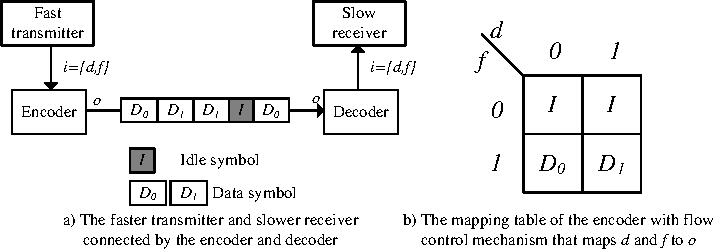
\includegraphics[width=\textwidth]{nonuniq_pred}
\caption{带有流控机制的编码器}
\label{fig_fc}
\end{figure}

\begin{figure}[b]
\centering
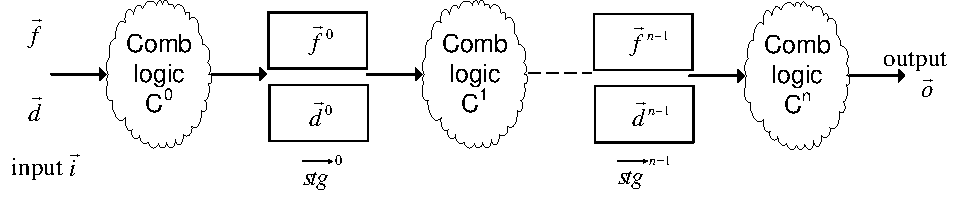
\includegraphics[width=0.9\textwidth]{pipemod1_pred}
\caption{带有流水线和流控机制的编码器}
\label{fig_pipeenc}
\end{figure}



同时,
如图\ref{fig_pipeenc}所示,
许多编码器
包含流水线级$\vec{stg}^j$ 已将关键的数据路径划分为多个子段$C^j$,
这样有助于提高性能。
类似于$\vec{i}$,
每个流水线级$\vec{stg}^j$ 也可以划分为留空向量$\vec{f}^j$ 和数据向量$\vec{d}^j$。

然而由秦et al. 的算法\cite{QinTODAES15} 产生的解码器并不包含流水线。
这使得其运行速度远低于相应的编码器。
为了解决该问题,
本文提出了一个全新的算法以为此类编码器产生带有流控机制和流水线的解码器。
该算法首先使用秦et al. \cite{QinTODAES15}的算法来寻找$\vec{f}$ 并推导$valid(\vec{f})$。
然后分别通过强制和不强制$valid(\vec{f})$,
已从所有寄存器集合中找到每一个寄存器级$\vec{stg}^j$的$\vec{d}^j$ 和$\vec{f}^j$。
最后通过Jiang et al. \cite{InterpBoolFunction}的算法特征化$\vec{stg}^j$ 和$\vec{i}$的布尔函数。

实验结果表明,
该算法能够为多个工业界的真实编码器正确的产生带有流控和流水线的解码器。

本文剩余部分如下组织。
%小节\ref{sec_prem} 介绍相关的背景知识;
小节\ref{sec_framework} 介绍本文算法的整体结构;
小节\ref{sec_pipeinfer} 找到每一个流水线级$\vec{stg}^j$中的$\vec{f}^j$ 和$\vec{d}^j$ 。
小节\ref{sec_char} 为$\vec{stg}^j$ 和$\vec{i}$特征化布尔函数。
小节\ref{sec_exp} 和\ref{sec_conclude} 分别给出实验结果和结论。


%
%\section{背景知识}\label{sec_prem}
%
%% \subsection{Flow control mechanism}\label{subsec_fc}
%
%
%
%\subsection{命题逻辑可满足}\label{subsec_SAT}
%布尔集合记为$\mathbb{B}=\{0,1\}$。
%多个变量组成的向量记为$\vec{v}=(v,\dots)$。
%$\vec{v}$ 中的变量个数记为$|\vec{v}|$。
%若一个变量$v$ 是$\vec{v}$的成员,
%则记为$v\in\vec{v}$;
%否则记为$v\notin\vec{v}$。
%对于一个变量$v$ 和一个向量$\vec{v}$,
%若$v\notin\vec{v}$,
%则一个同时包含$v$ 和所有$\vec{v}$ 的成员的新变量记为$v\cup\vec{v}$。
%若$v\in \vec{v}$,
%则一个包含$\vec{v}$ 的所有成员,但是不包含$v$的
%新变量记为$\vec{v}-v$。
%对于两个向量$\vec{a}$ 和$\vec{b}$,
%则同时包含$\vec{a}$ 和$\vec{b}$ 的所有成员的新向量记为$\vec{a}\cup\vec{b}$。
%
%对于变量集合$V$上的公式$F$,
%其命题逻辑可满足问题(SAT)
%的目的在于巡展赋值函数$A:V\to \mathbb{B}$,
%使得$F$ 能够取值为$1$。
%若$A$ 存在则$F$ 是可满足的;
%否则是不可满足的。
%
%对于两个布尔命题逻辑公式$\phi_A$ 和$\phi_B$,
%若$\phi_A\wedge \phi_B$ 不可满足,
%则存在仅引用$\phi_A$ 和$\phi_B$共同变量的公式$\phi_I$ ,
%使得$\phi_A\Rightarrow \phi_I$
%且$\phi_I\wedge \phi_B$ 不可满足。
%$\phi_I$ 称为$\phi_A$ 相对于$\phi_B$的Craig 插值\cite{Craig} 。
%可以使用McMillan算法 \cite{interp_McMillan} 产生该插值。
%
%
%
%
%\subsection{有限状态机}\label{subsec_fsm}
%
%
%
%编码器使用有限状态机$M=(\vec{s},\vec{i},\vec{o},T)$作为模型,
%其中包含状态向量$\vec{s}$。
%输入向量$\vec{i}$,
%输出向量$\vec{o}$,
%状态迁移函数$T: \vec{s}\times \vec{i}\to \vec{s}\times \vec{o}$
%从当前状态向量和输入向量计算出下一状态向量和输出向量。
%
%$M$ 的行为可以通过展开状态迁移函数进行推导。
%状态变量$s\in\vec{s}$, 输入变量$i\in\vec{i}$ 和输出变量$o\in\vec{o}$ 在上述展开序列的第$n$步中
%分别记为$s_n$, $i_n$ 和$o_n$。
%更进一步的,
%在第$n$步中的状态向量,输入向量和输出向量分别记为$\vec{s}_n$, $\vec{i}_n$ 和$\vec{o}_n$。
%一个路径是一个序列$<\vec{s}_n,\dots,\vec{s}_m>$ 使得对于所有$n\le j< m$,
%有$\exists \vec{i}_j\vec{o}_j (\vec{s}_{j+1},\vec{o}_j)\equiv T(\vec{s}_j,\vec{i}_j)$ 。
%而一个环是一个路径$<\vec{s}_n,\dots,\vec{s}_m>$ 使得$\vec{s}_n\equiv \vec{s}_m$。
%
%
%
%\subsection{寻找$\vec{f}$的停机算法}\label{subsec_chkextdec}
%
%
%秦et al. \cite{QinTODAES15} 提出了一个寻找$\vec{f}$ 的停机算法。
%该算法通过迭代的调用一个sound和一个complete的算法以最终得到收敛的答案。.
%% The first one is an under-approximative one that presented in \ref{subsub_sound},
%% while the second one is an over-approximative one presented in \ref{subsub_complete}.
%% We will present these two approaches below and show
%% that they will eventually converge.
%
%\subsubsection{sound算法}\label{subsub_sound}
%如图\ref{fig_pc}a)所示,
%在展开的迁移关系上,
%一个输入变量$i\in\vec{i}$ 能够被唯一决定,
%是指存在$p$, $l$ 和$r$,
%使得对于输出序列$<\vec{o}_p,\dots,\vec{o}_{p+l+r}>$的每一个取值,
%$i_{p+l}$ 不能同时为0和1。
%折等价于公式(\ref{uniqt1})中的$F_{PC}(p,l,r)$的不可满足性。
%行1 对应于图\ref{fig_pc}a)中的路径,
%而行2 是其拷贝
%行3 强制这两个路径的输出相等。
%而行4 强制$i_{p+l}$ 不等。
%该算法是sound的因为当(\ref{uniqt1}) 不可满足
%$i$ 肯定是$\vec{f}$的成员。
%
%\begin{equation}\label{uniqt1}
%% \begin{split}
%F_{PC}(p,l,r):=
%\left\{
%\begin{array}{cc}
%&\bigwedge_{m=0}^{p+l+r}
%\{
%(\vec{s}_{m+1},\vec{o}_m)\equiv T(\vec{s}_m,\vec{i}_m)
%\}
%\\
%\wedge&\bigwedge_{m=0}^{p+l+r}
%\{
%(\vec{s'}_{m+1},\vec{o'}_m)\equiv T(\vec{s'}_m,\vec{i'}_m)
%\}
%\\
%\wedge&\bigwedge_{m=p}^{p+l+r}\vec{o}_m\equiv \vec{o'}_m \\
%\wedge& i_{p+l}\equiv 1 \wedge  i'_{p+l}\equiv 0
%% \wedge&\bigwedge_{m=0}^{p+l+r}assertion(\vec{i}_m) \\
%% \wedge&\bigwedge_{m=0}^{p+l+r}assertion(\vec{i'}_m)
%\end{array}
%\right\}
%% \end{split}
%\end{equation}
%
%\begin{figure}[t]
%\begin{center}
%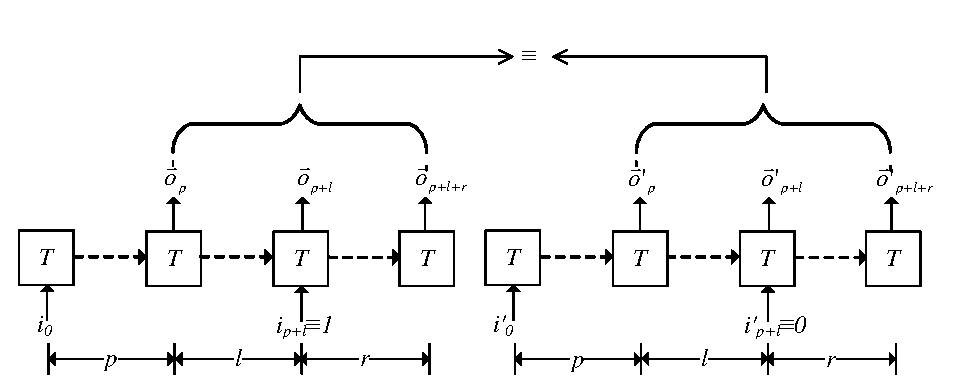
\includegraphics[width=\textwidth]{pc}
%\end{center}
%\caption{sound和complete方法}
%  \label{fig_pc}
%\end{figure}
%
%
%%
%
%
%
%\subsubsection{complete算法}\label{subsub_complete}
%对于上述的$F_{PC}(p,l,r)$ ,
%有两种可能性:
%\textbf{(1)}. 存在$p$, $l$ 和$r$,使得$i_{p+l}$ 能够被$<\vec{o}_{p},\dots,\vec{o}_{p+l+r}>$ 唯一决定;
%或者\textbf{(2)}. $i_{p+l}$ 对于任意$p$, $l$ 和$r$都不能被唯一决定。
%
%
%对于第一种情形,
%通过迭代的增加$p$, $l$ 和$r$,
%$F_{PC}(p,l,r)$ 总能够变成不可满足。
%而对于第二种情形,
%该算法将永不停机。
%因此,
%为了得到一个停机算法,
%我们需要如图\ref{fig_pc}b) 所示的方法去检查第二种情形。
%该方法类似于\ref{fig_pc}a) ,
%但是在三个状态序列$<\vec{s}_{0},\dots,\vec{s}_{p}>$, $<\vec{s}_{p+1},\dots,\vec{s}_{p+l}>$ 和
%$<\vec{s}_{p+l+1},\dots,\vec{s}_{p+l+r}>$上增加了三个约束用于检测环。
%该方法形式化的定义于公式(\ref{uniqln})中。
%其中最后三行即为我们新加的三个约束。
%该方法是complete,
%因为当其是可满足的时候,
%我们可以通过展开
%这三个环来证明第二种情形并断定 $i\notin \vec{f}$。
%
%\begin{equation}\label{uniqln}
%% \begin{split}
%F_{LN}(p,l,r):=\\
%\left\{
%\begin{array}{cc}
%&F_{PC}(p,l,r)\\
%\wedge&\bigvee_{x=0}^{p-1}\bigvee_{y=x+1}^{p} \{\vec{s}_x\equiv \vec{s}_y\wedge \vec{s'}_x\equiv \vec{s'}_y\} \\
%\wedge&\bigvee_{x=p+1}^{p+l-1}\bigvee_{y=x+1}^{p+l} \{\vec{s}_x\equiv \vec{s}_y\wedge \vec{s'}_x\equiv \vec{s'}_y\} \\
%\wedge&\bigvee_{x=p+l+1}^{p+l+r-1}\bigvee_{y=x+1}^{p+l+r} \{\vec{s}_x\equiv \vec{s}_y\wedge \vec{s'}_x\equiv \vec{s'}_y\}
%\end{array}
%\right\}
%% \end{split}
%\end{equation}
%
%
%\subsubsection{通过算法\ref{alg_fofc}找到$\vec{f}$ }\label{subsubsec_findfc}
%
%在行\ref{adduniq},
%所有能够被唯一决定的输入$i$ 将被移到$\vec{f}$。
%若$F_{LN}(p,l,r)$ 在行\ref{nonuniqres}是可满足的,
%所有可满足的输入$i$ 将被移到$\vec{d}$.
%该算法的正确性和停机性证明请见\cite{QinTODAES15} 。
%
%\begin{algorithm}[t]
%\begin{algorithmic}[1]
%\STATE{输入:输入向量$\vec{i}$.}
%\STATE{输出:$\vec{f}\subset \vec{i}$, 在此次搜索中找到的最大$p$, $l$ 和$r$ }
%\STATE $\vec{f}: = \{\}$;$\vec{d}:= \{\}$;$p$:= 0 ;~$l$:= 0 ;~$r$:= 0 \;
%\label{while}\WHILE{$\vec{i}\ne \{\}$}
%  \STATE 假设$i\in\vec{i}$\;
%  \STATE $p++$; ~ $l++$; ~ $r++$\;
%  \IF {$F_{PC}(p,l,r)$ 对于$i$不可满足}
%    \label{adduniq}
%    \STATE $\vec{f}:= i\cup\vec{f}$ ; ~
%    \STATE $\vec{i}:=\vec{i}-i$\;
%  \label{nonuniqres}
%  \ELSIF {$F_{LN}(p,l,r)$ 对于$i$可满足}
%    \STATE $\vec{d}:=i\cup\vec{d}$ ; ~
%    \STATE $\vec{i}:=\vec{i}-i$
%  \ENDIF
%\ENDWHILE
%\RETURN ($\vec{f}$, $p$, $l$, $r$)
%\caption{Identifying the flow control vector $\vec{f}$}
%\label{alg_fofc}
%\end{algorithmic}
%\end{algorithm}
%
%
%
%
%
%\subsection{推导使得$\vec{d}$ 被唯一决定的$valid(\vec{f})$ }\label{subsec_infer}
%
%该算法也是由秦et al. \cite{QinTODAES15}提出的。
%它首先给出算法\ref{alg_craigchar},
%该算法用于特征化一个函数,覆盖所有能够使得一个布尔关系满足的赋值集合。
%然后如图\ref{fig_mono}所示,
%算法\ref{alg_craigchar} 被用于特征化函数$\neg FSAT_{PC}(p,l,r)$,
%$valid(\vec{f})$的单调递增下估计,
%和$\neg FSAT_{LN}(p,l,r)$,
%$valid(\vec{f})$的单调递减上估计。
%最终我们指出这两者将收敛到$valid(\vec{f})$。
%% Please refer to \cite{QinTODAES15} for the proof of its correctness and termination.
%
%
%
%\subsubsection{特征化使得一个布尔关系可满足的布尔函数}\label{subsubsec_craig}
%
%对于一个布尔关系$R(\vec{a},\vec{b},t)$,
%有$R(\vec{a},\vec{b},0)\wedge R(\vec{a},\vec{b},1)$ 不可满足。
%算法\ref{alg_craigchar} 特征化一个布尔寒素$FSAT_R(\vec{a})$,
%该函数覆盖且仅覆盖了能使得
%$R(\vec{a},\vec{b},1)$ 可满足的所有$\vec{a}$。
%行\ref{testsat} 找到$\vec{a}$ 的一个赋值,
%尚未被 $FSAT_R(\vec{a})$ 覆盖而且能够使得$R(\vec{a},\vec{b},1)$ 可满足。
%行\ref{cofact1}, \ref{cofact2} 和\ref{ab} 使用
%McMillan算法\cite{interp_McMillan} 将该赋值放大为$ITP(\vec{a})$。
%行\ref{add} 将$ITP(\vec{a})$ 加入$FSAT_R(\vec{a})$。
%
%
%\begin{algorithm}[t]
%\begin{algorithmic}[1]
%\STATE{输入:布尔关系$R(\vec{a},\vec{b},t)$}
%\STATE{输出:能够使得$R(\vec{a},\vec{b},1)$ 可满足的$FSAT_R(\vec{a})$ }
%\label{initcondition}
%\STATE $FSAT_R(\vec{a}):= 0$ ;
%\label{testsat}
%\WHILE { $R(\vec{a},\vec{b},1)\wedge\neg FSAT_R(\vec{a})$ 可满足}
%  \STATE 假设$A:\vec{a}\cup\vec{b}\cup\{t\}\rightarrow \{0,1\}$ 是一个可满足赋值;
%\label{cofact1}
%  \STATE $\phi_A(\vec{a}):= R(\vec{a},A(\vec{b}),1)$ ;
%\label{cofact2}
%  \STATE $\phi_B(\vec{a}):= R(\vec{a},A(\vec{b}),0)$ ;
%\label{ab}
%  \STATE 假设$ITP(\vec{a})$ 是$\phi_A$ 相对于$\phi_B$ 的Craig插值 ;
%\label{add}
%  \STATE $FSAT_R(\vec{a}):= ITP(\vec{a}) \vee FSAT_R(\vec{a})$ ;
%\ENDWHILE
%\RETURN $FSAT_R(\vec{a})$
%\caption{$CharacterizingFormulaSAT(R,\vec{a},\vec{b},t)$}
%\label{alg_craigchar}
%\end{algorithmic}
%\end{algorithm}
%
%\subsubsection{计算$valid(\vec{f})$的单调递增下估计}\label{subsub_nonloop}
%通过将公式(\ref{uniqt1}) 中的$i$替换为算法\ref{alg_fofc}中推导的$\vec{d}$ ,
%我们有:
%
%\begin{equation}\label{uniqt1d}
%% \begin{split}
%F^d_{PC}(p,l,r):=
%\left\{
%\begin{array}{cc}
%&\bigwedge_{m=0}^{p+l+r}
%\{
%(\vec{s}_{m+1},\vec{o}_m)\equiv T(\vec{s}_m,\vec{i}_m)
%\}
%\\
%\wedge&\bigwedge_{m=0}^{p+l+r}
%\{
%(\vec{s'}_{m+1},\vec{o'}_m)\equiv T(\vec{s'}_m,\vec{i'}_m)
%\}
%\\
%\wedge&\bigwedge_{m=p}^{p+l+r}\vec{o}_m\equiv \vec{o'}_m \\
%\wedge& \vec{d}_{p+l}\ne \vec{d}'_{p+l} \\
%% \wedge&\bigwedge_{m=0}^{p+l+r}assertion(\vec{i}_m) \\
%% \wedge&\bigwedge_{m=0}^{p+l+r}assertion(\vec{i'}_m)
%\end{array}
%\right\}
%% \end{split}
%\end{equation}
%
%% Here,
%% $\vec{d}_{p+l}\ne \vec{d}'_{p+l}$ means some bit in $\vec{d}_{p+l}$
%% isn't equal to the corresponding bit in $\vec{d}'_{p+l}$.
%若$F^d_{PC}(p,l,r)$ 可满足,
%则$\vec{d}_{p+l}$ 不能被$<\vec{o}_p,\dots,\vec{o}_{p+l+r}>$唯一决定。
%通过收集公式 (\ref{uniqt1d})的第三行,
%我们定义$T_{PC}(p,l,r)$ :
%
%\begin{equation}\label{tpc}
%% \begin{split}
%T_{PC}(p,l,r):=\\
%\left\{
%\begin{array}{cc}
%      &\bigwedge_{m=p}^{p+l+r}\vec{o}_m\equiv \vec{o'}_m \\
%\end{array}
%\right\}
%% \end{split}
%\end{equation}
%
%\begin{figure}[b]
%\begin{center}
%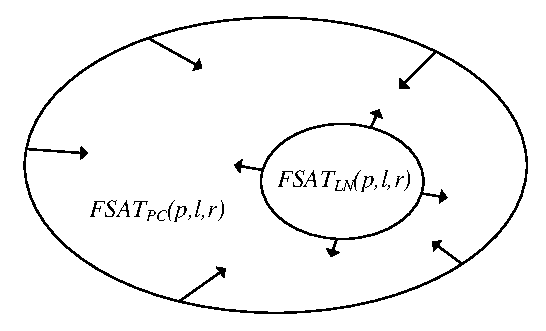
\includegraphics[width=0.5\textwidth]{mono}
%\end{center}
%\caption{The monotonicity of $FSAT_{PC}(p,l,r)$ and $FSAT_{LN}(p,l,r)$}
%  \label{fig_mono}
%\end{figure}
%
%通过将$T_{PC}(p,l,r)$ 替换回$F^d_{PC}(p,l,r)$,
%我们有:
%
%\begin{equation}\label{fpcq}
%% \begin{split}
%F'^d_{PC}(p,l,r,t):=
%\left\{
%\begin{array}{cc}
%&\bigwedge_{m=0}^{p+l+r}
%\{
%(\vec{s}_{m+1},\vec{o}_m)\equiv T(\vec{s}_m,\vec{i}_m)
%\}
%\\
%\wedge&\bigwedge_{m=0}^{p+l+r}
%\{
%(\vec{s'}_{m+1},\vec{o'}_m)\equiv T(\vec{s'}_m,\vec{i'}_m)
%\}
%\\
%\wedge& t\equiv T_{PC}(p,l,r)\\
%\wedge& \vec{d}_{p+l}\ne \vec{d'}_{p+l} \\
%% \wedge&\bigwedge_{m=0}^{p+l+r}assertion(\vec{i}_m) \\
%% \wedge&\bigwedge_{m=0}^{p+l+r}assertion(\vec{i'}_m)
%\end{array}
%\right\}
%% \end{split}
%\end{equation}
%
%
%很明显$F^d_{PC}(p,l,r)$ 和$F'^d_{PC}(p,l,r,1)$ 是等价的,
%我们进一步定义:
%
%\begin{equation}\label{pcdef1}
%\vec{a}:=\vec{f}_{p+l}
%\end{equation}
%
%\begin{equation}\label{pcdef2}
%\vec{b}:=\vec{d}_{p+l}\cup \vec{d'}_{p+l}\cup \vec{s}_0\cup \vec{s'}_0\cup\bigcup_{0\le x\le p+l+r,x\neq (p+l)}(\vec{i}_{x}\cup\vec{i'}_{x})
%\end{equation}
%
%因此,
%向量$\vec{a}\cup\vec{b}$ 包含所有步的输入向量$<\vec{i}_0,\dots,\vec{i}_{p+l+r}>$ 和$<\vec{i'}_0,\dots,\vec{i'}_{p+l+r}>$。
%它同时也包含两个初始状态$\vec{s}_0$ 和$\vec{s'}_0$。
%因此$\vec{a}$ 和$\vec{b}$ 能唯一决定$F'^d_{PC}(p,l,r,t)$中$t$ 的取值。
%这意味着$R(\vec{a},\vec{b},1)\wedge R(\vec{a},\vec{b},0)$ 是不可满足的。
%因此,
%对于$p$, $l$ 和$r$的特定组合,
%在$\vec{f}_{p+l}$ 上定义且能够使$F'^d_{PC}(p,l,r,1)$ 满足的函数可以通过使用$F'^d_{PC}(p,l,r,t)$, $\vec{a}$ 和$\vec{b}$ 调用算法定义如下:
%
%\begin{equation}\label{fsat_pc}
%FSAT_{PC}(p,l,r):=CharacterizingFormulaSAT(F'^d_{PC}(p,l,r,t),\vec{a},\vec{b},t)
%\end{equation}
%
%如图\ref{fig_mono}所示,
%$\neg FSAT_{PC}(p,l,r)$ 是$valid(\vec{f})$ 的针对
%$p$, $l$ 和$r$
%单调递增的下估计。
%% \end{proposition}
%
%
%
%
%\subsubsection{计算$valid(\vec{f})$的单调递减上估计}\label{subsub_loop}
%类似的,
%我们定义:
%
%\begin{equation}\label{tln}
%% \begin{split}
%T_{LN}(p,l,r):=\\
%\left\{
%\begin{array}{cc}
%      &\bigwedge_{m=p}^{p+l+r}\vec{o}_m\equiv \vec{o'}_m \\
%\wedge&\bigvee_{x=0}^{p-1}\bigvee_{y=x+1}^{p} \{\vec{s}_x\equiv \vec{s}_y\wedge \vec{s'}_x\equiv \vec{s'}_y\} \\
%\wedge&\bigvee_{x=p+1}^{p+l-1}\bigvee_{y=x+1}^{p+l} \{\vec{s}_x\equiv \vec{s}_y\wedge \vec{s'}_x\equiv \vec{s'}_y\} \\
%\wedge&\bigvee_{x=p+l+1}^{p+l+r-1}\bigvee_{y=x+1}^{p+l+r} \{\vec{s}_x\equiv \vec{s}_y\wedge \vec{s'}_x\equiv \vec{s'}_y\}
%\end{array}
%\right\}
%% \end{split}
%\end{equation}
%
%
%
%\begin{equation}\label{lndef1}
%F'^d_{LN}(p,l,r,t):=
%\left\{
%\begin{array}{cc}
%&\bigwedge_{m=0}^{p+l+r}
%\{
%(\vec{s}_{m+1},\vec{o}_m)\equiv T(\vec{s}_m,\vec{i}_m)
%\}
%\\
%\wedge&\bigwedge_{m=0}^{p+l+r}
%\{
%(\vec{s'}_{m+1},\vec{o'}_m)\equiv T(\vec{s'}_m,\vec{i'}_m)
%\}
%\\
%% \wedge& \vec{f}_{p+l}\equiv \vec{f'}_{p+l}\\
%\wedge& t\equiv T_{LN}(p,l,r)\\
%\wedge& \vec{d}_{p+l}\ne \vec{d'}_{p+l} \\
%% \wedge&\bigwedge_{m=0}^{p+l+r}assertion(\vec{i}_m) \\
%% \wedge&\bigwedge_{m=0}^{p+l+r}assertion(\vec{i'}_m)
%\end{array}
%\right\}
%\end{equation}
%
%
%\begin{equation}\label{fsat_ln}
%FSAT_{LN}(p,l,r):=CharacterizingFormulaSAT(F'^d_{LN}(p,l,r,t),\vec{a},\vec{b},t)
%\end{equation}
%
%如图\ref{fig_mono}所示,
%$\neg FSAT_{LN}(p,l,r)$ 是$valid(\vec{f})$ 相对于$p$, $l$ 和$r$.的一个单调递减的上估计。
%
%
%
%\subsubsection{使用算法\ref{algo_infer}推导$valid(\vec{f})$ }\label{subsub_overal}
%\begin{algorithm}[t]
%\begin{algorithmic}[1]
%\STATE $p$:= $0$;~$l$:= $0$;~$r$:= $0$ \;
%\WHILE{ $\neg FSAT_{LN}(p,l,r)\wedge FSAT_{PC}(p,l,r)$ 可满足}
%  \STATE $p$ ++ ;~$l$ ++ ;~$r$ ++ ;
%\ENDWHILE
%\RETURN {$\neg FSAT_{LN}(p,l,r)$}
%\caption{推导$valid(\vec{f}_{p+l})$}
%\label{algo_infer}
%\end{algorithmic}
%\end{algorithm}
%
%该算法迭代的增加$p$, $l$ 和$r$,
%直到$FSAT_{PC}(p,l,r)$ 和$FSAT_{LN}(p,l,r)$ 收敛。
%其正确性和停机性见\cite{QinTODAES15} 。


\section{算法框架}\label{sec_framework}


\subsection{编码器的一般性模型}
如图\ref{fig_pipeenc}所示,
我们假设编码器包含$n$ 流水线级$\vec{stg}^j$,
其中$0\le j \le n-1$。
每一个流水线级$\vec{stg}^j$ 能够被进一步划分为流控向量$\vec{f}^j$ 和数据向量$\vec{d}^j$。
而输入向量$\vec{i}$,
和\cite{QinTODAES15}一样,
也能被划分为留空向量$\vec{f}$ 和数据向量$\vec{d}$。
如果将组合逻辑块$C^j$ 视为一个函数,
则该编码器可以使用下列等式定义:

\begin{equation}\label{equ_genpipe}
\begin{array}{cccc}
\vec{stg}^0   & := & C^0(\vec{i})         &\\
\vec{stg}^j   & := & C^j(\vec{stg}^{j-1}) & 1\le j\le n-1\\
\vec{o}       & := & C^n(\vec{stg}^{n-1}) &
\end{array}
\end{equation}


%\begin{figure}[b]
%\begin{center}
%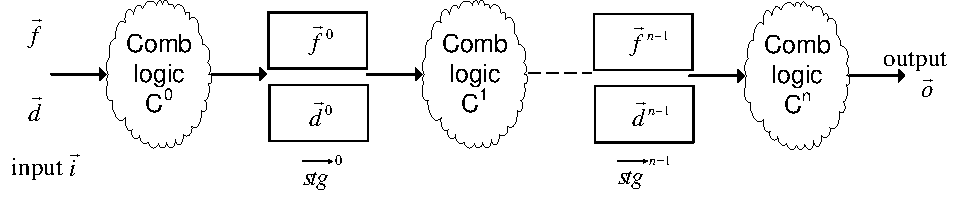
\includegraphics[width=\textwidth]{pipemod1_pred}
%\end{center}
%\caption{包含流水线级和流控机制的一般性编码器模型}
%  \label{fig_pipeenc}
%\end{figure}



在本文中,
上标始终意味着流水线级,
而下标,
如小节\ref{subsec_fsm}指出,
始终意味着在展开的迁移关系序列中的步。
例如,
$\vec{stg}^j$ 是第$j$个流水线级。
而$\vec{stg}^j_i$ 该第$j$流水线级
在第$i$步的取值。

\subsection{算法框架}

基于图\ref{fig_pipeenc}所示的编码器结构,
我们算法的框架为:

\begin{enumerate}
 \item 调用算法\ref{alg_fofc} 以将$\vec{i}$ 划分为$\vec{f}$ 和$\vec{d}$。
 \item 调用算法\ref{algo_infer} 以推导能够使得$\vec{d}$
 被唯一决定的$valid(\vec{f})$和其对应的$p$, $l$ 和$r$。
 \item 在小节\ref{sec_pipeinfer},
 找到每一个流水线级$\vec{stg}^j$中的$\vec{f}^j$ 和$\vec{d}^j$ 。
 \item 在小节\ref{sec_char},
 为每一个流水线级$\vec{stg}^j$
 和输入向量 $\vec{i}$特征化布尔函数。
\end{enumerate}



\section{推导流水线结构}\label{sec_pipeinfer}


\subsection{压缩$r$ 和$l$}\label{reduceing}

\begin{algorithm}[t]
\begin{algorithmic}[1]
\FOR{$r':=r \to 0$}
\label{testr_1}
  \IF{$r'\equiv 0$ or $F_{PC}(p,l,r'-1)\wedge valid(\vec{f}_{p+l})$ 对于某些$i\in \vec{i}$可满足}
    \STATE break
  \ENDIF
\ENDFOR
\RETURN $r'$
\caption{压缩$r$}
\label{algo_remove2}
\end{algorithmic}
\end{algorithm}

由于算法\ref{algo_infer} 同时增加$p$, $l$ 和$r$ ,
因此$l$ 和$r$存在一定程度的冗余。
因此我们需要首先在算法\ref{algo_remove2}中压缩$r$。


在行\ref{testr_1},
我们将推导的谓词$valid(\vec{f})$ 和$F_{PC}(p,l,r'-1)$与在一起。
当该公式可满足时,
则$r'$ 是最后一个使得$F_{PC}(p,l,r')\wedge valid(\vec{f}_{p+l})$ 不可满足的值,
我们将其直接直接返回。
另一方面,
当$r'\equiv 0$,
$F_{PC}(p,l,0)$ 肯定已经在上一个迭代中被测试,
且结果为不可满足。
此时我们直接返回$0$。


这样,
我们从算法\ref{algo_remove2}得到了一个压缩的$r$,
使得$\vec{i}_{p+l}$ 可以被$<\vec{o}_{p},\dots,\vec{o}_{p+l+r}>$唯一决定。

\begin{figure}[t]
\begin{center}
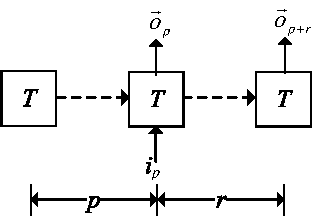
\includegraphics[width=0.5\textwidth]{pc1_pred}
\end{center}
\caption{使用削减的输出序列恢复输入}
  \label{fig_pc1}
\end{figure}

我们进一步要求:
\begin{enumerate}
 \item 如图\ref{fig_pc1}所示,
 $l$ 可以被削减为0。
 这意味着$\vec{i}_{p}$ 可以被$<\vec{o}_{p},\dots,\vec{o}_{p+r}>$唯一决定。
 即所有的未来输出。
 \item 上述的输出序列$<\vec{o}_{p},\dots,\vec{o}_{p+r}>$
 能被进一步压缩为$\vec{o}_{p+r}$。
 这意味着只需$\vec{o}_{p+r}$ 即可唯一决定$\vec{i}_p$。
\end{enumerate}

检验这两个要求等价于
检查$F'_{PC}(p,r)\wedge valid(\vec{f}_{p+l})$的不可满足性
其中$F'_{PC}(p,r)$ 定义如下:

\begin{equation}\label{uniqt11}
% \begin{split}
F'_{PC}(p,r):=
\left\{
\begin{array}{cc}
&\bigwedge_{m=0}^{p+r}
\{
(\vec{s}_{m+1},\vec{o}_m)\equiv T(\vec{s}_m,\vec{i}_m)
\}
\\
\wedge&\bigwedge_{m=0}^{p+r}
\{
(\vec{s'}_{m+1},\vec{o'}_m)\equiv T(\vec{s'}_m,\vec{i'}_m)
\}
\\
\wedge&\vec{o}_{p+r}\equiv \vec{o'}_{p+r} \\
\wedge& i_{p}\equiv 1 \wedge  i'_{p}\equiv 0
% \wedge&\bigwedge_{m=0}^{p+l+r}assertion(\vec{i}_m) \\
% \wedge&\bigwedge_{m=0}^{p+l+r}assertion(\vec{i'}_m)
\end{array}
\right\}
% \end{split}
\end{equation}


该要求看起来远远强于(\ref{uniqt1})。
我们将在实验结果中指出他们总能够满足。



\subsection{推导流水线结构}\label{subsec_inferstage}

现在,
基于上述推导的$p$ 和$r$,
我们将公式(\ref{uniqt11}) 中的$F'_{PC}$推广到下面定义的更广泛的形式。
它能够检查任意变量$v$ 在步$j$
能否被向量$\vec{w}$ 在步$k$唯一决定。
现在$v$ 和$\vec{w}$ 可以使输入,输出或者状态向量。

\begin{equation}\label{uniqt2}
% \begin{split}
F''_{PC}(p,r,v,j,\vec{w},k):=
\left\{
\begin{array}{cc}
&\bigwedge_{m=0}^{p+r}
\{
(\vec{s}_{m+1},\vec{o}_m)\equiv T(\vec{s}_m,\vec{i}_m)
\}
\\
\wedge&\bigwedge_{m=0}^{p+r}
\{
(\vec{s'}_{m+1},\vec{o'}_m)\equiv T(\vec{s'}_m,\vec{i'}_m)
\}
\\
\wedge&\vec{w}_{k}\equiv \vec{w'}_{k} \\
\wedge& v_{j}\equiv 1 \wedge  v'_{j}\equiv 0
% \wedge&\bigwedge_{m=0}^{p+l+r}assertion(\vec{i}_m) \\
% \wedge&\bigwedge_{m=0}^{p+l+r}assertion(\vec{i'}_m)
\end{array}
\right\}
% \end{split}
\end{equation}

很明显,
当$F''_{PC}(p,r,v,j,\vec{w},k)$ 不可满足时,
$\vec{w}_k$ 能唯一决定$v_j$.

对于$0\le j\le n-1$,
在第$j$流水线级$\vec{stg}^j$,
其留空向量$\vec{f}^j$ 包含所有的
能够在第$j-((n-1)-(p+r))$-th 步被$\vec{o}$
在第$p+r$步唯一决定的状态变量$s\in \vec{s}$。
注意在这里不需要约束$valid(\vec{f}_p)$。
这可以形式化的定义为:

\begin{equation}\label{stgn_fj}
\vec{f}^{j} :=
 \left\{
 s\in \vec{s} ~|
\begin{array}{cc}
 F''_{PC}(p,r,s,j-D,\vec{o},p+r)\\
 ~is~unsatisfiable
\end{array}
\right\}
\end{equation}

其中:

\begin{equation}\label{stgn_def}
\begin{array}{ccc}
% S             & := & \vec{s}/\bigcup_{j<k\le n-2}\vec{stg}^{k}\\
D             & := & (n-1)-(p+r)\\
\end{array}
\end{equation}

而在第$j$流水线级$\vec{stg}^j$中的数据向量$\vec{d}^j$
包含能够在第$j-((n-1)-(p+r))$步被
$\vec{o}$ 在第$p+r$步唯一决定的所有$s\in \vec{s}$。
注意这里我们需要强制$valid(\vec{f}_p)$。
这可以被形式化的定义为:

\begin{equation}\label{stgn_dj}
\vec{d}^{j} :=
 \left\{
 s\in \vec{s} ~|
 \begin{array}{cc}
 F''_{PC}(p,r,s,j-D,\vec{o},p+r)\wedge valid(\vec{f}_p)\\
 ~is~unsatisfiable
 \end{array}
\right\}
\end{equation}


\section{特征化流水线级和输入的布尔函数}\label{sec_char}
\subsection{特征化最后一个流水线级的布尔函数}

从公式(\ref{stgn_fj})可知,
每个寄存器$s\in \vec{f}^{n-1}$ 能过被$\vec{o}$ 在第$p+r$步唯一决定。
也就是,
$F''_{PC}(p,r,s,p+r,\vec{o},p+r)$ 不可满足且可以划分为:

\begin{equation}
 \phi_A :=
 \left\{
\begin{array}{cc}
&\bigwedge_{m=0}^{p+r}
\{
(\vec{s}_{m+1},\vec{o}_m)\equiv T(\vec{s}_m,\vec{i}_m)
\}
\\
\wedge& s_{p+r}\equiv 1
\end{array}
\right\}
\end{equation}

\begin{equation}
% \begin{split}
\phi_B :=
\left\{
\begin{array}{cc}
&\bigwedge_{m=0}^{p+r}
\{
(\vec{s'}_{m+1},\vec{o'}_m)\equiv T(\vec{s'}_m,\vec{i'}_m)
\}
\\
\wedge&\vec{o}_{p+r}\equiv \vec{o'}_{p+r} \\
\wedge& s'_{p+r}\equiv 0
% \wedge&\bigwedge_{m=0}^{p+l+r}assertion(\vec{i}_m) \\
% \wedge&\bigwedge_{m=0}^{p+l+r}assertion(\vec{i'}_m)
\end{array}
\right\}
% \end{split}
\end{equation}

因为$F''_{PC}(p,r,s,p+r,\vec{o},p+r)$ 等价于$\phi_A \wedge \phi_B$,
所以$\phi_A \wedge \phi_B$ 不可满足
而$\phi_A$ 和$\phi_B$ 的共同变量集合是$\vec{o}_{p+r}$。

根据文献\upcite{InterpBoolFunction},
$\phi_A$ 相对于$\phi_B$ 的Craig插值$\phi_I$可以被计算出来,
只引用$\vec{o}_{p+r}$,
并且覆盖所有能使$s_{p+r}\equiv 1$的$\vec{o}_{p+r}$ 。
同时,
$\phi_I\wedge \phi_B$ 不可满足
这意味着$\phi_I$ 并不覆盖任何使得$s_{p+r}\equiv 0$的$\vec{o}_{p+r}$ 。

因此,
$\phi_I$ 可以作为
从$\vec{o}$恢复$s\in \vec{f}^{n-1}$的布尔函数。

通过将$F''_{PC}(p,r,s,p+r,\vec{o},p+r)$ 替换为$F''_{PC}(p,r,s,p+r,\vec{o},p+r)\wedge valid(f_p)$,
我们可以类似的特征化恢复$s\in\vec{d}^{n-1}$的布尔函数。

\subsection{特征化恢复其他流水线级的布尔函数}
根据图\ref{fig_pipeenc},
% Similar to last subsection,
$\vec{f}^j$ 在第$j-D$步可以被$\vec{stg}^{j+1}$ 在第$j-D+1$步唯一决定。
因此我们将不可满足公式$F''_{PC}(p,r,s,j-D,\vec{stg}^{j+1},j-D+1)$
划分为下列两个公式:

\begin{equation}
 \phi_A :=
 \left\{
\begin{array}{cc}
&\bigwedge_{m=0}^{p+r}
\{
(\vec{s}_{m+1},\vec{o}_m)\equiv T(\vec{s}_m,\vec{i}_m)
\}
\\
\wedge& s_{j-D}\equiv 1
\end{array}
\right\}
\end{equation}

\begin{equation}
% \begin{split}
\phi_B :=
\left\{
\begin{array}{cc}
&\bigwedge_{m=0}^{p+r}
\{
(\vec{s'}_{m+1},\vec{o'}_m)\equiv T(\vec{s'}_m,\vec{i'}_m)
\}
\\
\wedge&\vec{stg}^{j+1}_{j-D+1}\equiv \vec{stg'}^{j+1}_{j-D+1} \\
\wedge& s'_{j-D}\equiv 0
% \wedge&\bigwedge_{m=0}^{p+l+r}assertion(\vec{i}_m) \\
% \wedge&\bigwedge_{m=0}^{p+l+r}assertion(\vec{i'}_m)
\end{array}
\right\}
% \end{split}
\end{equation}

再一次,
$\phi_A$ 相对于$\phi_B$ 的Craig插值$\phi_I$可以被构造出来,
并用做从$\vec{stg}^{j+1}$恢复$s\in\vec{f}^{j}$的布尔函数。

类似的,
将$F''_{PC}(p,r,s,j-D,\vec{stg}^{j+1},j-D+1)$  替换为
$F''_{PC}(p,r,s,j-D,\vec{stg}^{j+1},j-D+1)\wedge valid(f_p)$ ,
我们能特征化从$\vec{stg}^{j+1}$恢复$s\in\vec{d}^{j}$的布尔函数。

\subsection{特征化从第0级流水线恢复输入向量的布尔函数}

根据图\ref{fig_pipeenc},
$\vec{f}$ 在第$p$步能够被$\vec{stg}^0$ 在第$p$步唯一决定。
$F''_{PC}(p,r,i,p,\vec{stg}^0,p)$ 不可满足并可以划分为以下两个公式:

\begin{equation}
% \begin{split}
\phi_A:=
\left\{
\begin{array}{cc}
&\bigwedge_{m=0}^{p+r}
\{
(\vec{s}_{m+1},\vec{o}_m)\equiv T(\vec{s}_m,\vec{i}_m)
\}
\\
\wedge& i_{p}\equiv 1
% \wedge&\bigwedge_{m=0}^{p+l+r}assertion(\vec{i}_m) \\
% \wedge&\bigwedge_{m=0}^{p+l+r}assertion(\vec{i'}_m)
\end{array}
\right\}
% \end{split}
\end{equation}

\begin{equation}
% \begin{split}
\phi_B:=
\left\{
\begin{array}{cc}
&\bigwedge_{m=0}^{p+r}
\{
(\vec{s'}_{m+1},\vec{o'}_m)\equiv T(\vec{s'}_m,\vec{i'}_m)
\}
\\
\wedge&\vec{stg}^0_p\equiv \vec{stg'}^0_p \\
\wedge& i'_{p}\equiv 0
% \wedge&\bigwedge_{m=0}^{p+l+r}assertion(\vec{i}_m) \\
% \wedge&\bigwedge_{m=0}^{p+l+r}assertion(\vec{i'}_m)
\end{array}
\right\}
% \end{split}
\end{equation}

再一次,
$\phi_A$ 相对于$\phi_B$的Craig插值$\phi_I$
可以被用作从$\vec{stg}^0$恢复$i\in\vec{f}$的布尔函数。

类似的,
通过替换$F''_{PC}(p,r,i,p,\vec{stg}^0,p)$ 为$F''_{PC}(p,r,i,p,\vec{stg}^0,p)\wedge valid(\vec{f}_p)$,
我们可以特征化从$\vec{stg}^0$恢复$i\in\vec{d}$的布尔函数。



\section{实验结果}\label{sec_exp}
我们使用OCaml 语言实现了上述算法,
并使用MiniSat 1.14 \cite{EXTSAT}求解产生的CNF公式。
所有的实验使用一台包含16 个Intel Xeon E5648 2.67GHz处理器,
192GB 内存, 和CentOS 5.4 Linux操作系统的服务器上。

\subsection{比较时间和面积}
表\ref{tab_bench} 给出本文中使用的benchmark。
第2和3分别给出输入,输出和寄存器个数。
第4列给出了将编码器映射至LSI10K 库所得到的面积。
本文中,
所有的面积和延迟使用同样的设置得到。


\begin{table*}[t]
\caption{Benchmark和实验结果}
\begin{tabular}{|c|c|c|c|c|c|c|c|c|c|c|}
\hline
 Names     & \multicolumn{4}{|c|}{编码器}                                        &   \multicolumn{3}{|c|}{\cite{ShenTCAD11}产生}      &   \multicolumn{3}{|c|}{本文产生} \\
           & \multicolumn{4}{|c|}{}                                              &   \multicolumn{3}{|c|}{的解码器}                   &   \multicolumn{3}{|c|}{的解码器} \\\cline{2-11}
           &    \#   &   \#    &面积  & 解码器                                   &运行 &延迟 &面积                                    &运行 &延迟 &面积\\
           & in/out  &  reg    &      &   藐视                                   &时间 &(ns) &                                        &时间 &(ns) &    \\\hline\hline
 pcie      & 10/11   & 23      & 326  &PCIE 2.0 \cite{pcie21}                    &0.37 &7.20 &624                                     &8.08 & 5.89&652 \\\hline
 xgxs      & 10/10   & 16      & 453  &     以太网   clause 48 \cite{IEEE8023_S4}&0.21 &7.02 &540                                     &4.25 & 5.93&829 \\\hline
 t2eth     & 14/14   & 49      & 2252 &    以太网   clause 36 \cite{IEEE8023_S4} &12.7 &6.54 &434                                     &430.4& 6.12&877 \\\hline
scrambler  &64/64    & 58      & 1034 & inserting 01 flipping                    &     \multicolumn{6}{|c|}{no pipeline }\\\cline{1-5}
 xfi       & 72/66   & 72      & 7772 &     以太网   clause 49 \cite{IEEE8023_S4}&     \multicolumn{6}{|c|}{stages found}\\\hline
\end{tabular}\label{tab_bench}
\end{table*}





第6到8列分别给出了论文\cite{ShenTCAD11}的算法产生非流水解码器的运行时间,
以及该解码器的延迟和面积。
而第9到11列分别给出了本文算法的类似信息。

比较第7和10列可知
延迟得到了明显的改善。

一个比较令人惊讶的事实是,
两个最大的benchmarks scrambler 和xfi 并不包含流水线。
我们研究并确认了这一点。
他们的面积如此之大是因为使用了很宽的64到72 位数据路径。

\subsection{PCIE推导的流水线结构}

对于pcie,
存在两个流水线级,
其中包含的流控向量和数据向量如图\ref{tab_pcie}所示。

\begin{table}[t]
\centering
\caption{pcie推导的流水线结构}
\begin{tabular}{|c|c|c|c|}
\hline
                       & input                  & pipeline stage 0          &  pipeline stage 1    \\\hline\hline
流控                   &CNTL\_TXEnable\_P0      & InputDataEnable\_P0\_reg  & OutputData\_P0\_reg[9:0]\\
向量                   &                        &                           & OutputElecIdle\_P0\_reg \\\hline
流控                   &CNTL\_TXEnable\_P0      & InputDataEnable\_P0\_reg  & true \\
谓词                   &                        &                           &  \\\hline
数据                   &TXDATA[7:0]             & InputData\_P0\_reg[7:0]   & \\
向量                   &TXDATAK                 & InputDataK\_P0\_reg       & \\\hline
\end{tabular}\label{tab_pcie}
\end{table}


有一个有趣的事实是流水线级1的数据向量是空集。
而所有的流水线寄存器都被识别成为流控向量。
我们研究了源代码,
发现这些流水线寄存器全部都被直接送给输出向量。
因此他们很明显都能够被$\vec{o}$唯一决定。
伊霓裳这并不影响所产生的解码器的正确性。



\subsection{xgxs推导的流水线结构}


对于xgxs,
只有一级流水线,
其中的流控和数据向量如图\ref{tab_xgxs}所示。

\begin{table}[b]
\centering
\caption{xgxs推导的流水线结构}
\begin{tabular}{|c|c|c|}
\hline
                       & input                  &  pipeline stage 0    \\\hline\hline
流控向量               &bad\_code               & bad\_code\_reg\_reg\\\hline
流控谓词               &!bad\_code              & !bad\_code\_reg\_reg \\\hline
数据向量               &encode\_data\_in[7:0]   &ip\_data\_latch\_reg[2:0] \\
                       &konstant                &plus34\_latch\_reg     \\
                       &                        &data\_out\_latch\_reg[5:0]\\
                       &                        &konstant\_latch\_reg   \\
                       &                        &kx\_latch\_reg         \\
                       &                        &minus34b\_latch\_reg   \\\hline
\end{tabular}\label{tab_xgxs}
\end{table}


\subsection{t2ether推导的流水线结构}


\begin{table}[t]
\centering
\caption{t2ether推导的流水线结构}
\begin{tabular}{|c|c|c|c|c|c|}
\hline
                       & input                        & pipeline                  &  pipeline          &  pipeline       &  pipeline               \\
                       &                              & stage 0                   &  stage 1           &  stage 2        &  stage 3                \\\hline\hline
流控                   & tx\_enc\_ctrl\_sel[3:0]      &qout\_reg\_0\_8            & qout\_reg\_0\_9    &qout\_reg[9:0]\_2&qout\_reg[7:1]\_3        \\
向量                   &                              &qout\_reg\_2\_4            & qout\_reg\_1\_5    &                 &qout\_reg\_8\_1          \\
                       &                              &qout\_reg\_1\_4            & qout\_reg\_2\_5    &                 &qout\_reg\_9\_1          \\
                       &                              &                           & qout\_reg\_0\_10   &                 &qout\_reg\_3\_4          \\
                       &                              &                           &                    &                 &qout\_reg\_0\_4          \\
                       &                              &                           &                    &                 &qout\_reg\_3\_5          \\
                       &                              &                           &                    &                 &qout\_reg\_0\_7          \\
                       &                              &                           &                    &                 &sync1\_reg1              \\
                       &                              &                           &                    &                 &sync1\_reg               \\
                       &                              &                           &                    &                 &Q\_reg1                  \\
                       &                              &                           &                    &                 &Q\_reg                         \\\hline
数据                   &txd[7:0]                      &qout\_reg[7:0]             &qout\_reg[7:0]\_1   &                 &                         \\
向量                   &                              &                           &                    &                 &                         \\\hline
\end{tabular}\label{tab_t2ether}
\end{table}


对于t2ether,
有3级流水线,如图\ref{tab_t2ether}所示。
流控谓词比较复杂,
因此我们将他们单独列在下面而不是图\ref{tab_t2ether}中。
输入流控谓词$f$ 为:
\begin{multline}
\begin{array}{l}
( tx\_enc\_ctrl\_sel[2]~\&~tx\_enc\_ctrl\_sel[3] ) | \\
( tx\_enc\_ctrl\_sel[2]~\&~!tx\_enc\_ctrl\_sel[3]~\&~!tx\_enc\_ctrl\_sel[0]~\&~tx\_enc\_ctrl\_sel[1] ) | \\
( !tx\_enc\_ctrl\_sel[2]~\&~tx\_enc\_ctrl\_sel[3] ) | \\
( !tx\_enc\_ctrl\_sel[2]~\&~!tx\_enc\_ctrl\_sel[3]~\&~tx\_enc\_ctrl\_sel[0] )
\end{array}
\end{multline}

第零级流控谓词$valid(\vec{f}^0)$ :
\begin{multline}
\begin{array}{l}
( qout\_reg\_2\_4~\&~qout\_reg\_1\_4~\&~!qout\_reg\_0\_8) | \\
( !qout\_reg\_2\_4~\&~qout\_reg\_0\_8)
\end{array}
\end{multline}

第一级流控谓词$valid(\vec{f}^1)$ 为:

\begin{multline}
\begin{array}{l}
( qout\_reg\_2\_5~\&~qout\_reg\_1\_5~\&~qout\_reg\_0\_10~\&~!qout\_reg\_0\_9) | \\
( qout\_reg\_2\_5~\&~qout\_reg\_1\_5~\&~!qout\_reg\_0\_10) | \\
( qout\_reg\_2\_5~\&~!qout\_reg\_1\_5~\&~!qout\_reg\_0\_10) | \\
( !qout\_reg\_2\_5~\&~qout\_reg\_0\_10~\&~qout\_reg\_0\_9) | \\
( !qout\_reg\_2\_5~\&~!qout\_reg\_0\_10)
\end{array}
\end{multline}


最后两级的流控谓词$valid(\vec{f}^2)$ 和$valid(\vec{f}^3)$ 均为$true$。






%\section{相关工作}\label{sec_relwork}
%
%\subsection{对偶综合}\label{subsec_compsyn_relat}
%第一个对偶综合算法由沈\upcite{ShenICCAD09}提出。
%他通过迭代的展开迁移函数来检查解码器的存在性,
%并通过遍历所有的输出向量取值来特征化解码器的布尔函数。
%其主要弱点在于该算法不停机,
%而且特征化解码器函数时速度太慢。
%
%沈et al.\upcite{ShenTCAD11} 和Liu et al.\upcite{LiuICCAD11} 通过在状态序列上搜索环来解决停机问题。
%而\upcite{ShenTCAD12,LiuICCAD11} 通过Craig插值\upcite{interp_McMillan}高效的特征化解码器函数。
%
%沈et al.\upcite{ShenTCAD12} 自动推导使得解码器存在的配置断言。
%
%秦et al. \upcite{QinTODAES15}
%提出了第一个能处理流控机制的对偶综合算法。
%
%Tu 和Jiang \upcite{TuDAC13} 提出了一个突破性的算法以在恢复编码器输入时考虑其非限界的历史。
%
%
%\subsection{程序取反}\label{subsec_proinv}
%根据Gulwani \upcite{dim_syn},
%程序取反意味着为
%特定程序$P$
%生成一个具有反功能的程序$P^{-1}$。
%因此,
%程序取反非常类似于我们的对偶综合。
%
%最早的程序取反算法基于proof的算法\upcite{prog_inv},
%只能处理非常小的程序和非常简单的语法。
%
%Gl\"{u}ck et al. \upcite{mtd_autoProginv} 取反一阶函数语言的程序,
%通过基于LR的算法来去除非确定性。.
%然而使用函数语言使得其应用场景和我们有很大的差别。
%
%Srivastava et al. \upcite{prog_inv_rev,program_inversion} 假设反程序和原始程序的结构是类似的,
%因此可能的反程序结构可以通过挖掘原始程序中的谓词,表达式和控制流得到。
%这和本文发掘流水线级和流控机制类似。
%该算法迭代的去掉不满足要求的解空间直至剩下正确的解。


\section{结论}\label{sec_conclude}
本文提出了第一个能同时处理流控机制和流水线的对偶综合算法。
实验结果表明本文算法总能够正确的产生带有流控机制和流水线的解码器。


% !Mode:: "Tex:UTF-8"
\chapter{原型系统的实现}
\label{chap:7}
本章针对本文中实现的各个算法的原型系统,
描述他们的整体结构,
各个子系统的功能,
以及这些子系统相互之间的关系和流程。

\section{整体结构}



\begin{figure}[t]
\centering
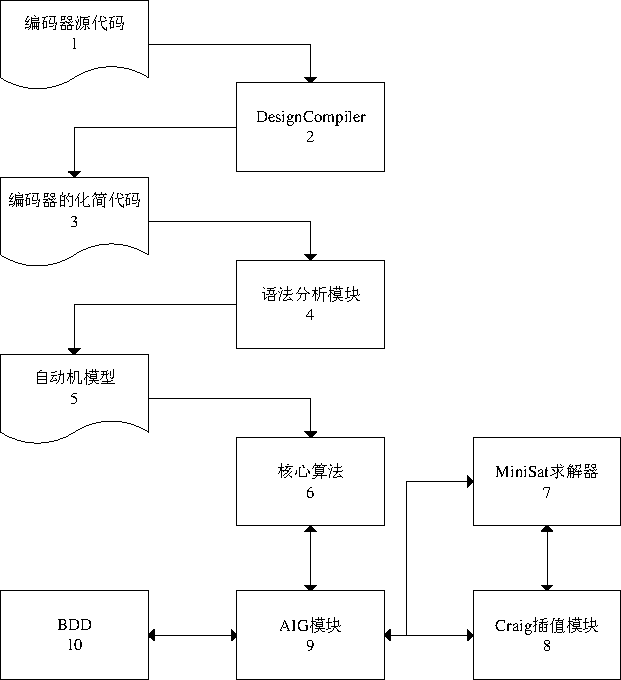
\includegraphics[width=0.8\textwidth]{sysarch}
\caption{原型系统的结构}
\label{fig_sysarch}
\end{figure}

原型系统的结构如图\ref{fig_sysarch}所示。
其中核心算法可以是前述的三个算法,包括:
\begin{enumerate}
\item 第\ref{chap:4}章的面向流控机制的对偶综合算法。
\item 第\ref{chap:5}章的面向流水线的对偶综合算法。
\item 第\ref{chap:6}章的面向流控和流水线的对偶综合算法。
\end{enumerate}


上述三个算法虽然内部结构各不相同,
但是他们与其他各个子系统的关系是完全一样的,
都如图\ref{fig_sysarch}所示。

以下各个小节中我们将详细描述各个子系统的功能。

\subsection{使用DesignCompiler产生编码器的化简代码}

设计编码器的工程师在编写代码的时候,
为了追求更强的表达能力,
更紧凑的代码,
或者更好的可读性等原因,
会使用Verilog语言\upcite{Verilog}提供的各种复杂语法结构。
而开发一个能分析完整的Verilog语法结构的语法分析器会导致大量不必要的额外工作。

因此,
我们选择使用DesignCompiler工具\upcite{DesignCompiler}中自带的完整语法分析器来分析复杂的源代码。

然后我们在DesignCompiler中,
将语法分析的结果映射到DesignCompiler自带的LSI10K单元库中。
为了在保持语义的前提下进一步简化分析结果的语法形式,
我们限制在该映射过程中只能使用与门和非门两种组合逻辑单元。

然后我们将映射的结果导出为一个相对较大,
但是结构非常简单的Verilog源代码文件。
其中只包含一种与门,一种非门和一种寄存器。
这就极大的简化了后继的语法分析程序的设计。


\subsection{语法分析模块}
我们使用OCaml语言自带的词法分析工具OCamllex和语法分析工具OCamlyacc,
创建了针对上述简化的编码器代码的词法和语法分析程序。
词法分析程序的代码在\url{https://github.com/shengyushen/compsyn/blob/master/vp/share/very.mll}。
而语法分析程序的代码在\url{https://github.com/shengyushen/compsyn/blob/master/vp/share/parser.mly}。

分析的结果将被转换为一个有向图$(V,E)$。
其中$V$是节点集合,包含以下类型的节点:
\begin{enumerate}
\item 输入变量$i\in\vec{i}$,
包含1个输出;
\item 输出变量$o\in\vec{o}$,
包含一个输入;
\item 与门,
包含两个输入(A,B)和一个输出Z;
\item 非门,
包含一个输入A和一个输出Z;
\item 寄存器,
包含一个输入D和一个输出Q;
\end{enumerate}

而每条边$e\in E$是单向的,
从一个节点的输出指向另一个节点的输入。
如图\ref{fig_dag}所示。


\begin{figure}[t]
\centering
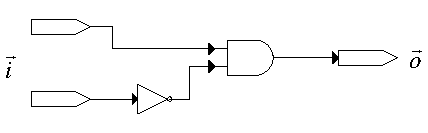
\includegraphics[width=0.8\textwidth]{dag}
\caption{自动机模型的简化描述的例子}
\label{fig_dag}
\end{figure}


\subsection{AIG模块}

AIG是And-Inverter graph的缩写,
即如图\ref{fig_dag}所示的电路结构。
该模块用于构造和维护AIG数据结构,
并负责从AIG到CNF公式的转换。

\subsection{MiniSat求解器}

MiniSat求解器\upcite{EXTSAT}是目前应用最为广泛的SAT求解器。
目前尽管已经有不少新的求解器在性能上超过了MiniSat,
但是由于MiniSat在结构的模块化和可修改性方面具有显著优势,
因此被大量用作理论相关求解器的基础,如数组、未解释函数和线性等式/不等式等。

基于同样的原因,
MiniSat提供了从其自身的C语言内核到OCaml语言的接口。
这为我们在对偶综合算法中调用MiniSat求解器,
并获取其求解结果提供了很大的便利。

\subsection{BDD}
我们选择了学术界广泛使用,
并经过长期验证的CUDD软件包\upcite{cudd}来处理BDD数据结构。
主要应用于小节\ref{sec_bdd_simp}中描述的基于BDD的化简算法。


\subsection{Craig插值模块}
该模块使用MiniSat求解器的Ocaml接口,
以得到不可满足公式的不可满足证明。
并依据小节\ref{sec_craigimp}中定义\ref{def_gencraig}描述的过程产生Craig插值。

\section{主要流程}
我们在图\ref{fig_sysarch}中的每个方框中都标注了数字,
在以下小节的各个主要流程中,
我们将使用这些数字来指出流程中各个步骤及其顺序。

\subsection{语法分析和有限状态机的构造}
该流程以原始的编码器源代码为输入,
经过$1\to 2\to 3\to 4\to 5$,
最后将产生的有限状态机模型送入核心算法模块。

\subsection{SAT求解}
该步骤从核心算法模块开始,
调用AIG模块产生CNF公式,
送入MiniSat求解器,
并返回结果至核心算法。
经过步骤为$6\to 9\to 7\to 9\to 6$。

\subsection{Craig插值}
该步骤从核心算法模块开始,
调用AIG模块产生CNF公式,
送至Craig插值模块产生相应的不可满足公式。
然后送到MiniSat求解器求解并返回不可满足证明。
然后在Craig插值模块中产生插值结果,
最后返回核心算法。
经过步骤为$6\to 9 \to 8 \to 7 \to 8 \to 9 \to 6$。


\subsection{基于余因子和Craig插值的迭代}
此步骤相当于重复的执行上述的Craig插值操作。
即重复的经过8和7,
形成如$6\to 9 \to (8 \to 7 \to)^{+} 8 \to 9 \to 6$的路径。

在完成上述流程之后,
还需要额外调用BDD模块进行结果的化简。

\section{结论}\label{hahahahah}
本章详细描述了系统实现的整体结构,
每个子系统的功能,
以及相互之间的关系。

% !Mode:: "Tex:UTF-8"
\chapter{结束语}
\label{chap:8}
本章对全文进行总结,并对进一步研究工作进行展望。

\section{工作总结}
对偶综合是集成电路设计,
尤其是面向通讯和多媒体芯片设计研究中的重要问题。
本文针对现代通讯协议的编码器中广泛采用的流水线和流控机制,
以提高所产生的解码器的性能和对环境的适应性为研究目标,
系统地研究了对偶综合中的一些重要问题。
具体而言,本文主要对以下几个重要问题进行了深入研究。

第一,研究了基于余因子(Cofactoring)和Craig插值\upcite{Craig}的迭代特征化算法。
在发掘编码器内部结构和自动产生解码器的过程中,
一个必须而且对性能要求非常苛刻的步骤,
是特征化满足特定命题逻辑关系$R$的布尔函数$f$。
传统的算法包括基于SAT或BDD的完全解遍历和和量词削减。
然而这些算法通常受到解空间不规则的困扰,
导致性能低下。
为此,
我们创造性的提出了一个迭代的特征化算法框架。
在每一次迭代中,
为每一个尚未被遍历的解$A$,
利用其对应的余因子化简$R$以满足产生Craig插值要求。
而该插值是$A$的一个充分扩展。
该迭代过程是停机的,
且其性能比传统的完全解遍历算法有巨大的提升。

第二,研究了针对流控机制的对偶综合算法。
传统对偶综合算法的\upcite{ShenICCAD09,ShenTCAD10,DBLP:conf/fmcad/ShenQZL10,ShenTCAD11,ShenICCAD11,ShenTCAD12,LiuICCAD11,LiuTCAD12,TuDAC13}的一个基本假设是,
编码器的输入变量$\vec{i}$总能够被输出变量$\vec{o}$的一个有限长度序列唯一决定。
基于该假设方可构造满足Craig插值的不可满足公式。
然而,
许多高速通讯系统的编码器所带有流控机制\upcite{flowcontrol},
直接违反了上述假设。
该机制将$\vec{i}$划分为有待编码的数据向量$\vec{d}$和用以表达$\vec{d}$有效性的流控向量$\vec{f}$,
并在$\vec{f}$上定义一个有效性谓词$valid(\vec{f})$。
只有在$valid(\vec{f})\equiv 1$的情形下,
$\vec{d}$才能够被$\vec{o}$唯一决定。
为此,
我们创造性的提出了能够处理流控机制的对偶综合算法:
\textbf{首先},
它使用经典的对偶综合算法\upcite{ShenTCAD11}
以识别那些能够被唯一决定的输入变量,
并称他们为流控变量$\vec{f}$。
而其他不能被唯一决定的变量称为数据变量$\vec{d}$。
\textbf{第二},该算法推导一个充分必要谓词$valid(\vec{f})$使得$\vec{d}$能够被
输出变量$\vec{o}$的一个有限长度序列唯一决定。
\textbf{第三},
对于每一个流控变量$f\in\vec{f}$,
该算法使用Craig插值算法\upcite{interp_McMillan}特征化其解码器函数。
同时,
对于数据变量$\vec{d}$,
他们的值只有在$valid(\vec{f}) \equiv 1$时才有意义。
因此每个$d\in\vec{d}$的解码器函数可以类似的使用Craig插值算法得到,
唯一的不同在于必须首先应用谓词$valid(\vec{f}) \equiv 1$。



第三,研究了针对流水线结构的对偶综合算法。
现代集成电路中的编码器,
为了提升工作频率,
通常包含多个流水线级,
以将关键的数据路径划分为多级。
而传统的对偶综合算法\upcite{ShenICCAD09,ShenTCAD10,DBLP:conf/fmcad/ShenQZL10,ShenTCAD11,ShenICCAD11,ShenTCAD12,LiuICCAD11,LiuTCAD12,TuDAC13}
完全无视这种流水线结构,
从而导致生成的解码器无法保持和编码器匹配的频率和性能。
为此,
我们创造性的提出了能够产生流水解码器的对偶综合算法:
首先将传统对偶综合算法推广到非输入输出情形,
以找到编码器中每一个流水线级$\vec{stg}^j$中的寄存器集合;
然后使用迭代Craig插值算法特征化每一个流水线级$\vec{stg}^j$的布尔函数,
以从下一个流水线级$\vec{stg}^{j+1}$ 或输出$\vec{o}$之中恢复$\vec{stg}^j$。
最终特征化$\vec{i}$的布尔函数以从
第一个流水线级$\vec{stg}^0$中恢复$\vec{i}$。

第四,结合上述研究成果,研究了能够同时处理流控和流水线结构的对偶综合算法。
该算法首先使用秦et al. \upcite{QinTODAES15}的算法来寻找$\vec{f}$ 并推导$valid(\vec{f})$。
然后分别通过强制和不强制$valid(\vec{f})$,
已从所有寄存器集合中找到每一个寄存器级$\vec{stg}^j$的$\vec{d}^j$ 和$\vec{f}^j$。
最后通过Jiang et al. \upcite{InterpBoolFunction}的算法特征化$\vec{stg}^j$ 和$\vec{i}$的布尔函数。

综上所述,
本文对基于白盒模型的对偶综合算法中若干关键问题进行了深入的研究,
提出了针对流控和流水线结构的解决方案。
理论分析和实验结果验证了所提出算法的有效性和性能,
对于进一步促进对偶综合算法的发展和应用具有一定的理论意义和应用价值。

\section{研究展望}
近两年来,
随着 100G以太网\upcite{ether100g},128G光纤通道\upcite{fc}和InfiniBand EDR\upcite{InfiniBand}的出现,
单通道传输带宽达到 25~32Gbps。
从而导致高频衰减在标准的背板传输距离上超过了 30dB,
并使其无法达到以太网标准要求的 $10^{-12}$ 误码率\upcite{fecopt}。
而工业界最新的实验性 56Gbps串行传输技术仅能在 11 英寸以内的距离上保证 $10^{-12}$误码率\upcite{nrz56g}。
为了克服上述误码率问题,
基于有限域(Galois field)\upcite{gfbook}的前向纠错编码(FEC)\upcite{fec}被广泛采用于100G以太网\upcite{ether100g}、128G光纤通道\upcite{fc}和InfiniBand EDR\upcite{InfiniBand}等全新的传输标准中。
该纠错机制的特点及其对目前的对偶综合算法的挑战如下:

1. 前向纠错编码设计者和集成电路工程师之间在知识背景和抽象层次上的差异,
导致无法很好的协作完成纠错码的集成电路实现。
一方面,
前向纠错编码设计者专注于有限域等抽象数学领域,
使用诸如singular\upcite{singularbook}等数学工具,
在抽象数学的层面上对FEC进行推理。
然而,
将上述抽象的数学对象映射到集成电路的寄存器传输级描述的工作,
需要由集成电路工程师完成。
而后者关注的是流水线分级、布尔逻辑功能和物理时序等工程细节。
这种知识背景和抽象层次上的差异,
有可能在前向纠错编码(FEC)的集成电路实现上产生潜在的缺陷。
因此就带来了在寄存器传输级上,
对前向纠错编码(FEC)进行形式化验证和对偶综合的强烈需求。

2. 前向纠错编码(FEC)中的有限域算术操作无法使用布尔逻辑推理引擎进行高效推理。
包括对偶综合在内的绝大多数形式化方法依赖于高效的布尔逻辑推理引擎,
包括命题逻辑可满足求解器(SAT)\upcite{DBLP:conf/dac/MoskewiczMZZM01}和二叉判决图(BDD)\upcite{DBLP:journals/tc/Bryant86}。
而在将有限域算术操作映射到布尔逻辑的过程中,
会产生大量的异或操作。
这极大的削弱了SAT和BDD的效率。
近年来致力于验证纠错编码的多篇论文均指出了这一点\upcite{ShenTCAD10,TuDAC13,DBLP:conf/fmcad/LvovLPSE12,DBLP:journals/fmsd/LvovLTPSE14}。

3. 前向纠错编码(FEC)中的长帧将导致对偶综合的巨大运算开销。
现有的对偶综合算法\upcite{ShenICCAD09,ShenTCAD10,DBLP:conf/fmcad/ShenQZL10,ShenTCAD11,ShenTCAD12,ShenICCAD11,LiuICCAD11,LiuTCAD12,TuDAC13}通过逐步的扩大迁移关系的展开长度,
以找到一个特定大小的移动窗口,
使得该窗口内的输出序列能够唯一决定当前的输入字符。
在我们使用的多个工业界标准编码器中,
该窗口大小均不超过 5。
然而在FEC中,
为了尽量减小校验码所占用的带宽,
通常会选择很长的FEC帧尺寸。
比如在IEEE 802.3bj定义的 100G以太网中\upcite{ether100g},
每个FEC帧包含 5280 个比特。
在典型的 250~260 位数据路径宽度上,
这将导致移动窗口的尺寸至少为 20。
这超出了目前为止所有对偶综合算法的处理能力。


4. 前向纠错编码(FEC)的非对称结构和阻塞式的解码算法,
导致现有的对偶综合算法无法产生规则而高效的解码器结构。
正如我们将在下文中指出的,
FEC 解码算法的复杂性远比编码高得多,
而且并不存在线性流水线式的实现,
必须在一个完整的 FEC 帧上经过多次迭代处理方能完成。
这和我们现有对偶综合框架中,
对解码器结构的线性流水线假设有很大区别。

应对并解决这些困难和挑战,
将极大的推进 FEC 的形式化验证和对偶综合方面的研究,
并进而提升面向通讯和多媒体的集成电路芯片设计质量。


% !Mode:: "Tex:UTF-8"
%%% Local Variables:
%%% mode: latex
%%% TeX-master: "../main"
%%% End:

\begin{ack}
值此成文之际,谨向在我攻读博士期间给予我指导、关心、支持和帮助的老师、领导、同学和亲人们致以衷心的感谢!

首先,衷心感谢我的导师贾焰老师为我提供宝贵的学习机会!在课题选择和问题解决过程中,以敏锐的学术洞察力和深厚的科研经验,高屋建瓴地为我论证把关。您在百忙之中仍抽出时间对我的课题进行指导,及时为我解决困难和提供帮助。没有您的指导和帮助,我的研究工作将不可能顺利完成。贾老师对我的言传身教将使我终身受益,您严谨的治学作风、高深的学术造诣、忘我的工作态度和勇攀高峰的精神将永远影响和激励着我。

衷心感谢学院廖湘科老师,工程中心吴庆波老师、戴华东老师、李佩江政委和孔金珠老师为我提供宽松的科研环境,有效保证了我博士课题的研究时间,使我的研究工作能够顺利进行。

衷心感谢我的师姐韩伟红老师!在整个博士课题研究过程中,韩师姐始终给予我热情的指点与帮助,使我的研究工作能够顺利进行。韩师姐严谨的工作态度、细致入微的方法指导,无不使我深感敬佩并始终将师姐作为我学习的榜样。您在生活中给与了我无微不至的关怀,您的热情大方、细心体贴和乐观开朗时刻温暖和鼓励着我。

衷心感谢颜跃进、杨沙洲、刘晓健、汪黎等同事,你们在工程实践和课题研究过程中都提出了良好的建议。
感谢唐晓东、陈松政、魏立峰、何连跃、阳国贵、任怡、董攀、邵立松、马俊、易晓东、高珑、谭郁松、王小川、张卫华等同事,大家勤奋投入的工作态度和超强的科研与工程能力一直都是我学习的目标,与大家并肩奋斗的日子使我得到了良好的锻炼,对今后遇到的任何困难都能够从容面对。

衷心感谢曾经一起战斗过的同事丁滟,你始终如一的勤奋给与我很多的激励。
感谢李姗姗、刘晓东、林斌、鲁晓佩、郑思等廖们的师妹师弟们,
你们朝气蓬勃、思维活跃,参加你们的讨论会,使我开阔了视野。
感谢博士生队的李小芳、周静、阳柳、王晓斌等同学,尽管接触的机会并不太多,
但是每次有困难的时候总能得到同学们的援手,非常感谢。

感谢学院、学员大队、学员队各级领导对我的教育、关心和帮助,你们的辛勤工作为我们创造了良好的学习和生活环境。

特别感谢我的家人。
感谢沈胜宇,与你的每一次交流,都是一场大考,让我得以从固有思维中解放出来,对科学研究有了进一步的认识,从追求一个个小目标开始,逐渐品尝到科研中蕴含的各种滋味,并达到最终的目标。
感谢我的儿子,你的笑容是我最大的安慰,让我在失落中重新拾起勇气;你的懂事和成长给与我力量,激励着我,无论道路如何坎坷我都会坚持走下去。

特别感谢含辛茹苦将我抚育成人并始终宽容待我,随时为我提供无私帮助的父母亲和我的姐姐,对你们的感激之情无法用语言来表达,在我多年的求学和工作之路上,你们始终给与我全身心的支持和关爱。我无法在生活上给与你们照顾,唯有在将来的工作中刻苦努力、做出更大的成绩,以报答你们的养育之恩。祝愿你们永远健康幸福!
\end{ack}


\cleardoublepage
\phantomsection
\addcontentsline{toc}{chapter}{参考文献}
\bibliographystyle{bstutf8}
\bibliography{ref/refs}




% !Mode:: "Tex:UTF-8"
\begin{resume}

  \section*{发表的学术论文} % 发表的和录用的合在一起

  \begin{enumerate}[{[}1{]}]
  \addtolength{\itemsep}{-.36\baselineskip}% 缩小条目之间的间距,下面类似
  \item Qin Y, Shen S, Wu Q, et al. Complementary Synthesis for Encoder with Flow
Control Mechanism [J]. accepted by ACM Transactions on Design Automation of
Electronic Systems.(SCI检索,WOS:xxx,IDS:xxx)

  \item Qin Y, Shen S, Wu Q, et al.Complementary Synthesis for Pipelined Encoder.
accepted by Asia Pacific Design Automation Conference,2016.(EI检索,WOS:xxx,IDS:xxx)

  \item Qin Y, Shen S, Wu Q, et al.Complementary Synthesis for Encoders with
Pipeline and Flow Control Mechanism.
accepted by Haifa Verification Conference,2015.(EI检索,WOS:XXX,IDS:XXX)

  \item Ying Qin, ShengYu Shen, Jingzhu Kong, Huadong Dai:
Cloud-Oriented SAT Solver Based on Obfuscating CNF Formula. APWeb Workshophs 2014: 188-199(EI检索)

  \item Ying Qin, ShengYu Shen, Yan Jia:
Structure-aware CNF obfuscation for privacy-preserving SAT solving. MEMOCODE 2014: 84-93(EI检索)

  \item Shen S, Qin Y, Wang K, et al. Synthesizing Complementary Circuits Automatically
[J/OL]. IEEE Transactions on Computer-Aided Design of Integrated Circuits
and Systems. 2010, 29 (8): 29:1191–29:1202. (SCI检索,WOS:xxx,IDS:xxx)

  \item Shen S, Qin Y, Xiao L, et al. A Halting Algorithm to Determine the Existence of
the Decoder [J/OL]. IEEE Transactions on Computer-Aided Design of Integrated
Circuits and Systems. 2011, 30 (10): 30:1556–30:1563.(SCI检索,WOS:xxx,IDS:xxx)

  \item Shen S, Qin Y, Wang K, et al. Inferring Assertion for Complementary Synthesis
[J/OL]. IEEE Transactions on Computer-Aided Design of Integrated Circuits
and Systems. 2012, 31 (8): 31:1288–31:1292.(SCI检索,WOS:xxx,IDS:xxx)


  \item Shen S, Qin Y, Zhang J. Inferring assertion for complementary synthesis [C/OL]. In
Proceedings of the 2011 International Conference on Computer-Aided Design. San
Jose, CA, USA, 2011: 404–411. (EI检索,WOS:XXX,IDS:XXX)


  \end{enumerate}

  \section*{申请专利} % 有就写,没有就删除
  \begin{enumerate}[{[}1{]}]
  \addtolength{\itemsep}{-.36\baselineskip}%
  \item 董德尊, 鲁晓佩, 廖湘科, 赖明澈, 陆平静, 王绍刚, 徐炜遐, 肖立权, 庞征斌等. 基于多维尺度变换的虫洞拓扑识别方法 (专利号:201310057009)
  \item 李姗姗, 廖湘科, 刘晓东, 吴庆波, 戴华东, 彭绍亮, 王蕾, 付松龄, 鲁晓佩, 郑思. 一种基于图形处理单元的影响最大化并行加速方法(专利号:201210248732.3)
  \end{enumerate}

  \section*{参与主要科研项目} % 有就写,没有就删除
  \begin{enumerate}[{[}1{]}]
  \addtolength{\itemsep}{-.36\baselineskip}%
  \item 国家自然科学基金“面向通讯应用的自动对偶综合方法研究”(项目编号:61070132)
  \end{enumerate}
\end{resume}

%% 最后,需要的话还要生成附录,全文随之结束。
%\appendix
%\backmatter
%%% !Mode:: "Tex:UTF-8"
% TeX
\chapter{模板提供的希腊字母命令列表}

大写希腊字母:
\begin{table}[htbp]
\centering
\begin{tabular}{llll}
\toprule
$\Gamma$~\verb|\Gamma| & $\Lambda$~\verb|\Lambda| & $\Sigma$~\verb|\Sigma| & $\Psi$~\verb|\Psi| \\
$\Delta$~\verb|\Delta| & $\Xi$~\verb|\Xi| & $\Upsilon$~\verb|\Upsilon| & $\Omega$~\verb|\Omega| \\
$\Theta$~\verb|\Theta| & $\Pi$~\verb|\Pi| & $\Phi$~\verb|\Phi| & \\
\midrule
$\varGamma$~\verb|\varGamma| & $\varLambda$~\verb|\varLambda| & $\varSigma$~\verb|\varSigma| & $\varPsi$~\verb|\varPsi| \\
$\varDelta$~\verb|\varDelta| & $\varXi$~\verb|\varXi| & $\varUpsilon$~\verb|\varUpsilon| & $\varOmega$~\verb|\varOmega| \\
$\varTheta$~\verb|\varTheta| & $\varPi$~\verb|\varPi| & $\varPhi$~\verb|\varPhi| & \\
\bottomrule
\end{tabular}
\end{table}

小写希腊字母:
\begin{table}[htbp]
\centering
\begin{tabular}{llll}
\toprule
$\alpha$~\verb|\alpha| & $\theta$~\verb|\theta| & $o$~\verb|o| & $\tau$~\verb|\tau| \\
$\beta$~\verb|\beta| & $\vartheta$~\verb|\vartheta| & $\pi$~\verb|\pi| & $\upsilon$~\verb|\upsilon| \\
$\gamma$~\verb|\gamma| & $\iota$~\verb|\iota| & $\varpi$~\verb|\varpi| & $\phi$~\verb|\phi| \\
$\delta$~\verb|\delta| & $\kappa$~\verb|\kappa| & $\rho$~\verb|\rho| & $\varphi$~\verb|\varphi| \\
$\epsilon$~\verb|\epsilon| & $\lambda$~\verb|\lambda| & $\varrho$~\verb|\varrho| & $\chi$~\verb|\chi| \\
$\varepsilon$~\verb|\varepsilon| & $\mu$~\verb|\mu| & $\sigma$~\verb|\sigma| & $\psi$~\verb|\psi| \\
$\zeta$~\verb|\zeta| & $\nu$~\verb|\nu| & $\varsigma$~\verb|\varsigma| & $\omega$~\verb|\omega| \\
$\eta$~\verb|\eta| & $\xi$~\verb|\xi| & $\varkappa$~\verb|\varkappa| & $\digamma$~\verb|\digamma| \\
\midrule
$\upalpha$~\verb|\upalpha| & $\uptheta$~\verb|\uptheta| & $\mathrm{o}$~\verb|\mathrm{o}| & $\uptau$~\verb|\uptau| \\
$\upbeta$~\verb|\upbeta| & $\upvartheta$~\verb|\upvartheta| & $\uppi$~\verb|\uppi| & $\upupsilon$~\verb|\upupsilon| \\
$\upgamma$~\verb|\upgamma| & $\upiota$~\verb|\upiota| & $\upvarpi$~\verb|\upvarpi| & $\upphi$~\verb|\upphi| \\
$\updelta$~\verb|\updelta| & $\upkappa$~\verb|\upkappa| & $\uprho$~\verb|\uprho| & $\upvarphi$~\verb|\upvarphi| \\
$\upepsilon$~\verb|\upepsilon| & $\uplambda$~\verb|\uplambda| & $\upvarrho$~\verb|\upvarrho| & $\upchi$~\verb|\upchi| \\
$\upvarepsilon$~\verb|\upvarepsilon| & $\upmu$~\verb|\upmu| & $\upsigma$~\verb|\upsigma| & $\uppsi$~\verb|\uppsi| \\
$\upzeta$~\verb|\upzeta| & $\upnu$~\verb|\upnu| & $\upvarsigma$~\verb|\upvarsigma| & $\upomega$~\verb|\upomega| \\
$\upeta$~\verb|\upeta| & $\upxi$~\verb|\upxi| & & \\
\bottomrule
\end{tabular}
\end{table}

希腊字母属于数学符号类别,请用\verb|\bm|命令加粗,其余向量、矩阵可用\verb|\mathbf|。


\end{document}
